\documentclass{article} % For LaTeX2e
\usepackage[T1]{fontenc}
\usepackage{iclr2026_conference,times}

% Optional math commands from https://github.com/goodfeli/dlbook_notation.
%%%%% NEW MATH DEFINITIONS %%%%%

\usepackage{amsmath,amsfonts,bm}

% Mark sections of captions for referring to divisions of figures
\newcommand{\figleft}{{\em (Left)}}
\newcommand{\figcenter}{{\em (Center)}}
\newcommand{\figright}{{\em (Right)}}
\newcommand{\figtop}{{\em (Top)}}
\newcommand{\figbottom}{{\em (Bottom)}}
\newcommand{\captiona}{{\em (a)}}
\newcommand{\captionb}{{\em (b)}}
\newcommand{\captionc}{{\em (c)}}
\newcommand{\captiond}{{\em (d)}}

% Highlight a newly defined term
\newcommand{\newterm}[1]{{\bf #1}}


% Figure reference, lower-case.
\def\figref#1{figure~\ref{#1}}
% Figure reference, capital. For start of sentence
\def\Figref#1{Figure~\ref{#1}}
\def\twofigref#1#2{figures \ref{#1} and \ref{#2}}
\def\quadfigref#1#2#3#4{figures \ref{#1}, \ref{#2}, \ref{#3} and \ref{#4}}
% Section reference, lower-case.
\def\secref#1{section~\ref{#1}}
% Section reference, capital.
\def\Secref#1{Section~\ref{#1}}
% Reference to two sections.
\def\twosecrefs#1#2{sections \ref{#1} and \ref{#2}}
% Reference to three sections.
\def\secrefs#1#2#3{sections \ref{#1}, \ref{#2} and \ref{#3}}
% Reference to an equation, lower-case.
\def\eqref#1{equation~\ref{#1}}
% Reference to an equation, upper case
\def\Eqref#1{Equation~\ref{#1}}
% A raw reference to an equation---avoid using if possible
\def\plaineqref#1{\ref{#1}}
% Reference to a chapter, lower-case.
\def\chapref#1{chapter~\ref{#1}}
% Reference to an equation, upper case.
\def\Chapref#1{Chapter~\ref{#1}}
% Reference to a range of chapters
\def\rangechapref#1#2{chapters\ref{#1}--\ref{#2}}
% Reference to an algorithm, lower-case.
\def\algref#1{algorithm~\ref{#1}}
% Reference to an algorithm, upper case.
\def\Algref#1{Algorithm~\ref{#1}}
\def\twoalgref#1#2{algorithms \ref{#1} and \ref{#2}}
\def\Twoalgref#1#2{Algorithms \ref{#1} and \ref{#2}}
% Reference to a part, lower case
\def\partref#1{part~\ref{#1}}
% Reference to a part, upper case
\def\Partref#1{Part~\ref{#1}}
\def\twopartref#1#2{parts \ref{#1} and \ref{#2}}

\def\ceil#1{\lceil #1 \rceil}
\def\floor#1{\lfloor #1 \rfloor}
\def\1{\bm{1}}
\newcommand{\train}{\mathcal{D}}
\newcommand{\valid}{\mathcal{D_{\mathrm{valid}}}}
\newcommand{\test}{\mathcal{D_{\mathrm{test}}}}

\def\eps{{\epsilon}}


% Random variables
\def\reta{{\textnormal{$\eta$}}}
\def\ra{{\textnormal{a}}}
\def\rb{{\textnormal{b}}}
\def\rc{{\textnormal{c}}}
\def\rd{{\textnormal{d}}}
\def\re{{\textnormal{e}}}
\def\rf{{\textnormal{f}}}
\def\rg{{\textnormal{g}}}
\def\rh{{\textnormal{h}}}
\def\ri{{\textnormal{i}}}
\def\rj{{\textnormal{j}}}
\def\rk{{\textnormal{k}}}
\def\rl{{\textnormal{l}}}
% rm is already a command, just don't name any random variables m
\def\rn{{\textnormal{n}}}
\def\ro{{\textnormal{o}}}
\def\rp{{\textnormal{p}}}
\def\rq{{\textnormal{q}}}
\def\rr{{\textnormal{r}}}
\def\rs{{\textnormal{s}}}
\def\rt{{\textnormal{t}}}
\def\ru{{\textnormal{u}}}
\def\rv{{\textnormal{v}}}
\def\rw{{\textnormal{w}}}
\def\rx{{\textnormal{x}}}
\def\ry{{\textnormal{y}}}
\def\rz{{\textnormal{z}}}

% Random vectors
\def\rvepsilon{{\mathbf{\epsilon}}}
\def\rvtheta{{\mathbf{\theta}}}
\def\rva{{\mathbf{a}}}
\def\rvb{{\mathbf{b}}}
\def\rvc{{\mathbf{c}}}
\def\rvd{{\mathbf{d}}}
\def\rve{{\mathbf{e}}}
\def\rvf{{\mathbf{f}}}
\def\rvg{{\mathbf{g}}}
\def\rvh{{\mathbf{h}}}
\def\rvu{{\mathbf{i}}}
\def\rvj{{\mathbf{j}}}
\def\rvk{{\mathbf{k}}}
\def\rvl{{\mathbf{l}}}
\def\rvm{{\mathbf{m}}}
\def\rvn{{\mathbf{n}}}
\def\rvo{{\mathbf{o}}}
\def\rvp{{\mathbf{p}}}
\def\rvq{{\mathbf{q}}}
\def\rvr{{\mathbf{r}}}
\def\rvs{{\mathbf{s}}}
\def\rvt{{\mathbf{t}}}
\def\rvu{{\mathbf{u}}}
\def\rvv{{\mathbf{v}}}
\def\rvw{{\mathbf{w}}}
\def\rvx{{\mathbf{x}}}
\def\rvy{{\mathbf{y}}}
\def\rvz{{\mathbf{z}}}

% Elements of random vectors
\def\erva{{\textnormal{a}}}
\def\ervb{{\textnormal{b}}}
\def\ervc{{\textnormal{c}}}
\def\ervd{{\textnormal{d}}}
\def\erve{{\textnormal{e}}}
\def\ervf{{\textnormal{f}}}
\def\ervg{{\textnormal{g}}}
\def\ervh{{\textnormal{h}}}
\def\ervi{{\textnormal{i}}}
\def\ervj{{\textnormal{j}}}
\def\ervk{{\textnormal{k}}}
\def\ervl{{\textnormal{l}}}
\def\ervm{{\textnormal{m}}}
\def\ervn{{\textnormal{n}}}
\def\ervo{{\textnormal{o}}}
\def\ervp{{\textnormal{p}}}
\def\ervq{{\textnormal{q}}}
\def\ervr{{\textnormal{r}}}
\def\ervs{{\textnormal{s}}}
\def\ervt{{\textnormal{t}}}
\def\ervu{{\textnormal{u}}}
\def\ervv{{\textnormal{v}}}
\def\ervw{{\textnormal{w}}}
\def\ervx{{\textnormal{x}}}
\def\ervy{{\textnormal{y}}}
\def\ervz{{\textnormal{z}}}

% Random matrices
\def\rmA{{\mathbf{A}}}
\def\rmB{{\mathbf{B}}}
\def\rmC{{\mathbf{C}}}
\def\rmD{{\mathbf{D}}}
\def\rmE{{\mathbf{E}}}
\def\rmF{{\mathbf{F}}}
\def\rmG{{\mathbf{G}}}
\def\rmH{{\mathbf{H}}}
\def\rmI{{\mathbf{I}}}
\def\rmJ{{\mathbf{J}}}
\def\rmK{{\mathbf{K}}}
\def\rmL{{\mathbf{L}}}
\def\rmM{{\mathbf{M}}}
\def\rmN{{\mathbf{N}}}
\def\rmO{{\mathbf{O}}}
\def\rmP{{\mathbf{P}}}
\def\rmQ{{\mathbf{Q}}}
\def\rmR{{\mathbf{R}}}
\def\rmS{{\mathbf{S}}}
\def\rmT{{\mathbf{T}}}
\def\rmU{{\mathbf{U}}}
\def\rmV{{\mathbf{V}}}
\def\rmW{{\mathbf{W}}}
\def\rmX{{\mathbf{X}}}
\def\rmY{{\mathbf{Y}}}
\def\rmZ{{\mathbf{Z}}}

% Elements of random matrices
\def\ermA{{\textnormal{A}}}
\def\ermB{{\textnormal{B}}}
\def\ermC{{\textnormal{C}}}
\def\ermD{{\textnormal{D}}}
\def\ermE{{\textnormal{E}}}
\def\ermF{{\textnormal{F}}}
\def\ermG{{\textnormal{G}}}
\def\ermH{{\textnormal{H}}}
\def\ermI{{\textnormal{I}}}
\def\ermJ{{\textnormal{J}}}
\def\ermK{{\textnormal{K}}}
\def\ermL{{\textnormal{L}}}
\def\ermM{{\textnormal{M}}}
\def\ermN{{\textnormal{N}}}
\def\ermO{{\textnormal{O}}}
\def\ermP{{\textnormal{P}}}
\def\ermQ{{\textnormal{Q}}}
\def\ermR{{\textnormal{R}}}
\def\ermS{{\textnormal{S}}}
\def\ermT{{\textnormal{T}}}
\def\ermU{{\textnormal{U}}}
\def\ermV{{\textnormal{V}}}
\def\ermW{{\textnormal{W}}}
\def\ermX{{\textnormal{X}}}
\def\ermY{{\textnormal{Y}}}
\def\ermZ{{\textnormal{Z}}}

% Vectors
\def\vzero{{\bm{0}}}
\def\vone{{\bm{1}}}
\def\vmu{{\bm{\mu}}}
\def\vtheta{{\bm{\theta}}}
\def\va{{\bm{a}}}
\def\vb{{\bm{b}}}
\def\vc{{\bm{c}}}
\def\vd{{\bm{d}}}
\def\ve{{\bm{e}}}
\def\vf{{\bm{f}}}
\def\vg{{\bm{g}}}
\def\vh{{\bm{h}}}
\def\vi{{\bm{i}}}
\def\vj{{\bm{j}}}
\def\vk{{\bm{k}}}
\def\vl{{\bm{l}}}
\def\vm{{\bm{m}}}
\def\vn{{\bm{n}}}
\def\vo{{\bm{o}}}
\def\vp{{\bm{p}}}
\def\vq{{\bm{q}}}
\def\vr{{\bm{r}}}
\def\vs{{\bm{s}}}
\def\vt{{\bm{t}}}
\def\vu{{\bm{u}}}
\def\vv{{\bm{v}}}
\def\vw{{\bm{w}}}
\def\vx{{\bm{x}}}
\def\vy{{\bm{y}}}
\def\vz{{\bm{z}}}

% Elements of vectors
\def\evalpha{{\alpha}}
\def\evbeta{{\beta}}
\def\evepsilon{{\epsilon}}
\def\evlambda{{\lambda}}
\def\evomega{{\omega}}
\def\evmu{{\mu}}
\def\evpsi{{\psi}}
\def\evsigma{{\sigma}}
\def\evtheta{{\theta}}
\def\eva{{a}}
\def\evb{{b}}
\def\evc{{c}}
\def\evd{{d}}
\def\eve{{e}}
\def\evf{{f}}
\def\evg{{g}}
\def\evh{{h}}
\def\evi{{i}}
\def\evj{{j}}
\def\evk{{k}}
\def\evl{{l}}
\def\evm{{m}}
\def\evn{{n}}
\def\evo{{o}}
\def\evp{{p}}
\def\evq{{q}}
\def\evr{{r}}
\def\evs{{s}}
\def\evt{{t}}
\def\evu{{u}}
\def\evv{{v}}
\def\evw{{w}}
\def\evx{{x}}
\def\evy{{y}}
\def\evz{{z}}

% Matrix
\def\mA{{\bm{A}}}
\def\mB{{\bm{B}}}
\def\mC{{\bm{C}}}
\def\mD{{\bm{D}}}
\def\mE{{\bm{E}}}
\def\mF{{\bm{F}}}
\def\mG{{\bm{G}}}
\def\mH{{\bm{H}}}
\def\mI{{\bm{I}}}
\def\mJ{{\bm{J}}}
\def\mK{{\bm{K}}}
\def\mL{{\bm{L}}}
\def\mM{{\bm{M}}}
\def\mN{{\bm{N}}}
\def\mO{{\bm{O}}}
\def\mP{{\bm{P}}}
\def\mQ{{\bm{Q}}}
\def\mR{{\bm{R}}}
\def\mS{{\bm{S}}}
\def\mT{{\bm{T}}}
\def\mU{{\bm{U}}}
\def\mV{{\bm{V}}}
\def\mW{{\bm{W}}}
\def\mX{{\bm{X}}}
\def\mY{{\bm{Y}}}
\def\mZ{{\bm{Z}}}
\def\mBeta{{\bm{\beta}}}
\def\mPhi{{\bm{\Phi}}}
\def\mLambda{{\bm{\Lambda}}}
\def\mSigma{{\bm{\Sigma}}}

% Tensor
\DeclareMathAlphabet{\mathsfit}{\encodingdefault}{\sfdefault}{m}{sl}
\SetMathAlphabet{\mathsfit}{bold}{\encodingdefault}{\sfdefault}{bx}{n}
\newcommand{\tens}[1]{\bm{\mathsfit{#1}}}
\def\tA{{\tens{A}}}
\def\tB{{\tens{B}}}
\def\tC{{\tens{C}}}
\def\tD{{\tens{D}}}
\def\tE{{\tens{E}}}
\def\tF{{\tens{F}}}
\def\tG{{\tens{G}}}
\def\tH{{\tens{H}}}
\def\tI{{\tens{I}}}
\def\tJ{{\tens{J}}}
\def\tK{{\tens{K}}}
\def\tL{{\tens{L}}}
\def\tM{{\tens{M}}}
\def\tN{{\tens{N}}}
\def\tO{{\tens{O}}}
\def\tP{{\tens{P}}}
\def\tQ{{\tens{Q}}}
\def\tR{{\tens{R}}}
\def\tS{{\tens{S}}}
\def\tT{{\tens{T}}}
\def\tU{{\tens{U}}}
\def\tV{{\tens{V}}}
\def\tW{{\tens{W}}}
\def\tX{{\tens{X}}}
\def\tY{{\tens{Y}}}
\def\tZ{{\tens{Z}}}


% Graph
\def\gA{{\mathcal{A}}}
\def\gB{{\mathcal{B}}}
\def\gC{{\mathcal{C}}}
\def\gD{{\mathcal{D}}}
\def\gE{{\mathcal{E}}}
\def\gF{{\mathcal{F}}}
\def\gG{{\mathcal{G}}}
\def\gH{{\mathcal{H}}}
\def\gI{{\mathcal{I}}}
\def\gJ{{\mathcal{J}}}
\def\gK{{\mathcal{K}}}
\def\gL{{\mathcal{L}}}
\def\gM{{\mathcal{M}}}
\def\gN{{\mathcal{N}}}
\def\gO{{\mathcal{O}}}
\def\gP{{\mathcal{P}}}
\def\gQ{{\mathcal{Q}}}
\def\gR{{\mathcal{R}}}
\def\gS{{\mathcal{S}}}
\def\gT{{\mathcal{T}}}
\def\gU{{\mathcal{U}}}
\def\gV{{\mathcal{V}}}
\def\gW{{\mathcal{W}}}
\def\gX{{\mathcal{X}}}
\def\gY{{\mathcal{Y}}}
\def\gZ{{\mathcal{Z}}}

% Sets
\def\sA{{\mathbb{A}}}
\def\sB{{\mathbb{B}}}
\def\sC{{\mathbb{C}}}
\def\sD{{\mathbb{D}}}
% Don't use a set called E, because this would be the same as our symbol
% for expectation.
\def\sF{{\mathbb{F}}}
\def\sG{{\mathbb{G}}}
\def\sH{{\mathbb{H}}}
\def\sI{{\mathbb{I}}}
\def\sJ{{\mathbb{J}}}
\def\sK{{\mathbb{K}}}
\def\sL{{\mathbb{L}}}
\def\sM{{\mathbb{M}}}
\def\sN{{\mathbb{N}}}
\def\sO{{\mathbb{O}}}
\def\sP{{\mathbb{P}}}
\def\sQ{{\mathbb{Q}}}
\def\sR{{\mathbb{R}}}
\def\sS{{\mathbb{S}}}
\def\sT{{\mathbb{T}}}
\def\sU{{\mathbb{U}}}
\def\sV{{\mathbb{V}}}
\def\sW{{\mathbb{W}}}
\def\sX{{\mathbb{X}}}
\def\sY{{\mathbb{Y}}}
\def\sZ{{\mathbb{Z}}}

% Entries of a matrix
\def\emLambda{{\Lambda}}
\def\emA{{A}}
\def\emB{{B}}
\def\emC{{C}}
\def\emD{{D}}
\def\emE{{E}}
\def\emF{{F}}
\def\emG{{G}}
\def\emH{{H}}
\def\emI{{I}}
\def\emJ{{J}}
\def\emK{{K}}
\def\emL{{L}}
\def\emM{{M}}
\def\emN{{N}}
\def\emO{{O}}
\def\emP{{P}}
\def\emQ{{Q}}
\def\emR{{R}}
\def\emS{{S}}
\def\emT{{T}}
\def\emU{{U}}
\def\emV{{V}}
\def\emW{{W}}
\def\emX{{X}}
\def\emY{{Y}}
\def\emZ{{Z}}
\def\emSigma{{\Sigma}}

% entries of a tensor
% Same font as tensor, without \bm wrapper
\newcommand{\etens}[1]{\mathsfit{#1}}
\def\etLambda{{\etens{\Lambda}}}
\def\etA{{\etens{A}}}
\def\etB{{\etens{B}}}
\def\etC{{\etens{C}}}
\def\etD{{\etens{D}}}
\def\etE{{\etens{E}}}
\def\etF{{\etens{F}}}
\def\etG{{\etens{G}}}
\def\etH{{\etens{H}}}
\def\etI{{\etens{I}}}
\def\etJ{{\etens{J}}}
\def\etK{{\etens{K}}}
\def\etL{{\etens{L}}}
\def\etM{{\etens{M}}}
\def\etN{{\etens{N}}}
\def\etO{{\etens{O}}}
\def\etP{{\etens{P}}}
\def\etQ{{\etens{Q}}}
\def\etR{{\etens{R}}}
\def\etS{{\etens{S}}}
\def\etT{{\etens{T}}}
\def\etU{{\etens{U}}}
\def\etV{{\etens{V}}}
\def\etW{{\etens{W}}}
\def\etX{{\etens{X}}}
\def\etY{{\etens{Y}}}
\def\etZ{{\etens{Z}}}

% The true underlying data generating distribution
\newcommand{\pdata}{p_{\rm{data}}}
% The empirical distribution defined by the training set
\newcommand{\ptrain}{\hat{p}_{\rm{data}}}
\newcommand{\Ptrain}{\hat{P}_{\rm{data}}}
% The model distribution
\newcommand{\pmodel}{p_{\rm{model}}}
\newcommand{\Pmodel}{P_{\rm{model}}}
\newcommand{\ptildemodel}{\tilde{p}_{\rm{model}}}
% Stochastic autoencoder distributions
\newcommand{\pencode}{p_{\rm{encoder}}}
\newcommand{\pdecode}{p_{\rm{decoder}}}
\newcommand{\precons}{p_{\rm{reconstruct}}}

\newcommand{\laplace}{\mathrm{Laplace}} % Laplace distribution

\newcommand{\E}{\mathbb{E}}
\newcommand{\Ls}{\mathcal{L}}
\newcommand{\R}{\mathbb{R}}
\newcommand{\emp}{\tilde{p}}
\newcommand{\lr}{\alpha}
\newcommand{\reg}{\lambda}
\newcommand{\rect}{\mathrm{rectifier}}
\newcommand{\softmax}{\mathrm{softmax}}
\newcommand{\sigmoid}{\sigma}
\newcommand{\softplus}{\zeta}
\newcommand{\KL}{D_{\mathrm{KL}}}
\newcommand{\Var}{\mathrm{Var}}
\newcommand{\standarderror}{\mathrm{SE}}
\newcommand{\Cov}{\mathrm{Cov}}
% Wolfram Mathworld says $L^2$ is for function spaces and $\ell^2$ is for vectors
% But then they seem to use $L^2$ for vectors throughout the site, and so does
% wikipedia.
\newcommand{\normlzero}{L^0}
\newcommand{\normlone}{L^1}
\newcommand{\normltwo}{L^2}
\newcommand{\normlp}{L^p}
\newcommand{\normmax}{L^\infty}

\newcommand{\parents}{Pa} % See usage in notation.tex. Chosen to match Daphne's book.

\DeclareMathOperator*{\argmax}{arg\,max}
\DeclareMathOperator*{\argmin}{arg\,min}

\DeclareMathOperator{\sign}{sign}
\DeclareMathOperator{\Tr}{Tr}
\let\ab\allowbreak


\usepackage{hyperref}
\usepackage{url}
\usepackage{amsmath,amssymb,amsthm}
\usepackage{graphicx}
\usepackage{booktabs}
\usepackage{multirow}
\usepackage{xcolor}
\usepackage{etoolbox}
\usepackage{algorithm}
\usepackage[noend]{algpseudocode}
\usepackage{tikz}
\usetikzlibrary{arrows.meta,positioning,fit,backgrounds,calc,shapes.geometric}
\usepackage{subcaption}
\usepackage{colortbl}
\usepackage{placeins}
\usepackage{wrapfig}
\usepackage{multicol}
\usepackage{enumitem}
\usepackage{listings}
% Captions at 9 pt; every caption opens with a bold lead. One caption skip for all floats.
\captionsetup{font=small,skip=5pt}
% Float spacing, set once: top and bottom floats, stacked floats, here-floats and wrapped figures.
\setlength{\textfloatsep}{11pt plus 2pt minus 3pt}
\setlength{\floatsep}{9pt plus 2pt minus 2pt}
\setlength{\intextsep}{9pt plus 2pt minus 2pt}
% Wrapped figures: one top and bottom correction for all of them (wrapfig adds \intextsep above and below).
\newcommand{\wraptop}{\vspace{-8pt}}
\newcommand{\wrapbot}{\vspace{-6pt}}
% No widow or club lines.
\widowpenalty=10000
\clubpenalty=10000
% Prompt counts in captions and text. To move to the full 195-prompt split, set \nmain, \npanel, and \nseed
% to 195 (\nhrgen to 1000 and \nkrea to 195 when those runs land) and regenerate the tables; the sentences
% that describe the development prompts, the panel, and HRGen-1K switch on these values.
\newcommand{\nmain}{195}  % Aesthetic-4K main set: Table main, non-square sizes, added baselines
\newcommand{\npanel}{195}  % baseline panel: SigMa, sampling budgets, progressive SCA
\newcommand{\nseed}{195}   % extra seed labels 1 and 2
\newcommand{\nabl}{46}    % fixed ablation subset; stays at 46
\newcommand{\nhrgen}{1000} % HRGen-1K prompts evaluated, of 1000
\newcommand{\nkrea}{195}  % FLUX.1-Krea-dev comparison
\newcommand{\devprompts}{boats, Moai, woman and bear, underwater surfer}
\newcommand{\ifmainfull}[2]{\ifnum\nmain=195\relax #1\else #2\fi}
\newcommand{\ifpanelfull}[2]{\ifnum\npanel=195\relax #1\else #2\fi}
\newcommand{\ifhrgenfull}[2]{\ifnum\nhrgen=1000\relax #1\else #2\fi}
\newcommand{\ifseedfull}[2]{\ifnum\nseed=195\relax #1\else #2\fi}

% Code and project link; swap for an anonymous mirror at submission time.
\newcommand{\codeurl}{\href{https://github.com/shreshthsaini/scale-covariant-attention}{\mbox{github.com/shreshthsaini/scale-covariant-attention}}}
% Python-like listings in the paper palette: keywords blue, function names dark amber, comments green.
\definecolor{lstkw}{HTML}{2F6DB3}
\definecolor{lstfn}{HTML}{B85C00}
\definecolor{lstcm}{HTML}{13865F}
\definecolor{lststr}{HTML}{5B6570}
\lstdefinelanguage{scapy}{
  morekeywords={def,return,for,in,if,else,elif,with,not,and,or,None,True,False,import,from,as,class,while,break,continue,lambda,yield,is,del,pass,raise,try,except},
  sensitive=true,
  morecomment=[l]{\#},
  morestring=[b]', morestring=[b]",
}
\lstdefinestyle{scacode}{
  language=scapy,
  basicstyle=\fontfamily{lmtt}\selectfont\scriptsize,
  keywordstyle=\color{lstkw}\bfseries,
  commentstyle=\color{lstcm}\itshape,
  stringstyle=\color{lststr},
  emphstyle=\color{lstfn},
  columns=fullflexible, keepspaces=true, showstringspaces=false,
  frame=tb, framerule=0.6pt, framesep=3pt, rulecolor=\color{black},
  xleftmargin=0pt, xrightmargin=0pt, aboveskip=3pt, belowskip=3pt,
  escapeinside={(*@}{@*)},
  breaklines=true, breakatwhitespace=true, upquote=true,
}
% Appendix figure pages (galleries onward): figures start at the top of the page with a fixed gap.
\makeatletter
\newcommand{\topfloatpages}{\setlength{\@fptop}{0pt}\setlength{\@fpsep}{16pt}\setlength{\@fpbot}{0pt plus 1fil}}
\makeatother

% Placeholders for numbers that do not exist yet. Never replace one with a guess.
\newcommand{\todo}[1]{\ifstrempty{#1}{\textcolor{red}{\textsc{todo}}}{\textcolor{red}{[\textsc{todo}: #1]}}}
% Table cell whose value is pending; the row or caption carries the \todo{E#} marker.
\newcommand{\tbd}{\textcolor{red}{\textbf{?}}}
% Figure snippets written by the figures pipeline; empty fallback if the file is absent.
\newcommand{\snippet}[2]{\IfFileExists{figures/snippets/#1.tex}{\input{figures/snippets/#1.tex}}{#2}}
% Generated by paper/figures/src/gen_main_tables.py from results/; do not edit by hand.
% Headline numbers the prose repeats; each prints exactly the literal used in the text.
% Fallback grey for values of runs that have not landed; main.tex defines \pend after this file.
\providecommand{\pend}[1]{\textcolor{gray}{#1}}
% Caption notes: expand to the note while a table shows a grey value, to nothing once its runs land.
\newcommand{\pendTabMain}{ Grey: published values without the schedule; the final operator's run is pending.}
\newcommand{\pendTabPanel}{ Grey: published values without the schedule; the final operator's run is pending.}
\newcommand{\pendTabAbl}{}
\newcommand{\pendTabGen}{ Grey: published values without the schedule; the final operator's run is pending.}
% results/latency_curve_summary.csv, column median_seconds, res 4096x4096, method area divided by
% results/latency_curve_summary.csv, column median_seconds, res 4096x4096, method sca_nb [grey: run pending]
\newcommand{\hlSpeedArea}{\pend{2.85}}
% results/latency_curve_summary.csv, column median_seconds, res 4096x4096, method sca_nb [grey: run pending]
\newcommand{\hlSecSca}{\pend{71.1}}
% results/latency_curve_summary.csv, column median_seconds, res 4096x4096, method area
\newcommand{\hlSecArea}{202.4}
% results/a4k195_main/{base,extra}_paired_deltas.csv (1000 prompt draws) and
% results/a4k195_main/corrected_fidp_ci/paired_deltas.csv, method area against sca_nb, negated to sca_nb minus
% AReA (columns value, ci_high, ci_low), over the 15 metrics of Table app_4k (no interval, counted unresolved:
% none): count whose 95% interval excludes zero in SCA's favour [grey: run pending]
\newcommand{\hlWinsArea}{\pend{11}}
% results/a4k195_main/{base,extra}_paired_deltas.csv (1000 prompt draws) and
% results/a4k195_main/corrected_fidp_ci/paired_deltas.csv, method area against sca_nb, negated to sca_nb minus
% AReA (columns value, ci_high, ci_low), over the 15 metrics of Table app_4k (no interval, counted unresolved:
% none): the same count as a capitalised word [grey: run pending]
\newcommand{\hlWinsAreaWord}{\pend{Eleven}}
% the number of metrics of Table app_4k (fixed)
\newcommand{\hlMetricsArea}{15}
% results/a4k195_main/{base,extra}_paired_deltas.csv (1000 prompt draws) and
% results/a4k195_main/corrected_fidp_ci/paired_deltas.csv, method area against sca_nb, negated to sca_nb minus
% AReA (columns value, ci_high, ci_low), over the 15 metrics of Table app_4k (no interval, counted unresolved:
% none): count whose interval includes zero or is missing, as a word [grey: run pending]
\newcommand{\hlUnresolvedAreaWord}{\pend{four}}
% results/a4k195_main/{base,extra}_paired_deltas.csv (1000 prompt draws) and
% results/a4k195_main/corrected_fidp_ci/paired_deltas.csv, method area against sca_nb, negated to sca_nb minus
% AReA (columns value, ci_high, ci_low), over the 15 metrics of Table app_4k (no interval, counted unresolved:
% none): count significantly worse for SCA, as a word [grey: run pending]
\newcommand{\hlLossesAreaWord}{\pend{none}}
% results/a4k195_main/{base,extra}_paired_deltas.csv (1000 prompt draws) and
% results/a4k195_main/corrected_fidp_ci/paired_deltas.csv, method area against sca_nb, negated to sca_nb minus
% AReA (columns value, ci_high, ci_low), metric ir, column value [grey: run pending]
\newcommand{\hlIrDelta}{\pend{+0.31}}
% results/a4k195_main/{base,extra}_paired_deltas.csv (1000 prompt draws) and
% results/a4k195_main/corrected_fidp_ci/paired_deltas.csv, method area against sca_nb, negated to sca_nb minus
% AReA (columns value, ci_high, ci_low), metric ir, column ci_high, negated (lower end) [grey: run pending]
\newcommand{\hlIrLo}{\pend{0.23}}
% results/a4k195_main/{base,extra}_paired_deltas.csv (1000 prompt draws) and
% results/a4k195_main/corrected_fidp_ci/paired_deltas.csv, method area against sca_nb, negated to sca_nb minus
% AReA (columns value, ci_high, ci_low), metric ir, column ci_low, negated (upper end) [grey: run pending]
\newcommand{\hlIrHi}{\pend{0.38}}
% results/a4k195_main/{base,extra}_paired_deltas.csv (1000 prompt draws) and
% results/a4k195_main/corrected_fidp_ci/paired_deltas.csv, method area against sca_nb, negated to sca_nb minus
% AReA (columns value, ci_high, ci_low), metric fid, column value [grey: run pending]
\newcommand{\hlFidDelta}{\pend{-7.7}}
% results/a4k195_main/{base,extra}_paired_deltas.csv (1000 prompt draws) and
% results/a4k195_main/corrected_fidp_ci/paired_deltas.csv, method area against sca_nb, negated to sca_nb minus
% AReA (columns value, ci_high, ci_low), metric fid, column ci_high, negated (lower end) [grey: run pending]
\newcommand{\hlFidLo}{\pend{-13.1}}
% results/a4k195_main/{base,extra}_paired_deltas.csv (1000 prompt draws) and
% results/a4k195_main/corrected_fidp_ci/paired_deltas.csv, method area against sca_nb, negated to sca_nb minus
% AReA (columns value, ci_high, ci_low), metric fid, column ci_low, negated (upper end) [grey: run pending]
\newcommand{\hlFidHi}{\pend{-2.6}}
% results/a4k195_main/extra_summary.csv, method sca_nb, metric ir [grey: run pending]
\newcommand{\hlIrScaAbs}{\pend{1.23}}
% results/a4k195_main/corrected_fidp_ci/summary.csv, method sca_nb, metric fid, column value [grey: run pending]
\newcommand{\hlFidScaAbs}{\pend{138.1}}
% results/a4k195_2048x6144/{base,extra}_paired_deltas.csv (1000 prompt draws) and
% results/a4k195_2048x6144/corrected_fidp_ci/paired_deltas.csv, method sca_nb against area, over the 15 metrics
% (no interval: none): count whose interval excludes zero in SCA's favour, as a word, 'of 15' [grey: run pending]
\newcommand{\hlWideSixWins}{\pend{nine of 15}}
% results/a4k195_panel/base_summary.csv, metric seconds, column value, method sca_prog [grey: run pending]
\newcommand{\hlCampProg}{\pend{49.5}}
% results/a4k195_panel/base_summary.csv, metric seconds, column value, method hrdit_dev_author
\newcommand{\hlCampHrdit}{110.4}
% results/a4k195_panel/base_summary.csv, metric seconds, column value, hrdit_dev_author, divided by
% results/a4k195_panel/base_summary.csv, metric seconds, column value, sca_nb [grey: run pending]
\newcommand{\hlHrditTimeX}{\pend{1.5}}
% floor of results/a4k195_main/base_summary.csv, metric seconds, column value, ultraimage, divided by
% results/a4k195_main/base_summary.csv, metric seconds, column value, sca_nb, printed as 'over N times' [grey: run
% pending]
\newcommand{\hlUltraTimeOver}{\pend{4}}
% results/krea195/sca_krea_vs_area.csv, column ci_low: count of the 10 per-image metrics with ci_low > 0, as a
% word [grey: run pending]
\newcommand{\hlKreaWinsWord}{\pend{six}}
% results/a4k195_panel/sca_prog_vs_hrdit_dev_author.csv, metric ir, column delta [grey: run pending]
\newcommand{\hlProgHrditIr}{\pend{-0.02}}
% results/a4k195_panel/sca_prog_vs_hrdit_dev_author.csv, metric ir, column ci_low [grey: run pending]
\newcommand{\hlProgHrditIrLo}{\pend{-0.09}}
% results/a4k195_panel/sca_prog_vs_hrdit_dev_author.csv, metric ir, column ci_high [grey: run pending]
\newcommand{\hlProgHrditIrHi}{\pend{0.03}}
% results/a4k195_panel/sca_prog_vs_hrdit_dev_author.csv, metric hpsv21, column delta times 100 [grey: run pending]
\newcommand{\hlProgHrditHps}{\pend{+0.08}}
% results/a4k195_panel/sca_prog_vs_hrdit_dev_author.csv, metric hpsv21, column ci_low times 100 [grey: run
% pending]
\newcommand{\hlProgHrditHpsLo}{\pend{-0.17}}
% results/a4k195_panel/sca_prog_vs_hrdit_dev_author.csv, metric hpsv21, column ci_high times 100 [grey: run
% pending]
\newcommand{\hlProgHrditHpsHi}{\pend{0.32}}
% results/a4k195_panel/sca_prog_vs_hrdit_dev_author.csv, metric pickscore, column delta [grey: run pending]
\newcommand{\hlProgHrditPick}{\pend{-0.04}}
% results/a4k195_panel/sca_prog_vs_hrdit_dev_author.csv, metric pickscore, column ci_low [grey: run pending]
\newcommand{\hlProgHrditPickLo}{\pend{-0.13}}
% results/a4k195_panel/sca_prog_vs_hrdit_dev_author.csv, metric pickscore, column ci_high [grey: run pending]
\newcommand{\hlProgHrditPickHi}{\pend{0.05}}
% results/dup_audit_20261027/rates_a4k195_people.csv, columns dup and n, 100 dup / n rounded, method sca_nb [grey:
% run pending]
\newcommand{\hlDupV}{\pend{57}}
% results/dup_audit_20261027/rates_a4k195_people.csv, columns dup and n, 100 dup / n rounded, method sca_nb
\newcommand{\hlDupPub}{57}
% results/dup_audit_20261027/rates_a4k195_people.csv, columns dup and n, 100 dup / n rounded, method area
\newcommand{\hlDupArea}{4}
% results/dup_audit_20261027/rates_a4k195_people.csv, columns dup and n, 100 dup / n rounded, method full
\newcommand{\hlDupFullAttn}{7}
% results/dup_audit_20261027/rates_a4k195_people.csv, column n (prompts naming a person or animal, of 195)
\newcommand{\hlDupN}{95}
% results/dup_audit_20261027/rates_46_all_people.csv, columns dup, n, method sca_nb: prompts with a duplicated
% person or animal, of 26
\newcommand{\hlDupFsPub}{15}
% results/dup_audit_20261027/rates_46_all_people.csv, columns dup, n, method dup_i_shrink: prompts with a
% duplicated person or animal, of 26
\newcommand{\hlDupFsV}{4}
% results/dup_audit_20261027/rates_46_all_people.csv, columns dup, n, method area: prompts with a duplicated
% person or animal, of 26
\newcommand{\hlDupFsArea}{1}
% results/dup_audit_20261027/rates_abl46_people.csv, columns dup, n, method sca_g93: prompts with a duplicated
% person or animal, of 26
\newcommand{\hlDupGateNinetyThree}{20}
% results/dup_audit_20261027/rates_46_all_people.csv, columns dup, n, method sca_nb: prompts with a duplicated
% person or animal, of 26
\newcommand{\hlDupGateEightyNine}{15}
% results/dup_audit_20261027/rates_abl46_people.csv, columns dup, n, method sca_g85: prompts with a duplicated
% person or animal, of 26
\newcommand{\hlDupGateEightyFive}{7}
% results/dup_audit_20261027/rates_abl46_people.csv, columns dup, n, method abl_globalonly: prompts with a
% duplicated person or animal, of 26
\newcommand{\hlDupGlobalOnly}{1}
% results/dup_audit_20261027/rates_46_all_people.csv, column n (prompts of the 46 naming a person or animal)
\newcommand{\hlDupFsN}{26}
% /scratch/09032/saini_2/sca/eval/dup46_dup_i_shrink/base/per_image.csv, column seconds, median over 46, method
% dup_i_shrink (the final operator)
\newcommand{\hlTimeV}{77.1}
% /scratch/09032/saini_2/sca/eval/dup46_dup_i_shrink/base/per_image.csv, column seconds, median over 46, method
% sca_nb
\newcommand{\hlTimePub}{70.8}
% /scratch/09032/saini_2/sca/eval/dup46_dup_i_shrink/base/per_image.csv, column seconds, median over 46:
% dup_i_shrink / sca_nb - 1, in percent
\newcommand{\hlTimeOverhead}{9\%}
% /scratch/09032/saini_2/sca/eval/dup46_dup_i_shrink/paired/dup_i_shrink_vs_sca_nb.csv (2000 draws), metric
% arniqa, column delta
\newcommand{\hlFsArniqa}{-0.0074}
% /scratch/09032/saini_2/sca/eval/dup46_dup_i_shrink/paired/dup_i_shrink_vs_sca_nb.csv (2000 draws), metric
% arniqa, column ci_low
\newcommand{\hlFsArniqaLo}{-0.0123}
% /scratch/09032/saini_2/sca/eval/dup46_dup_i_shrink/paired/dup_i_shrink_vs_sca_nb.csv (2000 draws), metric
% arniqa, column ci_high
\newcommand{\hlFsArniqaHi}{-0.0026}
% /scratch/09032/saini_2/sca/eval/dup46_dup_i_shrink/paired/dup_i_shrink_vs_sca_nb.csv (2000 draws), metric
% musiq_crop1024, column delta
\newcommand{\hlFsMusiqc}{-1.73}
% /scratch/09032/saini_2/sca/eval/dup46_dup_i_shrink/paired/dup_i_shrink_vs_sca_nb.csv (2000 draws), metric
% musiq_crop1024, column ci_low
\newcommand{\hlFsMusiqcLo}{-2.58}
% /scratch/09032/saini_2/sca/eval/dup46_dup_i_shrink/paired/dup_i_shrink_vs_sca_nb.csv (2000 draws), metric
% musiq_crop1024, column ci_high
\newcommand{\hlFsMusiqcHi}{-1.01}
% recomputed from eval/a4k195_main and eval/dup46_sca_nb per-image ir (dup_vs_area.py protocol: 4000 draws,
% Random(0)); equals results/dup_audit_20261027/dup46_20261029/vs_area_46.txt at its printed precision; sca_nb
% minus AReA, delta
\newcommand{\hlFsIrAreaPub}{+0.29}
% recomputed from eval/a4k195_main and eval/dup46_sca_nb per-image ir (dup_vs_area.py protocol: 4000 draws,
% Random(0)); equals results/dup_audit_20261027/dup46_20261029/vs_area_46.txt at its printed precision; sca_nb
% minus AReA, lower end
\newcommand{\hlFsIrAreaPubLo}{0.15}
% recomputed from eval/a4k195_main and eval/dup46_sca_nb per-image ir (dup_vs_area.py protocol: 4000 draws,
% Random(0)); equals results/dup_audit_20261027/dup46_20261029/vs_area_46.txt at its printed precision; sca_nb
% minus AReA, upper end
\newcommand{\hlFsIrAreaPubHi}{0.43}
% recomputed from eval/a4k195_main and eval/dup46_dup_i_shrink per-image ir (dup_vs_area.py protocol: 4000 draws,
% Random(0)); equals results/dup_audit_20261027/dup46_20261029/vs_area_46.txt at its printed precision;
% dup_i_shrink minus AReA, delta
\newcommand{\hlFsIrAreaV}{+0.34}
% recomputed from eval/a4k195_main and eval/dup46_dup_i_shrink per-image ir (dup_vs_area.py protocol: 4000 draws,
% Random(0)); equals results/dup_audit_20261027/dup46_20261029/vs_area_46.txt at its printed precision;
% dup_i_shrink minus AReA, lower end
\newcommand{\hlFsIrAreaVLo}{0.20}
% recomputed from eval/a4k195_main and eval/dup46_dup_i_shrink per-image ir (dup_vs_area.py protocol: 4000 draws,
% Random(0)); equals results/dup_audit_20261027/dup46_20261029/vs_area_46.txt at its printed precision;
% dup_i_shrink minus AReA, upper end
\newcommand{\hlFsIrAreaVHi}{0.48}

% Values of SCA without the schedule, shown in grey until the final operator's run lands. The table generator
% (paper/figures/src/gen_main_tables.py, swap_all.sh) wraps them; never replace one with a guess.
\definecolor{pendgrey}{HTML}{8A9099}
\def\pend#1{\textcolor{pendgrey}{#1}}
% Prose and caption status macros; headline.tex may define the same names, which then win.
\providecommand{\pendTabMain}{}\providecommand{\pendTabPanel}{}\providecommand{\pendTabAbl}{}\providecommand{\pendTabGen}{}
\providecommand{\pendImgTeaser}{\pend{ Images: \sca{} without the schedule; final images pending.}}
\providecommand{\pendImgQual}{\pend{ Images and MUSIQ$_\text{c}$: \sca{} without the schedule; final images pending.}}
\providecommand{\pendFigPaired}{\pend{ Grey: without the schedule; pending.}}
\providecommand{\pendFigLatency}{\pend{ Without the schedule; pending.}}
\providecommand{\hlIrScaAbs}{\pend{1.23}}
\providecommand{\hlFidScaAbs}{\pend{138.1}}
\providecommand{\hlWideSixWins}{\pend{nine of 15}}
\providecommand{\hlLatExpSca}{\pend{1.00}}
\providecommand{\hlTimeOverhead}{9\%}
\providecommand{\hlLatEightSca}{\pend{287.6}}
\providecommand{\hlLatEightRatio}{\pend{3.31}}
\providecommand{\hlWorkedLocalKeys}{5{,}632}
\providecommand{\hlWorkedPairsRatio}{6.9}
\providecommand{\hlDupAbstract}{on a 46-prompt subset, a person or animal repeats in 15 of the 26 prompts that name one without the schedule, in 4 with it, and in 1 with AReA}
\providecommand{\hlDupIntro}{On the 46-prompt subset used for ablations, shrinking the windows over four steps and adding the bridge cuts this from 15 to 4 of 26 prompts (AReA: 1), at 9\% more time.}
\providecommand{\hlDupResults}{On the 46-prompt subset the final operator leaves 4 of 26 prompts with a duplicate, against 15 without the schedule and 1 for AReA (Table~\ref{tab:ablation}).\pend{ Its rate on the full set is pending.}}
\providecommand{\hlDupLimit}{With the schedule a person or animal still repeats in 4 of the 26 eligible prompts of the 46-prompt subset (15\%), against 1 for AReA.}
\providecolor{orxblue}{HTML}{0072B2}
\providecolor{orxorange}{HTML}{E69F00}
\providecolor{orxgreen}{HTML}{009E73}
\providecolor{orxred}{HTML}{D55E00}
\providecolor{orxpurple}{HTML}{CC79A7}

\newcommand{\sca}{SCA}
\newcommand{\Oloc}{O^{\mathrm{loc}}}
\newcommand{\Oglob}{O^{\mathrm{glob}}}
\newcommand{\Ofull}{O^{\mathrm{full}}}
\newcommand{\pih}{\pi_{h}(\sigma)}
\newcommand{\LP}{\mathrm{LP}_p}
\newcommand{\HP}{\mathrm{HP}_p}
\newcommand{\Attn}{\mathcal{A}}
\newcommand{\Tset}{\mathcal{T}}
\newcommand{\Gset}{\mathcal{G}}
\newcommand{\Gnat}{\mathcal{G}_{0}}
\newcommand{\Win}{\mathcal{W}}
\newcommand{\Kset}{\mathcal{K}}
\newcommand{\clip}{\operatorname{clip}}
% Paired-bootstrap significance marks (95% CI excludes zero).
\definecolor{sigup}{HTML}{0072B2}
\definecolor{sigdn}{HTML}{B85C00}
\newcommand{\up}[1]{\textcolor{sigup}{\textbf{#1}}}
\newcommand{\dn}[1]{\textcolor{sigdn}{\textit{#1}}}
% Main table: significantly better / worse than AReA.
\newcommand{\sg}{$^{\ast}$}
\newcommand{\sw}{$^{\dagger}$}
% Related-work table marks, in the paper colours (SCA green, significance orange).
\newcommand{\cmark}{\textcolor[HTML]{13865F}{\ensuremath{\checkmark}}}
\newcommand{\xmark}{\textcolor{sigdn}{\ensuremath{\times}}}

% Bold text sets its math in bold too (caption leads, highlighted table cells).
\DeclareTextFontCommand{\textbf}{\bfseries\boldmath}

\hyphenation{Table Tables Figure Figures}

\newtheorem{proposition}{Proposition}
\newtheorem{lemma}{Lemma}
\theoremstyle{remark}
\newtheorem{argument}{Argument}
\newtheorem{remark}{Remark}

\title{Scale-Covariant Attention for Training-Free\\High-Resolution Diffusion Transformers}

\author{Anonymous authors}

\begin{document}

\maketitle
\renewcommand{\topfraction}{0.6}

\suppressfloats[t]

\begin{abstract}
Diffusion transformers trained near one megapixel fail at higher resolutions: attention meets unseen token counts and position offsets, and its cost grows quadratically. We find that each head's appetite for context, its balance between a local window and a coarse view of the whole image, can be measured at the training resolution and transfers to larger images. We introduce Scale-Covariant Attention (\sca{}), which calibrates once, fitting one weight per head, noise level, and image-to-window ratio in closed form against the model's full attention. At the target, \sca{} opens with the global view alone, shrinks every head's window to native size over four steps, and mixes the two views with the weight calibrated for the current ratio. The schedule removes most of the small repeated subjects that appear when every window opens at once: \hlDupAbstract. For FLUX.1-dev at $4096^2$, \sca{} beats AReA on \hlWinsArea{} of \hlMetricsArea{} metrics and runs $\hlSpeedArea\times$ faster, and in HRDiT's progressive schedule it matches HRDiT's preference scores in less than half the time. Code: \codeurl.
\end{abstract}

\begin{center}
  \vspace{-4pt}
  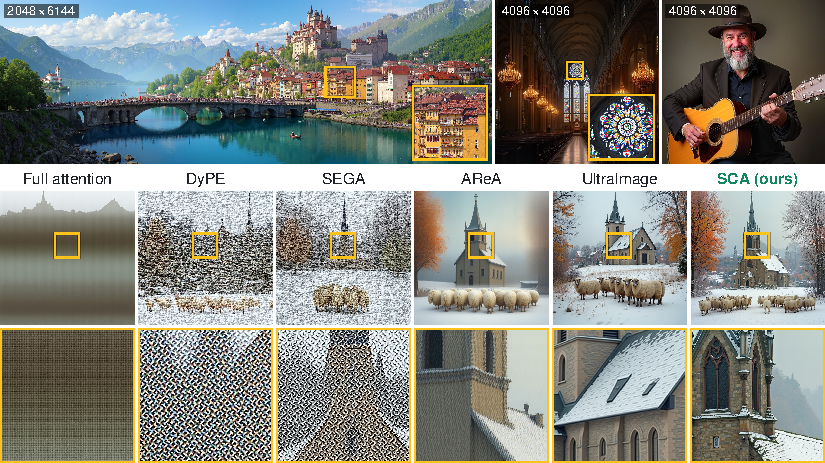
\includegraphics[width=\linewidth]{figures/teaser.pdf}
  \captionof{figure}{\textbf{\sca{} at 4K without training.} Top: curated \sca{} outputs of FLUX.1-dev at $2048\times6144$ and $4096^2$, with insets at native pixels. Bottom: one curated $4096^2$ prompt where no baseline scores unusually low, with 1:1 crops; full attention gives a flat field, DyPE and SEGA a lattice, and AReA, UltraImage, and \sca{} keep the church and flock.\pendImgTeaser}
  \label{fig:teaser}
\end{center}

% =====================================================================================
\section{Introduction}
\label{sec:intro}

Diffusion transformers~\citep{peebles2022dit} such as FLUX.1~\citep{flux2024} and Stable Diffusion~3~\citep{esser2024sd3} are trained near one megapixel. At $4096\times4096$ the image has 16 times as many tokens, full attention costs about 256 times as much, and every layer meets token counts and position offsets it never saw in training. FLUX.1-dev with full attention then returns stripes or a flat field (Figure~\ref{fig:teaser}, bottom left). Restricting each query to a native-size window keeps the offsets in range, yet run from the first step it draws five Moai where the prompt asks for one (Figure~\ref{fig:motivation}a). We ask whether each head's balance between such a window and a coarse view of the whole image can be measured at the training resolution, and when in sampling each head should receive its window.

\begin{wrapfigure}{r}{0.42\linewidth}
  \wraptop
  \centering
  \begin{minipage}[t]{0.495\linewidth}\centering
    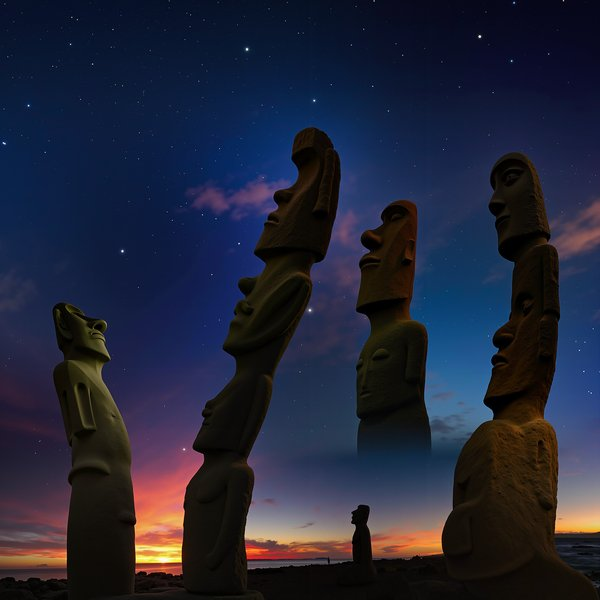
\includegraphics[width=\linewidth]{figures/failure/moai_v0w64.jpg}\\[1pt]
    {\sffamily\scriptsize (a) mix from step 1}
  \end{minipage}\hfill
  \begin{minipage}[t]{0.495\linewidth}\centering
    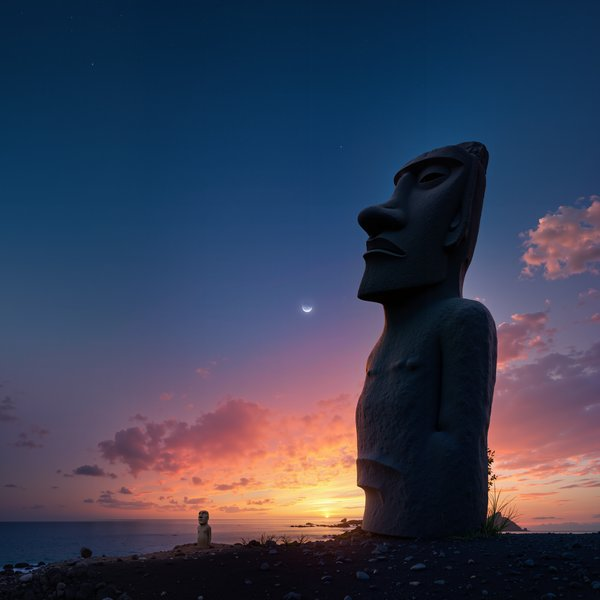
\includegraphics[width=\linewidth]{figures/failure/moai_sca.jpg}\\[1pt]
    {\sffamily\scriptsize (b) global opening}
  \end{minipage}
  \caption{\textbf{Windows repeat the subject.} A development prompt asking for one Moai at $4096^2$. (a)~Native-size windows mixed in from step 1 draw five; (b)~a global-only opening keeps one large statue, plus a small one far off.}
  \label{fig:motivation}
  \wrapbot
\end{wrapfigure}
Training-free fixes either edit the positional encoding~\citep{zhuo2024lumina,issachar2025dype,zhao2025ultraimage,rajabi2026sega} or restrict the keys each query sees~\citep{zhang2023hidiffusion,ma2025resdit,xue2026hrdit,rajabi2026area}. A native-size window cannot see an object larger than itself, so whenever windows dominate while a subject is still forming, each window may settle that subject alone. AReA~\citep{rajabi2026area}, the most recent key-restricting method, attends to pooled keys for the first 8 of 28 steps and then to windows that shrink to native size, with one schedule for all heads. HRDiT and UltraImage give heads their own receptive fields, by cost budget or entropy~\citep{xue2026hrdit,zhao2025ultraimage}. None measures a head's balance at the training resolution, where full attention is trustworthy (Section~\ref{sec:related}).

We answer by emulation. To mimic a target $s$ times larger, we shrink both a native-size neighbourhood and a downsampled view of the whole image by $s$, so the image-to-window ratio matches the target while full attention stays in distribution and serves as ground truth. A convex mix of the two views fits each head in closed form. Its weight differs strongly between heads, is stable across prompt splits (correlation 0.99), and transfers: the emulated scale-2 table explains scale 4 with 2.4\% more output error than the scale-4 table (Section~\ref{sec:analysis}). We call this measured transfer scale covariance; the weight depends mainly on the image-to-window ratio, so one table serves every window size.

We introduce Scale-Covariant Attention (\sca{}), which turns this measurement into an attention operator (Figure~\ref{fig:method}). Each head mixes a global branch over block-centre keys, placed at coarse positions inside the native grid, with a local branch, an exact sliding window. One schedule sets the window: the whole image, seen at native size by the global branch, for the first 8 of 28 steps, then windows of 128, 112, 96, and 80 tokens, then the native 64. At every step each head's weight is read from the calibration table at the current image-to-window ratio. The local softmax also holds 1,024 bridge tokens sampled across the image, so a window can see a subject drawn outside it.

The schedule comes from a failure we measured. Our first operator switched every head from the global view to a native window in one step, at a weight near 0.7 that calibration gives almost regardless of noise level. Each window then redrew small subjects: a detector finds a duplicated person or animal in 57\% of the 95 prompts that name one at $4096^2$, against 4\% for AReA (Section~\ref{sec:dup}). \hlDupIntro{} With the schedule, \sca{} beats AReA on \hlWinsArea{} of \hlMetricsArea{} metrics at $4096^2$, at \hlSecSca\,s per image against \hlSecArea\,s (Section~\ref{sec:main}). We highlight our contributions below.
\begin{itemize}
  \item We fit each head's mix of local and global attention in closed form at the training resolution, for every noise level and image-to-window ratio, and show that the fit transfers across scales (Section~\ref{sec:analysis}).
  \item We trace the repeated subjects of windowed attention to a one-step switch from the global view to native windows, and remove most of them with a schedule that shrinks each window and reads each head's weight at the matching ratio (Sections~\ref{sec:rootcause} and~\ref{sec:dup}).
  \item We show that at $4096^2$ on FLUX.1-dev, \sca{} beats AReA on \hlWinsArea{} of \hlMetricsArea{} metrics with paired 95\% intervals excluding zero, loses \hlLossesAreaWord{}, and runs $\hlSpeedArea\times$ faster.
\end{itemize}

\begin{figure}[t]
  \centering
  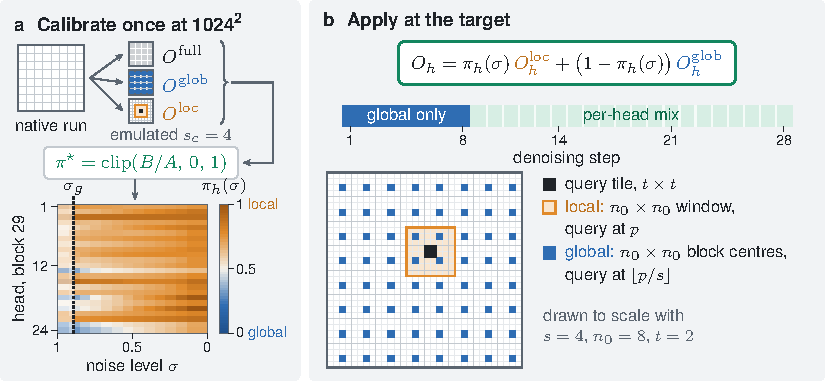
\includegraphics[width=\linewidth]{figures/method.pdf}
  \caption{\textbf{\sca{} sampling and calibration.} (a)~After the global-only opening, the window shrinks from 128 to 64 tokens and its softmax adds 1,024 bridge tokens (schematic dots); each head weighs the branches by $\pi_h$ read at $r=\max(H,W)/w$. (b)~At $1024^2$, $\pi$ per head and noise bin is fitted to full attention at emulated ratios 2 and 4; Figure~\ref{fig:method_zoom} zooms in.}
  \label{fig:method}
\end{figure}

% =====================================================================================
\section{Scale-Covariant Attention}
\label{sec:method}

\subsection{Setting and notation}
\label{sec:setting}
A multimodal diffusion transformer such as FLUX.1 concatenates $T$ text tokens $\Tset$ with $N=HW$ image tokens on the grid $\Gset=[H]\times[W]$, where $[n]=\{0,\dots,n-1\}$. Each block applies joint attention (57 blocks of 24 heads in FLUX.1). It is trained at about $1024^2$ pixels, a native grid of $n_0\times n_0$ tokens with $n_0=64$. Rotary embeddings~\citep{su2021roformer} give token $j$ a position $p_j\in\mathbb{Z}^2$ (FLUX.1 puts all text tokens at $0$) and a rotation $R_p$ with $R_p^\top R_{p'}=R_{p'-p}$. For one head, a pre-rotation query $q$ placed at $u$, and a set $\Kset$ of (key, value, key position) triples,
\begin{equation}
  \Attn(q,u;\Kset) \;=\; \textstyle\sum_{(k,v,u')\in\Kset} \operatorname{softmax}_{\Kset}\!\big(q^\top R_{u'-u}\,k/\sqrt d\big)\; v ,
  \label{eq:attn}
\end{equation}
where $d$ is the head dimension. Full attention is $\Ofull_i=\Attn\big(q_i,p_i;\{(k_j,v_j,p_j)\}_{j\in\Tset\cup\Gset}\big)$. The target grid is $H=s_H n_0$, $W=s_W n_0$ with integer factors ($s$ when equal), so full attention meets offsets $s$ times the trained range. The latent at noise level $\sigma$ is $x_\sigma=(1-\sigma)x_0+\sigma\epsilon$. Splitting the keys into a near and a far set gives exactly $\Ofull_i=m_iO^{\mathrm{near}}_i+(1-m_i)O^{\mathrm{far}}_i$ (Lemma~\ref{lem:split}), where each $O$ attends only to its own set and $m_i$ is the softmax mass on the near set. Every head is thus a query-dependent mix of a near and a far field, which \sca{} approximates with two separately normalized operators and one weight per head.

\subsection{Two operators}
\label{sec:branches}

\paragraph{Global operator.} Let $\Gnat=[H/s_H]\times[W/s_W]$ be the $n_0\times n_0$ grid of blocks. Block-centre subsampling keeps for each block $b$ the token at $\kappa(b)=(s_H b_1+\lfloor s_H/2\rfloor,\, s_W b_2+\lfloor s_W/2\rfloor)$. The coarse map $c(p)=(\lfloor p_1/s_H\rfloor,\lfloor p_2/s_W\rfloor)$ sends a position to its block, so $c(\kappa(b))=b$, and
\begin{equation}
  \Kset^{\mathrm{glob}}=\{(k_j,v_j,0)\}_{j\in\Tset}\cup\{(k_{\kappa(b)},v_{\kappa(b)},b)\}_{b\in\Gnat},\qquad
  \Oglob_i=\Attn\big(q_i,\,c(p_i);\,\Kset^{\mathrm{glob}}\big),
  \label{eq:glob}
\end{equation}
with $c(p_i)$ replaced by 0 for text queries. This is AReA's first phase with the pooling factor fixed at $s$: the whole image shown as one native canvas. It models content whose extent is a fixed fraction of the image: layout, object count, identity.

\paragraph{Local operator.} Image queries form tiles of $t\times t$ tokens ($t=8$); query $i$ lies in tile $\tau=\lfloor p_i/t\rfloor$. The window $\Win_w(i)$ of tile $\tau$ has side $w$ (at most the grid side) and starts at $a(\tau)=\mbox{$\clip\big(t\tau+\lfloor t/2\rfloor-\lfloor w/2\rfloor,0,H-w\big)$}$ per axis, centred on the tile and clamped to the grid. Its keys are the text tokens, a bridge set $\mathcal{B}$ of image tokens, and the window, all at their original positions:
\begin{equation}
  \Kset^{\mathrm{loc}}_i(w)=\{(k_j,v_j,0)\}_{j\in\Tset}\cup\{(k_j,v_j,p_j)\}_{j\in\mathcal{B}\cup\Win_w(i)},\qquad
  \Oloc_i(w)=\Attn\big(q_i,\,p_i;\,\Kset^{\mathrm{loc}}_i(w)\big).
  \label{eq:loc}
\end{equation}
The bridge takes, in each cell $c$ of an $8\times8$ partition of the grid, the 16 tokens whose pre-rotation keys lie farthest from the mean image key $\bar k^{h}$, summed over heads $h$:
\begin{equation}
  \mathcal{B}=\textstyle\bigcup_{c}\operatorname{top}_{16}\big\{\sum_{h}\|k^{h}_j-\bar k^{h}\|^2 : j\in c\big\},
  \label{eq:bridge}
\end{equation}
recomputed at every block and step. This is AReA's selection rule~\citep{rajabi2026area}. Keys form a multiset, so a bridge token inside the window enters twice. With $w=n_0$ the window is an exact native-size sliding window, which models content whose extent is fixed in tokens: edges, texture, fine structure. The 1,024 bridge tokens let a window see a subject drawn far outside it. Appendix~\ref{app:proofs} proves the two propositions below.

\begin{proposition}[Trained position range]
\label{prop:range}
Assume exact integer positions and $t\le n_0\le\min(H,W)$. Every query-key offset of the global operator, and every offset between an image query and a key of its window $\Win_{n_0}(i)$, is at most $n_0-1$ per axis. Each query of the global operator sees the native $T+n_0^2$ keys.
\end{proposition}

\begin{proposition}[Cost]
\label{prop:cost}
Per head and layer, full attention scores $(N+T)^2$ query-key pairs, the global operator $(N+T)(T+N_0)$ with $N_0=|\Gnat|=n_0^2$, and the local operator $N(T+R+w^2)$ with $R=|\mathcal{B}|$. For fixed $n_0$, $w$, $R$, and $T$ the total is $O\big(N(T+R+w^2+N_0)\big)$, linear in $N$.
\end{proposition}
The bridge keys keep their true positions, and windows wider than $n_0$ reach offsets up to $w-1$, so the local operator leaves the trained range for 1,024 of its keys and during the four wide-window steps. FLUX.1 also rounds positions in bf16 beyond 256 tokens per axis (Appendix~\ref{app:impl}).

\paragraph{Design choices.} A block centre is a real token, so the global branch attends to keys and values the model produced; mean pooling instead lowers ImageReward by 1.52 (Section~\ref{sec:ablations}). A native window of side $n_0$ keeps window offsets in the trained range, so \sca{} keeps FLUX.1's RoPE and softmax scale; text keys sit at position 0 in both branches (Remark~\ref{rem:text}).

\paragraph{Worked example.} At $4096^2$ the latent grid is $256\times256$ tokens ($s=4$, $N=65{,}536$, $T=512$). The global branch keeps one centre per $4\times4$ block, 4,096 keys on a $64\times64$ grid, so with the text a query sees 4,608 keys. In the native-window phase each $8\times8$ query tile attends to the $64\times64$ window around it, the 1,024 bridge tokens, and the text: \hlWorkedLocalKeys{} keys, against 66,048 keys at offsets up to 255 in full attention. Over the 28 steps \sca{} scores \hlWorkedPairsRatio{} times fewer query-key pairs than full attention (Table~\ref{tab:flops}).

\begin{figure}[t]
  \centering
  \begin{minipage}[t]{0.48\linewidth}
    \hrule height 0.6pt\vspace{2pt}
    \captionof{algorithm}{\textbf{Calibration}, once per model}
    \label{alg:calib}
    \vspace{-4pt}
\begin{lstlisting}[style=scacode, emph={calibrate,attn,global_branch,local_branch,clip,fill_empty_bins}]
# Input: prompts; full-attention sampler at (*@$1024^2$@*)
# Output: pi*[s_c, l, h, beta]; full in App. (*@\ref{app:code}@*)
def calibrate(q, k, v, l, sigma):  # every block
  O_full = attn(q, k, v)        # Eq. (*@\ref{eq:attn}@*), all keys
  beta = min(int(14 * sigma), 13)    # noise bin
  for s_c in (2, 4):            # r = n / w = s_c
    f, w = s_c, n // s_c        # subsample, window
    t_c = round(t * w / n0)     # tile t n/(s_c n0)
    O_glob = global_branch(q, k, v, f)    # Eq. (*@\ref{eq:glob}@*)
    O_loc = local_branch(q, k, v, w, t_c) # Eq. (*@\ref{eq:loc}@*)
    dl, df = O_loc - O_glob, O_full - O_glob
    A[s_c, l, :, beta] += sum(dl * dl)    # Eq. (*@\ref{eq:stats}@*)
    B[s_c, l, :, beta] += sum(df * dl)  # over rows
    E[s_c, l, :, beta] += sum(df * df)
  return O_full                 # sampler unchanged
pi = clip(B / A, 0, 1); pi[A == 0] = 1  # Prop. (*@\ref{prop:opt}@*)
pi = fill_empty_bins(pi)  # read at r, Eq. (*@\ref{eq:sched}@*)
\end{lstlisting}
  \end{minipage}\hfill
  \begin{minipage}[t]{0.48\linewidth}
    \hrule height 0.6pt\vspace{2pt}
    \captionof{algorithm}{\textbf{Sampling}, one \sca{} attention call}
    \label{alg:sample}
    \vspace{-4pt}
\begin{lstlisting}[style=scacode, emph={rope,sdpa,cat,window,bridge,flex_layout,flex_attention,interp}]
# Input: q, k, v (T text, then H x W image), l, (*@$\sigma$@*)
# Output: O for all T + HW queries; App. (*@\ref{app:code}@*)
fh, fw = H // n0, W // n0       # subsampling s
kb = k_img[fh//2::fh, fw//2::fw]  # (*@$\kappa(b)$@*); vb alike
Q = cat(rope(q_txt, 0), rope(q_img, c(p)))
K = cat(rope(k_txt, 0), rope(kb, b))
O_glob = sdpa(Q, K, cat(v_txt, vb))     # Eq. (*@\ref{eq:glob}@*)
if sigma > sigma_g:                 # 0.89, Eq. (*@\ref{eq:mix}@*)
  return O_glob       # opening phase: no local
w = window(sigma)   # 128, 112, 96, 80, n0; Eq. (*@\ref{eq:sched}@*)
B = bridge(k_img, cells=8, k=16)  # Eq. (*@\ref{eq:bridge}@*), 1,024
Kl = cat(k_txt, k_img[B], k_img)  # Vl alike
mask = flex_layout(T + len(B), t=8, w=min(w, H))
O_loc = flex_attention(rope(q_img, p),  # Eq. (*@\ref{eq:loc}@*)
    rope(Kl, p_Kl), Vl, block_mask=mask)  # App. (*@\ref{app:impl}@*)
pi = interp(sigma, max(H,W)/w, table[l])  # ratio r
O_img = pi*O_loc + (1-pi)*O_glob[T:]    # Eq. (*@\ref{eq:mix}@*)
return cat(O_glob[:T], O_img)     # text: O_glob
\end{lstlisting}
  \end{minipage}
\end{figure}

\subsection{One schedule from the global view to the native window}
\label{sec:sched}
Calibration (Section~\ref{sec:calib}) gives each head $h$ of block $l$ a weight $\pi_{lh}(\sigma;r)$ for every noise level and every image-to-window ratio $r$ it emulates, here $r\in\{2,4\}$. At the target, a window schedule $w(\sigma)$ sets the ratio $r(\sigma)=\max(H,W)/w(\sigma)$, and an image query takes
\begin{equation}
  O_i \;=\; \begin{cases} \Oglob_i & \sigma>\sigma_g,\\ \pi\,\Oloc_i\big(w(\sigma)\big) + (1-\pi)\,\Oglob_i & \text{otherwise,}\end{cases}\qquad \pi=\pi_{lh}\big(\sigma;r(\sigma)\big),
  \label{eq:mix}
\end{equation}
where $\sigma_g$ is the gate, text queries take $\Oglob_i$, and the weight between calibrated ratios is interpolated linearly in $\log r$,
\begin{equation}
  \pi_{lh}(\sigma;r)=(1-\lambda)\,\pi_{lh}(\sigma;2)+\lambda\,\pi_{lh}(\sigma;4),\qquad \lambda=\clip(\log_2 r-1,\,0,\,1).
  \label{eq:sched}
\end{equation}
We use $\sigma_g=0.89$, the first 8 of 28 steps at maximum shift as in AReA, and $w=128$, 112, 96, and 80 tokens for $\sigma$ in $(0.88,0.89]$, $(0.86,0.88]$, $(0.84,0.86]$, and $(0.82,0.84]$, then $w=n_0$. At $4096^2$ these are the four steps after the opening, at ratios 2, 2.29, 2.67, and 3.2, and the last 16 steps run at ratio 4. The opening is the end of the schedule where the window is the whole image, which only the global branch can show at native size. Setting $w=n_0$ on every step after the gate gives a one-step switch, the operator we call \sca{} without the schedule. The schedule's four sizes were set by hand; only the weights are calibrated.

\subsection{Why a one-step switch repeats small subjects}
\label{sec:rootcause}
Without the schedule, small copies of the subject form in the steps right after the gate (Figure~\ref{fig:dup}c). Three measurements locate the cause. \textbf{The calibrated weights are flat in the noise level.} At scale 4 the mean $\pih$ over the 1368 heads is 0.69 at $\sigma=0.90$ and 0.77 at $\sigma=0.11$, and 80\% of heads exceed 0.5 at the gate, so the local branch jumps from weight 0 to about 0.7 in one step. \textbf{A native window is a native canvas.} A $64\times64$ window with native offsets and all 512 text keys matches the model's $1024^2$ training input, and we hypothesize that the trained prior fills such a canvas with the prompt's subject while objects of 6 to 25 tokens are still forming. \textbf{Duplication falls as the global view lasts longer.} On a fixed 46-prompt subset, people or animals repeat in 20, 15, and 7 of the 26 prompts that name them for gates at $\sigma=0.93$, 0.89, and 0.85, and in 1 of 26 with the global branch alone (Figure~\ref{fig:dup}a). A later gate is no cure: gate 0.85 lowers the aesthetic score by 0.19 and MUSIQ$_\text{c}$ by 2.0. Progressive \sca{}, whose $1024^2$ stage fixes the layout before any window opens, repeats subjects in 8\% of prompts.

The schedule hands over in four steps instead of one, through windows that each hold more than a native canvas, and the bridge shows every window what is drawn elsewhere. Reading the weight at the matching ratio matters for quality: with the scale-4 weight on 128-token windows, prompts that never had duplicates lose ImageReward, HPSv2, ARNIQA, and MUSIQ$_\text{c}$, and matched weights remove most of that loss (Appendix~\ref{app:dupfix}). Argument~\ref{arg:freq} in Appendix~\ref{app:proofs} gives a frequency view of why windows fail at high noise.

\subsection{Calibration by output matching}
\label{sec:calib}
The weights must come from where the model is trustworthy, which the target is not. On an in-distribution $n\times n$ grid ($n=64$ at $1024^2$), emulated ratio $r$ uses subsampling factor $r$, window side $n/r$, and tile side $\mathrm{round}(tn/(rn_0))$, so the ratio of grid to window is $r$, as at a target of scale $r$. The sampler runs unmodified full attention (Algorithm~\ref{alg:calib}), and at every block and step both emulated operators see the same queries, keys, and values. For block $l$, head $h$, noise bin $\beta$, and ratio $r$, sums over prompts, steps with $\sigma\in\beta$, image queries, and channels give
\begin{equation}
  A=\textstyle\sum\|\Oloc-\Oglob\|^2,\quad
  B=\sum\langle \Ofull-\Oglob,\,\Oloc-\Oglob\rangle,\quad
  E=\sum\|\Ofull-\Oglob\|^2,
  \label{eq:stats}
\end{equation}
where $\Oloc,\Oglob$ are emulated without the bridge. The mix with weight $\pi$ has squared error $J(\pi)=E-2\pi B+\pi^2A$.

\begin{proposition}[Closed-form calibration and transfer cost]
\label{prop:opt}
In each cell $(l,h,\beta,r)$, $J$ is minimized on $[0,1]$ by $\pi^\star=\clip(B/A,0,1)$, with $\pi^\star=1$ if $A=0$. Any other weight $\pi'\in[0,1]$ (fitted at another ratio or resolution, per layer, shared, or a hard switch) has $J(\pi')-J(\pi^\star)\ge A(\pi'-\pi^\star)^2$, with equality when $0<\pi^\star<1$.
\end{proposition}
So the per-head table has the lowest output error of any rule constant within a cell, and replacing it costs an $A$-weighted squared distance. The same sums score every alternative rule without another forward pass, and one pass collects ratios 2 and 4. At inference each step interpolates a head's weight linearly in $\sigma$ between the mean noise levels of occupied bins (14 of width $1/14$), constant beyond them, and in $\log r$ by Eq.~\ref{eq:sched}; the native-window phase reads the ratio nearest $\max(s_H,s_W)$ in log space, here always 4. The local operator is one exact FlexAttention call with the text and bridge keys as a shared prefix~\citep[Algorithm~\ref{alg:sample}]{dong2024flex}.

\subsection{\texorpdfstring{\sca{}}{SCA} inside a progressive schedule}
\label{sec:progressive}
\sca{} replaces only the attention, so it fits inside a multi-stage sampler (Algorithm~\ref{alg:prog}). HRDiT's released code~\citep{xue2026hrdit} denoises at $1024^2$ for 30 steps, then upsamples, re-noises, and repeats the last 17 and 10 steps of the same schedule at $2048^2$ and $4096^2$, with NTK-scaled RoPE, a proportional attention scale, per-head key pruning, and position alignment. Progressive \sca{} keeps HRDiT's schedule, transitions, guidance, and seeds and replaces those four attention changes with \sca{}. Its stages re-enter at $\sigma=0.81$ and $0.61$, below the last wide window, so the $1024^2$ stage sets the layout and only the native window and the bridge run.

\begin{figure}[t]
  \centering
  \IfFileExists{figures/dup.pdf}{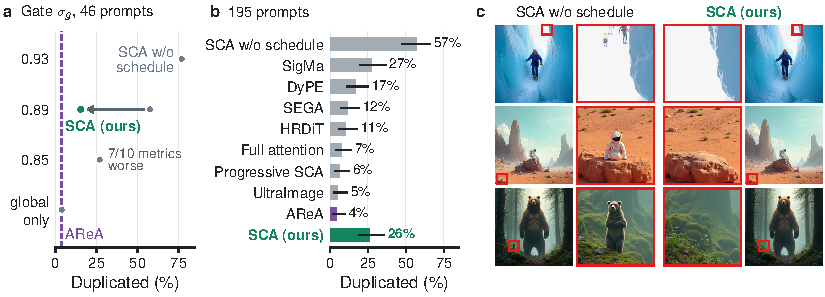
\includegraphics[width=\linewidth]{figures/dup.pdf}}{\fbox{\parbox[c][1.6in][c]{0.95\linewidth}{\centering duplication figure}}}
  \caption{\textbf{A gradual handover cuts late duplication.} (a)~Duplicated person or animal prompts of the 46-prompt subset against the gate; a later gate costs quality, so ours keeps $\sigma_g=0.89$ and adds the schedule. (b)~All methods, 95 such prompts at $4096^2$. (c)~Uncurated, same seed, chosen as in Appendix~\ref{app:dupfix}; one astronaut copy remains.}
  \label{fig:dup}
\end{figure}

% =====================================================================================
\section{What the heads want}
\label{sec:analysis}

\begin{figure}[t]
  \centering
  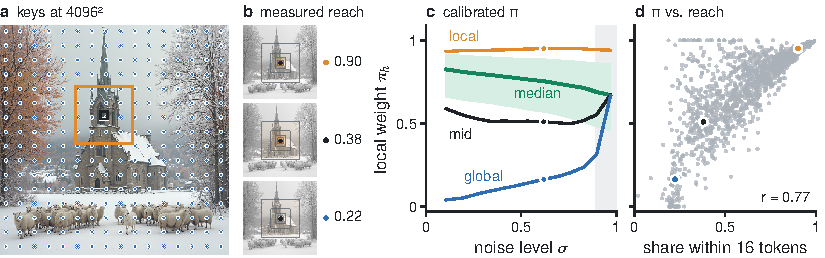
\includegraphics[width=\linewidth]{figures/heads_view.pdf}
  \caption{\textbf{Measured reach tracks calibrated $\pi_h$.} (a)~Query tile, local window (amber), and every fourth block-centre key per axis (blue) on a $4096^2$ \sca{} output; (b)~full-attention mass of three heads at $1024^2$, averaged over the 32 calibration prompts. (c)~Their scale-2 $\pih$ with the median and interquartile range of all 1368 heads (grey: global only); (d)~$\pi_h$ against the mass share within 16 tokens, printed in (b), at $\sigma=0.62$ ($r=0.77$).}
  \label{fig:heads}
\end{figure}
We calibrate FLUX.1-dev on 32 purpose-written prompts at $1024^2$ and 16 at $1280^2$, disjoint from the evaluation sets. Errors are relative, $\sum J/\sum\|\Ofull\|^2$, pooled over blocks, heads, and steps.

\paragraph{Heads differ, and each head's weight depends on the ratio.} In the scale-2 table the standard deviation of $\pih$ over the 1368 heads is 0.24 to 0.26 at every noise level, and half of the (head, noise level) cells lie in $[0.2,0.8]$ (Figures~\ref{fig:heads}c, \ref{fig:pi_heads}, and~\ref{fig:calib}). At $\sigma=0.62$ a head's scale-2 weight tracks its share of full-attention mass within 16 tokens of the query ($r=0.77$; Figure~\ref{fig:heads}d). The mean weight is lower at ratio 2 than at ratio 4 at every noise level (0.65 against 0.69 at $\sigma=0.90$), so a wider window takes less local weight.

\paragraph{The table is stable and transfers.} Tables fitted on disjoint prompt halves correlate at 0.989 over all cells (0.986 at scale 4). Applied at scale 4, the scale-2 table gives 0.205 against 0.200 for the scale-4 table, below every shared rule fitted at scale 4; the $1024^2$ table scored at $1280^2$ gives 0.0589 against 0.0585. As the two resolutions emulate scale 2 with windows of 32 and 40 tokens, the weights appear to depend mainly on the image-to-window ratio, which is what Eq.~\ref{eq:sched} assumes.

\paragraph{Per-head beats coarser rules; output error misses layout.} Against the best hard switch, per-head mixing lowers the relative error from 0.092 to 0.057 at scale 2 and from 0.261 to 0.200 at scale 4; per-layer tables reach 0.071 and 0.223, and one shared weight per noise level 0.077 and 0.230 (Figure~\ref{fig:relerr}). A tokenwise squared error cannot see repeated subjects, so the opening and the schedule deliberately override the fit at high noise (Section~\ref{sec:rootcause}).

% =====================================================================================
\section{Experiments}
\label{sec:experiments}

\begin{table}[t]
  \caption{\textbf{Main comparison at $4096^2$.} FLUX.1-dev, \nmain{} Aesthetic-4K prompts, seed label 0; HPSv2.1 $\times100$, MUSIQ$_\text{c}$ on $1024^2$ crops, FID$_\text{p}$ patch FID, Dup.\ share of the 95 person or animal prompts with a duplicate; \textbf{best}, \underline{second best}, ours shaded; seconds per image on one GH200 as a clean batch-1 median or a campaign mean on shared nodes (camp.), n/m not measured; Table~\ref{tab:all_metrics} adds all metrics.\pendTabMain{} Key result: among single-pass methods, \sca{} is best on every quality metric shown and $\hlSpeedArea\times$ faster than AReA.}
  \label{tab:main}
  \centering\footnotesize
  % Generated by paper/figures/src/gen_main_tables.py from results/; do not edit by hand.
\setlength{\tabcolsep}{3.1pt}
\begin{tabular}{@{}lcrr*{7}{r<{\hspace{3pt}}}@{}}
  \toprule
   & & \multicolumn{2}{c}{Time (s)$\downarrow$} & Image$\uparrow$ & $\uparrow$ & Pick$\uparrow$ & $\uparrow$ & $\uparrow$ & $\downarrow$ & $\downarrow$ \\
  \cmidrule(lr){3-4}
  Method & Steps & clean & camp. & Reward & HPSv2.1 & Score & CLIP & MUSIQ$_\text{c}$ & FID & FID$_\text{p}$ \\
  \midrule
  \multicolumn{11}{@{}l}{\emph{Single pass, shared sampler (28 steps, guidance 4.5)}} \\
  Full attention & 28 & 186.5 & 196.2 & $-2.18$ & 7.60 & 17.94 & 15.37 & 33.1 & 312.4 & 252.2 \\
  DyPE & 28 & n/m & 195.9 & $-0.10$ & 20.55 & 20.51 & 24.92 & 50.3 & 205.5 & 171.9 \\
  SEGA & 28 & n/m & 190.4 & 0.56 & 24.34 & 21.64 & 26.95 & 50.3 & 164.9 & 125.8 \\
  AReA & 28 & 202.4 & 264.4 & 0.92 & 27.16 & 22.36 & 27.69 & 50.4 & 145.8 & \underline{102.9} \\
  \rowcolor[HTML]{EAF4F1}\textbf{\sca{} (ours)} & 28 & \textbf{71.1} & \textbf{71.5} & 1.23 & 29.67 & 23.09 & \textbf{29.14} & \textbf{61.2} & \textbf{138.1} & \textbf{99.1} \\
  \midrule
  \multicolumn{11}{@{}l}{\emph{Multi-stage, own recipe and budget}} \\
  UltraImage & 30+30 & n/m & 308.5 & \underline{1.28} & \underline{30.77} & \underline{23.33} & 28.84 & 41.7 & 142.0 & 109.5 \\
  HRDiT & 30+17+10 & \underline{108.6} & \underline{110.4} & \textbf{1.34} & \textbf{30.92} & \textbf{23.46} & \underline{29.12} & \underline{53.5} & \underline{138.4} & 103.0 \\
  \bottomrule
\end{tabular}%

\end{table}

\paragraph{Data and seeds.} The main set is the Aesthetic-4K evaluation split with 4K references~\citep{zhang2025diffusion4k}: \ifmainfull{all 195 prompts; four of them (\devprompts) were used during development, which favours \sca{} slightly}{\nmain{} prompts after excluding the four used during development (\devprompts)}. A fixed \nabl-prompt subset, chosen before any ablation ran, serves the ablations and the choice of the schedule, which therefore saw 46 of the 195 evaluation prompts. We also evaluate \ifhrgenfull{all 1000}{the first \nhrgen{} of the 1000} HRGen-1K prompts~\citep{rajabi2026area}, which have no references. Sizes are $4096^2$, $2048\times4096$, and $2048\times6144$ (height$\times$width), plus $6144^2$ and $8192^2$ for the operator without the schedule. Seeds hash the prompt id and seed label 0 and are shared by all methods; labels 1 and 2 repeat \ifseedfull{all prompts}{\nseed{} prompts}.

\paragraph{Models and baselines.} The main model is FLUX.1-dev~\citep{flux2024}; FLUX.1-Krea-dev (\nkrea{} prompts, against AReA) and FLUX.2-dev (50 prompts, against full attention, without the schedule), each calibrated on 16 prompts at $1024^2$, test other checkpoints. \sca{} uses $t=8$, $n_0=64$, $\sigma_g=0.89$, the window schedule of Section~\ref{sec:sched}, and the calibrated table at every size (Table~\ref{tab:hparams}). Full attention, AReA from its released code (Appendix~\ref{app:area}), DyPE~\citep{issachar2025dype}, SEGA~\citep{rajabi2026sega}, and SigMa~\citep{zhao2026sigma} share AReA's sampler: 28 Euler flow-matching steps, guidance 4.5, shift $\mu=1.15$, bf16, and tiled VAE decoding. UltraImage~\citep{zhao2025ultraimage} runs its guided two-stage recipe (30 steps per stage) and HRDiT~\citep{xue2026hrdit} its progressive recipe, each with its own budget (Appendix~\ref{app:additional_protocols}). Each process uses one NVIDIA GH200 120GB; worker logs give at least 123.3 GH200-hours for the operator without the schedule (Appendix~\ref{app:compute}).

\begin{figure}[t]
  \centering
  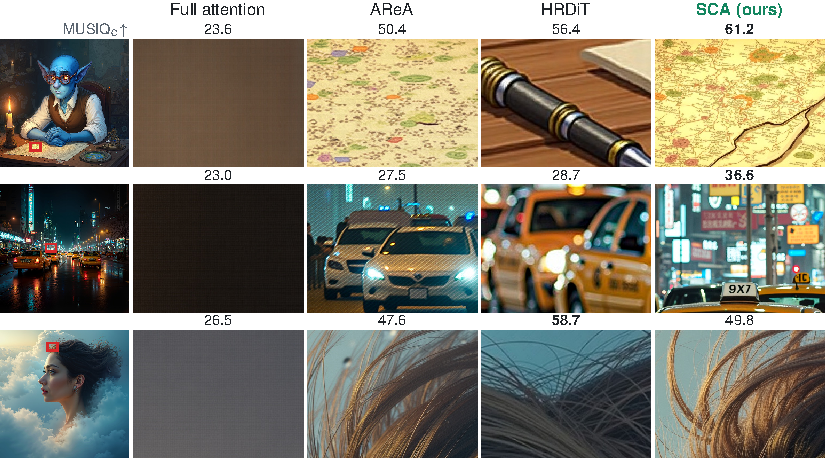
\includegraphics[width=\linewidth]{figures/zoom4k.pdf}
  \caption{\textbf{\sca{} keeps native detail at $4096^2$.} Three curated prompts (seed~0; curation favours \sca{}): \sca{}'s image, then each method's red window at 1:1 under its MUSIQ$_\text{c}$ (best bold). Full attention collapses to flat texture; Table~\ref{tab:main} gives means and Figure~\ref{fig:gallery_4096} uncurated samples.\pendImgQual}
  \label{fig:qual_main}
\end{figure}

\begin{wrapfigure}[21]{r}{0.46\linewidth}
  \wraptop
  \centering
  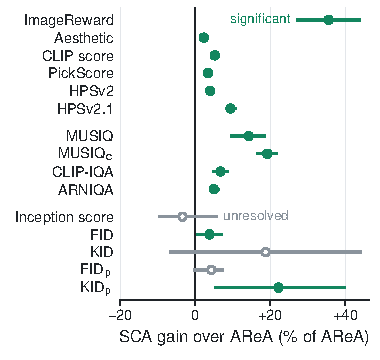
\includegraphics{figures/paired_area.pdf}
  \caption{\textbf{\hlWinsAreaWord{} of \hlMetricsArea{} metrics improve.} \sca{} minus AReA at $4096^2$ as percent of AReA's mean, with 95\% paired intervals. FID, KID, and their patch versions are negated so right is better; grey intervals span zero.\pendFigPaired}
  \label{fig:paired_area}
  \wrapbot
\end{wrapfigure}
\paragraph{Metrics.} Preference and alignment scores are ImageReward, HPSv2, HPSv2.1, PickScore, CLIP score, and aesthetic score~\citep{xu2023imagereward,wu2023hpsv2,kirstain2023pickapic,radford2021clip,schuhmann2022aesthetic}. No-reference quality is MUSIQ on the full image and over four $1024^2$ crops (MUSIQ$_\text{c}$), CLIP-IQA, and ARNIQA~\citep{ke2021musiq,wang2022clipiqa,agnolucci2024arniqa}. Distribution scores are FID and KID against all 195 official Aesthetic-4K references and Inception score at $299^2$, and patch FID and KID on the same crops~\citep{heusel2017fid,salimans2016improved}; patch FID is our own definition, so we never compare it across papers. Intervals are 95\% paired percentile bootstraps over prompt ids (1000 or 2000 draws), which also resample references for FID and KID (Appendix~\ref{app:metrics}).

\paragraph{Duplication.} An open-vocabulary detector, Grounding DINO~\citep{liu2023groundingdino}, counts every subject the prompt names in each image. An image is duplicated when a person or animal count exceeds the count the prompt implies; 95 of the 195 prompts imply one, and subject lists were written from the prompt text alone. On the 20 labelled images with people or animals, the detector agrees with our visual review on all 20 (Appendix~\ref{app:dupfix}).

\subsection{Main results}
\label{sec:main}

\paragraph{\sca{} beats AReA on \hlWinsAreaWord{} of \hlMetricsArea{} metrics at \textbf{$\hlSpeedArea\times$} the speed.} The gains include ImageReward (0.92 to \hlIrScaAbs, $\hlIrDelta$ $[\hlIrLo,\hlIrHi]$) and FID (145.8 to \hlFidScaAbs, $\hlFidDelta$ $[\hlFidLo,\hlFidHi]$); \hlUnresolvedAreaWord{} are unresolved (Tables~\ref{tab:main} and~\ref{tab:app_4k}; Figures~\ref{fig:teaser}, \ref{fig:qual_main}, and~\ref{fig:paired_area}). Our AReA run reproduces AReA's published FLUX.1-Krea-dev scores within 0.3 (Table~\ref{tab:published_compare}).

\paragraph{Every shared-sampler baseline trails \sca{} on all ten per-image metrics.} This holds for DyPE, SEGA, and SigMa (Tables~\ref{tab:phase2_baselines} and~\ref{tab:panel46_deltas}). UltraImage, at over four times \sca{}'s time, is significantly better on HPSv2.1 and PickScore and worse on CLIP score and both MUSIQ scores (Tables~\ref{tab:phase2_baselines} and~\ref{tab:phase2_distribution}). HRDiT's three-stage recipe leads single-pass \sca{} on learned preference scores at $\hlHrditTimeX\times$ its time (Table~\ref{tab:main}).

\begin{table}[t]
  \caption{\textbf{Multi-stage recipes and sampling budgets.} $4096^2$, \npanel{} prompts, campaign times, columns as in Table~\ref{tab:main} with the best in bold; against \sca{}, $^{+}$ is significantly better, $^{\circ}$ unresolved, and no mark significantly worse. Budget rows use the operator without the schedule.\pendTabPanel{} Key result: progressive \sca{} (HRDiT's schedule, \sca{} attention) matches HRDiT's preference scores at \hlCampProg\,s against \hlCampHrdit\,s; Tables~\ref{tab:panel46_deltas}, \ref{tab:phase2_budget}, and~\ref{tab:prog_deltas} add intervals.}
  \label{tab:panel46}
  \centering\footnotesize
  % Generated by paper/figures/src/gen_main_tables.py from results/; do not edit by hand.
\setlength{\tabcolsep}{2.4pt}
\begin{tabular}{@{}lcrr*{7}{r<{\hspace{2.5pt}}}r@{}}
  \toprule
   & & \multicolumn{2}{c}{Time (s)$\downarrow$} & Image$\uparrow$ & $\uparrow$ & Pick$\uparrow$ & $\uparrow$ & $\uparrow$ & $\downarrow$ & $\downarrow$ & $\downarrow$ \\
  \cmidrule(lr){3-4}
  Method & Steps & clean & camp. & Reward & HPSv2.1 & Score & CLIP & MUSIQ$_\text{c}$ & FID & FID$_\text{p}$ & Dup. \\
  \midrule
  \multicolumn{12}{@{}l}{\emph{Single pass, shared sampler (28 steps, guidance 4.5; other rows in Table~\ref{tab:main})}} \\
  SigMa & 28 & n/m & 192.5 & $-0.52$ & 18.65 & 20.01 & 23.51 & 49.9 & 216.9 & 184.6 & 27 \\
  \rowcolor[HTML]{EAF4F1}\textbf{\sca{} (ours)} & 28 & \pend{\textbf{71.1}} & \pend{71.5} & \pend{1.23} & \pend{29.67} & \pend{23.09} & \pend{29.14} & \pend{61.2} & \pend{\textbf{138.1}} & \pend{99.1} & \pend{57} \\
  \midrule
  \multicolumn{12}{@{}l}{\emph{Multi-stage, own recipe and budget}} \\
  UltraImage & 30+30 & n/m & 308.5 & 1.28\pend{\rlap{$^{\circ}$}} & 30.77\pend{\rlap{$^{+}$}} & 23.33\pend{\rlap{$^{+}$}} & 28.84 & 41.7 & 142.0 & 109.5 & \textbf{5} \\
  HRDiT & 30+17+10 & 108.6 & 110.4 & \textbf{1.34}\pend{\rlap{$^{+}$}} & 30.92\pend{\rlap{$^{+}$}} & \textbf{23.46}\pend{\rlap{$^{+}$}} & 29.12\pend{\rlap{$^{\circ}$}} & 53.5 & 138.4\pend{\rlap{$^{\circ}$}} & 103.0 & 11 \\
  \rowcolor[HTML]{EAF4F1}\textbf{Prog.\ \sca{}} & 30+17+10 & n/m & \pend{\textbf{49.5}} & \pend{1.32\rlap{$^{+}$}} & \pend{\textbf{30.99}\rlap{$^{+}$}} & \pend{23.42\rlap{$^{+}$}} & \pend{\textbf{29.36}\rlap{$^{\circ}$}} & \pend{54.2} & \pend{141.1\rlap{$^{\circ}$}} & \pend{106.3} & \pend{8} \\
  \midrule
  \multicolumn{12}{@{}l}{\emph{Without the schedule, other budgets}} \\
  \quad 56 steps & 56 & n/m & 139.9 & 1.26\rlap{$^{+}$} & 30.55\rlap{$^{+}$} & 23.22\rlap{$^{+}$} & 29.14\rlap{$^{\circ}$} & \textbf{64.1}\rlap{$^{+}$} & 139.8\rlap{$^{\circ}$} & 102.9 & 55 \\
  \quad guidance 7 & 28 & n/m & 71.9 & 1.16 & 29.07 & 22.82 & 28.94\rlap{$^{\circ}$} & 61.4\rlap{$^{\circ}$} & 140.4\rlap{$^{\circ}$} & \textbf{98.4}\rlap{$^{\circ}$} & 49 \\
  \quad 42 steps & 42 & n/m & 106.8 & 1.26\rlap{$^{\circ}$} & 30.27\rlap{$^{+}$} & 23.17\rlap{$^{+}$} & 29.14\rlap{$^{\circ}$} & 63.1\rlap{$^{+}$} & 140.5 & 100.6\rlap{$^{\circ}$} & 57 \\
  \bottomrule
\end{tabular}%

\end{table}

\paragraph{Progressive \sca{} matches HRDiT's preference scores in less than half the time.} HRDiT's lead thus comes from its schedule. Progressive \sca{} takes \hlCampProg\,s per image and HRDiT \hlCampHrdit\,s, as campaign means (Table~\ref{tab:panel46}; Figure~\ref{fig:progressive}). ImageReward differs by $\hlProgHrditIr$ $[\hlProgHrditIrLo,\hlProgHrditIrHi]$, HPSv2.1 by $\hlProgHrditHps$ $[\hlProgHrditHpsLo,\hlProgHrditHpsHi]$, and PickScore by $\hlProgHrditPick$ $[\hlProgHrditPickLo,\hlProgHrditPickHi]$, and no per-image metric is significantly worse; this does not establish equivalence (Table~\ref{tab:prog_deltas}). Against single-pass \sca{}, the parity costs fidelity, with higher patch FID and lower MUSIQ$_\text{c}$ (Appendix~\ref{app:budget}).

\subsection{Late duplication}
\label{sec:dup}

\paragraph{Without the schedule, \sca{} repeats people or animals more often than any baseline.} It does so in 57\% of the 95 prompts that name them, against 4\% for AReA, 7\% for full attention, and 27\% for SigMa (Figure~\ref{fig:dup}b). The rate stays at 50 to 57\% across three seeds, 42 or 56 steps, and guidance 7, and the operator without the schedule also repeats subjects at $2048\times4096$ (43\% against 18\% for AReA) and $2048\times6144$ (54\% against 6\%). \textbf{The schedule removes most of it.} \hlDupResults{} The copies it leaves are smaller and fewer, and Figure~\ref{fig:dup}c shows uncurated pairs, including one the schedule does not fix.

\subsection{Other sizes and latency}
\label{sec:sizes}

\begin{wrapfigure}[15]{l}{0.47\linewidth}
  \wraptop
  \centering
  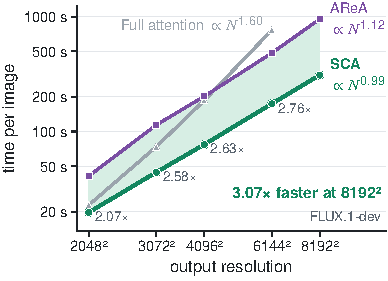
\includegraphics[width=\linewidth]{figures/latency_wrap.pdf}
  \caption{\textbf{Latency against size.} Batch 1, one GH200, median of three prompts; grey: speedup over AReA.\pendFigLatency}
  \label{fig:latency}
  \wrapbot
\end{wrapfigure}
\paragraph{\sca{} is the fastest method we timed at every size; quality depends on the aspect ratio.} At $2048\times6144$ \sca{} beats AReA on \hlWideSixWins{} metrics, and results are mixed at $2048\times4096$ (Table~\ref{tab:app_wide}). Without the schedule it also beats AReA on 14 of 15 metrics at $6144^2$ (ImageReward $+1.262$ $[1.051,1.450]$), and 12 exploratory prompts at $8192^2$ favour it on preference and alignment scores, though grid artifacts remain (Appendix~\ref{app:8k}).

\paragraph{\sca{}'s time grows nearly linearly with pixel count.} Fitting clean seconds $\propto N^b$ over the $N$ image tokens gives $b=\hlLatExpSca$ for \sca{} and 1.12 for AReA (Table~\ref{tab:latency}; Figure~\ref{fig:latency}, five sizes from $2048^2$ to $8192^2$). Clean time is the median of three images after warm-up on an idle GPU, including text encoding and VAE decoding but not model loading. The schedule and the bridge add \hlTimeOverhead\ to the time per image at $4096^2$. At $8192^2$ \sca{} takes \hlLatEightSca\,s against AReA's 952.0\,s, $\hlLatEightRatio\times$ faster.

\subsection{Ablations}
\label{sec:ablations}

\begin{table}[t]
  \centering
  \begin{minipage}[t]{0.47\linewidth}
    \caption{\textbf{Ablations.} $4096^2$, fixed \nabl-prompt subset; the shaded default row gives absolute values, the schedule rows the paired change against it, and the base-operator rows the change against \sca{} without the schedule; \textcolor{sigdn}{orange}: significantly worse, \textcolor{sigup}{blue}: better; IR, HPS, Pick, M$_\text{c}$: ImageReward, HPSv2.1 $\times100$, PickScore, MUSIQ$_\text{c}$; Dup.: duplicated person or animal prompts of 26; Err.: relative output error at scale 4; Table~\ref{tab:app_abl} adds all metrics.\pendTabAbl{} Key result: the schedule cuts duplication; every base-operator change lowers HPSv2.1 and PickScore.}
    \label{tab:ablation}
    \centering\footnotesize
    % Generated by paper/figures/src/gen_main_tables.py from results/; do not edit by hand.
\setlength{\tabcolsep}{1.4pt}
\begin{tabular}{@{}lrrrrr@{}}
  \toprule
  Variant & Err. & IR & HPS & Pick & M$_\text{c}$ \\
  \midrule
  \rowcolor[HTML]{EAF4F1}\sca{} (default) & 0.200 & 1.12 & 29.98 & 22.96 & 62.5 \\
  \midrule
  \multicolumn{6}{@{}l}{\emph{Weight rule after the opening phase}} \\
  local only & 0.261 & \dn{$-0.36$} & \dn{$-2.86$} & \dn{$-1.20$} & $-0.3$ \\
  shared $\pi(\sigma)$ & 0.230 & \dn{$-0.09$} & \dn{$-1.83$} & \dn{$-0.38$} & \dn{$-10.4$} \\
  per-layer $\pi_\ell(\sigma)$ & 0.223 & $-0.05$ & \dn{$-0.70$} & \dn{$-0.16$} & \dn{$-2.4$} \\
  \multicolumn{6}{@{}l}{\emph{Global branch and opening phase}} \\
  global only & 0.627 & \dn{$-0.40$} & \dn{$-5.66$} & \dn{$-1.44$} & \dn{$-11.7$} \\
  mean pooling & n/a & \dn{$-1.52$} & \dn{$-9.75$} & \dn{$-2.60$} & \dn{$-4.2$} \\
  no opening (v0) & 0.200 & \dn{$-1.33$} & \dn{$-4.07$} & \dn{$-2.18$} & $+2.5$ \\
  \bottomrule
\end{tabular}%

  \end{minipage}\hfill
  \begin{minipage}[t]{0.47\linewidth}
    \caption{\textbf{Generality and sensitivity.} Paired differences at $4096^2$ against each group's reference; $n$: prompts; \textcolor{sigdn}{orange} if significantly worse; sensitivity rows vary the operator without the schedule (32 calibration prompts, $\sigma_g=0.89$); Tables~\ref{tab:phase2_general}, \ref{tab:phase2_sensitivity}, and~\ref{tab:krea_6144} add intervals.\pendTabGen{} Key result: gains over AReA hold on HRGen-1K and with two more seeds.}
    \label{tab:generality}
    \centering\footnotesize
    % Generated by paper/figures/src/gen_main_tables.py from results/; do not edit by hand.
\setlength{\tabcolsep}{2.6pt}
\begin{tabular}{@{}lrrrr@{}}
  \toprule
  Setting & $n$ & $\Delta$IR & $\Delta$HPS & $\Delta$M$_\text{c}$ \\
  \midrule
  \multicolumn{5}{@{}l}{\emph{Against AReA}} \\
  HRGen-1K & \nhrgen & \pend{$+0.818$} & \pend{$+4.93$} & \pend{$+13.89$} \\
  Seed 1 & \nseed & $+0.306$ & $+2.49$ & $+10.27$ \\
  Seed 2 & \nseed & $+0.264$ & $+2.53$ & $+10.94$ \\
  FLUX.1-Krea & \nkrea & \pend{${-}0.052$} & \pend{$+0.63$} & \pend{$+4.23$} \\
  \multicolumn{5}{@{}l}{\emph{Without the schedule (published operator)}} \\
  4 prompts & \nabl & $+0.012$ & $-0.02$ & $+0.09$ \\
  8 prompts & \nabl & $+0.010$ & $+0.01$ & $-0.03$ \\
  16 prompts & \nabl & $-0.007$ & $-0.01$ & $-0.11$ \\
  $\sigma_g=0.85$ & \nabl & $-0.015$ & \dn{$-0.85$} & \dn{$-2.04$} \\
  $\sigma_g=0.93$ & \nabl & $-0.004$ & $-0.15$ & $+0.65$ \\
  FLUX.2 vs.\ full & 50 & $+0.456$ & $+1.84$ & $+21.44$ \\
  \bottomrule
\end{tabular}%

  \end{minipage}
\end{table}

Table~\ref{tab:ablation} changes one component at a time (examples in Figure~\ref{fig:ablation_grid}). \textbf{Both parts of the schedule are needed.} Without it, 15 of 26 prompts repeat a person or animal, against 4 with it; the bridge alone leaves 5 and the wide windows with scale-4 weights soften clean prompts (Appendix~\ref{app:dupfix}). \textbf{The opening phase is essential.} Without it (v0), ImageReward falls by 1.33 $[1.06,1.60]$ and all 26 prompts repeat subjects; CLIP-IQA and ARNIQA rise because each copy is sharp (Table~\ref{tab:app_abl}). \textbf{The per-head mix carries global context after the opening.} Local-only attention in the last 20 steps lowers ImageReward by 0.36 $[0.21,0.52]$. \textbf{Per-head weights beat shared and per-layer weights, in the order output error predicts.} One shared weight per noise level (mix error 0.230) lowers ImageReward by 0.09 $[0.01,0.17]$ and MUSIQ$_\text{c}$ by 10.4, and per-layer weights (0.223) still lose on HPSv2, HPSv2.1, PickScore, ARNIQA, and MUSIQ$_\text{c}$. \textbf{Neither branch works alone, and block centres beat block means.} Global only loses on every metric, and mean pooling blurs the global keys (ImageReward $-1.52$).

\subsection{Generality and sensitivity}
\label{sec:generality}

\textbf{Gains hold across seeds, prompt sets, and checkpoints.} Gains over AReA hold with seeds 1 and 2 and on \nhrgen{} HRGen-1K prompts (Tables~\ref{tab:generality} and~\ref{tab:phase2_general}). On FLUX.1-Krea-dev, over all \nkrea{} prompts, \sca{} wins \hlKreaWinsWord{} per-image metrics in a third of the time but trails AReA on ImageReward and patch FID (Table~\ref{tab:krea_6144}). Without the schedule, calibrating on 4 to 16 prompts instead of 32 moves ImageReward by ${\le}\,0.012$, gates of 0.85 and 0.93 lose some metrics, and on FLUX.2-dev \sca{} beats full attention on nine of ten per-image metrics in half the time (ImageReward 0.75 to 1.20).

% =====================================================================================
\section{Related work}
\label{sec:related}
\paragraph{Training-free high-resolution sampling.} Training-free methods alter convolutions, spectra, or attention temperature~\citep{he2023scalecrafter,zhang2023hidiffusion,huang2024fouriscale,jin2023training}, fuse global and patch paths~\citep{du2023demofusion,yang2024fam}, by frequency in FreeScale~\citep{qiu2024freescale}, add native-resolution guidance~\citep{du2024imax,bu2025hiflow,koh2025scalediff}, or adapt RoPE~(\citealp{zhuo2024lumina,issachar2025dype,zhao2026sigma,rajabi2026sega}; \mbox{\citealp{liu2026tide}}). Of the closest methods (Table~\ref{tab:related} in Appendix~\ref{app:related}), AReA shares one schedule of pooled keys and shrinking windows across heads and adds bridge tokens to its windows~\citep{rajabi2026area}; \sca{} borrows its bridge selection rule. ResDiT fuses position-scaled global and native-size patch attention between global-only and local-only phases~\citep{ma2025resdit}.

\paragraph{Head- and layer-specific attention.} HRDiT picks per-head scopes under a cost budget~\citep{xue2026hrdit}; UltraImage concentrates attention per head by entropy and noted stable local and global head roles before us~\citep{zhao2025ultraimage}. Sparse attention varies windows, spans, or key scales across layers or heads in diffusion transformers~\citep{yuan2024ditfastattn,xi2025svg,zhang2025sta}, language models~\citep{fu2024moa,xiao2024duoattention}, and vision transformers~\citep{pan2022hilo}. Our local branch is neighbourhood attention~\citep{hassani2022nat}; ToDo attends to downsampled keys without rescaling coordinates~\citep{smith2024todo}. Head roles, two branches, a global opening, and shrinking windows have precedents; \sca{} adds a closed-form mixture per head, noise level, and image-to-window ratio, fitted by emulation at native resolution.

% =====================================================================================
\section{Limitations and conclusion}
\label{sec:limits}
\paragraph{Limitations.} \textbf{Duplication is reduced, not solved.} \hlDupLimit{} The schedule's sizes were chosen by hand on the 46-prompt subset, which is part of the evaluation set. \textbf{Two no-reference metrics drop against the operator without the schedule.} On the 46 prompts, ARNIQA falls by 0.007 and MUSIQ$_\text{c}$ by 1.7. Part of this is the copies themselves, which are sharp: MUSIQ$_\text{c}$ falls by 1.4 on prompts where duplicates disappear. Part is real softening: on the 13 prompts clean under both operators, ImageReward falls by 0.06 and ARNIQA by 0.014. \textbf{Other limits.} Multi-stage recipes keep higher learned preference scores than single-pass \sca{}, HRDiT at $\hlHrditTimeX\times$ and UltraImage at over $\hlUltraTimeOver\times$ its time, and progressive \sca{} closes the gap to HRDiT at a cost in fidelity. On FLUX.1-Krea-dev \sca{} trails AReA on ImageReward and patch FID. The $6144^2$, $8192^2$, FLUX.2-dev, and sensitivity results use the operator without the schedule, and grid artifacts remain at $8192^2$. SigMa's dev-matched profile gives lattice-degraded images, possibly from our port. We did not run ResDiT (no verified official code) or UltraImage's direct-extrapolation variant. Metrics and the duplication detector are automatic, and intervals ignore multiple comparisons.

\paragraph{Conclusion.} Each head's appetite for context can be measured once at the training resolution and reused at 4K, for every window size the sampler uses. Opening with the global view, shrinking the windows over four steps, and reading each head's weight at the current ratio gives the strongest and fastest single-pass training-free operator we tested for FLUX.1-dev at $4096^2$, and it repeats subjects far less often than a one-step switch. Code: \codeurl.

% Section 6 ends the main text; the statement starts the next page with natural spacing above.
\newpage
\section*{Reproducibility statement}
Section~\ref{sec:experiments} states the protocol, including timing (Section~\ref{sec:sizes}), and Appendix~\ref{app:metrics} defines every metric and interval; Appendix~\ref{app:dupfix} gives the duplication detector, its validation, and every schedule variant we ran. Appendix~\ref{app:calib} gives the calibration geometry, statistics, and noise bins; Algorithms~\ref{alg:calib} and~\ref{alg:sample} give the procedure, and Appendix~\ref{app:code} gives it in full together with progressive \sca{}. Appendix~\ref{app:hparams} lists every hyperparameter, including the window schedule, and Appendix~\ref{app:impl} the kernel layout, numerical checks, and position rounding. Appendices~\ref{app:area} and~\ref{app:additional_protocols} give each baseline's code revision, recipe, and seeds, and Appendix~\ref{app:compute} the hardware and logged compute. Code, calibration table, per-image metrics, detector outputs, and the paired-difference files behind every table will be released in the code repository (link in the abstract).

% Appendix: allow tall top floats.
\renewcommand{\topfraction}{0.95}

\bibliography{references}
\bibliographystyle{iclr2026_conference}

% =====================================================================================
\clearpage
\appendix
\topfloatpages
\counterwithin{figure}{section}
\counterwithin{table}{section}

\section*{Appendix contents}
\newcommand{\appline}[2]{\ref{#1} & #2\dotfill & \pageref{#1}\\}
{\small\setlength{\tabcolsep}{3pt}
\noindent\begin{minipage}[t]{0.485\linewidth}
\begin{tabular}[t]{@{}l p{0.78\linewidth} r@{}}
\multicolumn{3}{@{}l}{\textbf{Method}}\\
\appline{app:proofs}{Proofs}
\appline{app:calib}{Calibration details and statistics}
\appline{app:prompts}{Calibration prompts}
\appline{app:impl}{Implementation details and cost}
\appline{app:code}{Algorithms in full}
\appline{app:hparams}{Hyperparameters}
\multicolumn{3}{@{}l}{\textbf{Evaluation setup}}\\
\appline{app:metrics}{Evaluation protocol and metrics}
\appline{app:area}{Reproducing AReA}
\appline{app:additional_protocols}{Other baselines and FLUX.2-dev}
\appline{app:related}{Mechanisms of related methods}
\end{tabular}
\end{minipage}\hfill
\begin{minipage}[t]{0.485\linewidth}
\begin{tabular}[t]{@{}l p{0.78\linewidth} r@{}}
\multicolumn{3}{@{}l}{\textbf{Quantitative results}}\\
\appline{app:tables}{Extended results with intervals}
\appline{app:phase2}{Additional paired intervals}
\appline{app:budget}{Budget, guidance, and schedule checks}
\appline{app:8k}{Exploratory $8192^2$ comparison}
\appline{app:ps2}{Calibration table at non-square sizes}
\appline{app:dupfix}{Late duplication: detector and variants}
\appline{app:band}{The low-band duplication guard}
\multicolumn{3}{@{}l}{\textbf{Compute and impact}}\\
\appline{app:compute}{Compute and reproducibility}
\appline{app:impact}{Broader impact}
\multicolumn{3}{@{}l}{\textbf{Qualitative results}}\\
\appline{app:galleries}{Qualitative galleries}
\appline{app:failures}{Failure cases}
\end{tabular}
\end{minipage}}

\FloatBarrier
\section{Proofs}
\label{app:proofs}

\begin{lemma}[Softmax split]
\label{lem:split}
Let the keys of a query be partitioned into a near set $\Kset^{\mathrm{near}}$ and a far set $\Kset^{\mathrm{far}}$, with logits $\ell_j$. Then $\Ofull=m\,O^{\mathrm{near}}+(1-m)\,O^{\mathrm{far}}$ with $m=\sum_{j\in\Kset^{\mathrm{near}}}e^{\ell_j}/\sum_{j}e^{\ell_j}$ and $O^{\mathrm{near}},O^{\mathrm{far}}$ the softmax outputs restricted to $\Kset^{\mathrm{near}}$ and $\Kset^{\mathrm{far}}$.
\end{lemma}
\begin{proof}
Write $Z^{\mathrm{near}}=\sum_{j\in\Kset^{\mathrm{near}}}e^{\ell_j}$, so that $Z^{\mathrm{near}}O^{\mathrm{near}}=\sum_{j\in\Kset^{\mathrm{near}}}e^{\ell_j}v_j$, and likewise for the far set. Then $\Ofull=(Z^{\mathrm{near}}O^{\mathrm{near}}+Z^{\mathrm{far}}O^{\mathrm{far}})/(Z^{\mathrm{near}}+Z^{\mathrm{far}})$, and $Z^{\mathrm{near}}/(Z^{\mathrm{near}}+Z^{\mathrm{far}})=m$.
\end{proof}

\begin{proof}[Proof of Proposition~\ref{prop:range}]
\emph{Global operator.} Image queries sit at $c(p_i)\in\Gnat=[n_0]^2$ and text queries at $0\in\Gnat$; subsampled keys sit at $b\in\Gnat$ and text keys at $0$. Any two points of $[n_0]^2$ differ by at most $n_0-1$ per axis. The key count is $T+|\Gnat|=T+n_0^2$.

\emph{Local operator.} Fix one axis of length $H\ge w$ and a tile $[t\tau,\,t\tau+t)$ with $t\le w$. The unclamped start $a'=t\tau+\lfloor t/2\rfloor-\lfloor w/2\rfloor$ satisfies $a'\le t\tau$ because $\lfloor t/2\rfloor\le\lfloor w/2\rfloor$, and $a'+w\ge t\tau+t$ because $w-\lfloor w/2\rfloor=\lceil w/2\rceil\ge\lceil t/2\rceil=t-\lfloor t/2\rfloor$. If $a'<0$ the window is $[0,w)$, and $w\ge a'+w\ge t\tau+t$. If $a'>H-w$ the window is $[H-w,H)$, with $H-w<a'\le t\tau$ and $H\ge t\tau+t$. In every case the window contains the tile, so it contains each query of the tile, and two positions in a window of side $w\le n_0$ differ by at most $n_0-1$. The proposition makes no claim about the bridge keys, which keep their true positions.
\end{proof}

\begin{remark}[Text-image offsets]
\label{rem:text}
FLUX.1 places all text tokens at position 0, so the offset between an image query at $p_i$ and a text key is $p_i$. In the global operator the query sits at $c(p_i)\in[n_0]^2$, inside the trained range. In the local operator it keeps $p_i$, up to $sn_0-1$ per axis, exactly as in full attention and AReA's windows at the target. Mapping text offsets through $c(\cdot)$ in the local operator is a possible refinement that we have not tested.
\end{remark}

\begin{proof}[Proof of Proposition~\ref{prop:cost}]
Full attention scores every query against every key, $(N+T)^2$ pairs. The global operator scores $N+T$ queries against $T+|\Gnat|$ keys with $|\Gnat|=N/(s_Hs_W)=n_0^2$. The local operator scores $N$ image queries against $T$ text keys, $R$ bridge keys, and $w^2$ window keys. The sum is at most $(2N+T)(T+R+w^2+N_0)$, which is $O(N(T+R+w^2+N_0))$ for fixed $n_0$, $w$, $R$, and $T$. Value aggregation has the same pair counts. In the opening phase the local term is absent. The FlexAttention kernel visits whole blocks and masks the extra pairs: a query block of $8\times16$ tokens spans two tiles whose windows are 8 columns apart, so it visits a $64\times72$ key region, 12.5\% more than one window, plus partial blocks at clamped borders. This changes the constant, not the order.
\end{proof}

\begin{proof}[Proof of Proposition~\ref{prop:opt}]
$J(\pi)=E-2\pi B+\pi^2A$ with $A\ge0$. If $A=0$ then $\Oloc=\Oglob$ on every summand, so $B=0$ and $J$ is constant; any $\pi$, in particular $\pi^\star=1$, is optimal and the bound holds trivially. If $A>0$, $J$ is a strictly convex quadratic with unconstrained minimizer $B/A$, and its minimizer on $[0,1]$ is the projection $\clip(B/A,0,1)$. For any $\pi'$,
\[
J(\pi')-J(\pi^\star)=A(\pi'-\pi^\star)^2+2(\pi'-\pi^\star)(A\pi^\star-B).
\]
If $0<\pi^\star<1$ then $A\pi^\star=B$ and the second term vanishes. If $\pi^\star=0$ then $B\le0$, so $A\pi^\star-B\ge0$ and $\pi'-\pi^\star\ge0$. If $\pi^\star=1$ then $B\ge A$, so $A\pi^\star-B\le0$ and $\pi'-\pi^\star\le0$. In both clipped cases the second term is nonnegative.

Any rule that assigns one weight per cell, such as a per-layer table, a weight shared per noise level, a hard switch, or a table fitted elsewhere, is a feasible $\pi'$ in every cell, so its total error is at least the per-head table's, by $\sum_{\text{cells}}A(\pi'-\pi^\star)^2$ or more. A table interpolated in $\sigma$ between the mean sampled noise levels of occupied bins is not constant within a bin; the statement applies to the bin-constant table used to score rules in Section~\ref{sec:analysis}.
\end{proof}

\begin{argument}[A frequency-based explanation for the opening phase]
\label{arg:freq}
At noise level $\sigma$ a spatial frequency band has signal-to-noise ratio $\big((1-\sigma)/\sigma\big)^2 S(f)$ for image spectrum $S$. If latent power falls with frequency, only low frequencies carry signal at high noise, and a window of $w$ tokens spans less than one period of any frequency below $1/w$. Independent windows may then repeat local structures; a global branch supplies context across them. As hidden states also carry earlier layers' information, this is a hypothesis, not an impossibility result.
\end{argument}

\paragraph{The frequency argument in more detail.} Argument~\ref{arg:freq} rests on two facts and one assumption. The first fact is that the noisy latent is a sum of signal and independent white noise, so a band's signal-to-noise ratio scales as $((1-\sigma)/\sigma)^2S(f)$; at $\sigma=0.89$ the factor is $0.015$, and at $\sigma=0.5$ it is 1. The second is that a window of $w$ tokens cannot distinguish a component of period longer than $w$ from a smooth trend within the window, so windows cannot coordinate a layout at that scale except through what earlier layers mixed into their keys. The assumption is that natural-image latent spectra fall with frequency, which we have not measured for FLUX.1 latents. Together they predict that windowed attention fails first and worst at high noise and for objects larger than the window, which matches the duplication we observe (Figure~\ref{fig:failure}) and the effect of a 16-token window.

\snippet{failure}{%
\begin{figure}[!htbp]
  \centering
  \begin{minipage}[c]{0.6\linewidth}
    \centering\sffamily\scriptsize
    \setlength{\tabcolsep}{0.5pt}
    \renewcommand{\arraystretch}{0.4}
    \newcommand{\fimg}[1]{\includegraphics[width=0.246\linewidth]{figures/failure/##1.jpg}}
    \begin{tabular}{cccc}
      (a) v0, $w{=}64$ & (b) v0, $w{=}16$ & (c) local only & (d) \sca{} \\[2pt]
      \fimg{moai_v0w64} & \fimg{moai_v0w16} & \fimg{moai_local} & \fimg{moai_sca} \\
      \fimg{boats_v0w64} & \fimg{boats_v0w16} & \fimg{boats_local} & \fimg{boats_sca} \\
      \fimg{bear_v0w64} & \fimg{bear_v0w16} & \fimg{bear_local} & \fimg{bear_sca} \\
    \end{tabular}
  \end{minipage}\hfill
  \begin{minipage}[c]{0.38\linewidth}
    \caption{\raggedright\textbf{Windows at high noise duplicate subjects.} $4096^2$, three development prompts. (a)~v0, the calibrated mix from the first step: each 64-token window settles the layout on its own. (b)~A 16-token window gives smaller, more numerous copies. (c)~With the opening phase but local-only attention afterwards ($\pi=1$), ghost copies and grid speckle remain. (d)~\sca{} keeps one main subject per row, though a small second Moai stands on the far shore and extra faces appear around the woman and the bear.}
    \label{fig:failure}
  \end{minipage}
\end{figure}}

\FloatBarrier
\section{Calibration details and statistics}
\label{app:calib}

This section expands Section~\ref{sec:analysis} and Figures~\ref{fig:method}b and~\ref{fig:heads}. Figure~\ref{fig:calib} shows the calibrated tables, Figure~\ref{fig:pi_heads} every head's $\pih$ and the split-half agreement, Figures~\ref{fig:relerr} and~\ref{fig:pisigma} the output errors per rule and per noise level, and Figure~\ref{fig:heatmap} every head's weight per block.

\snippet{calib}{}

\begin{figure}[!htbp]
  \centering
  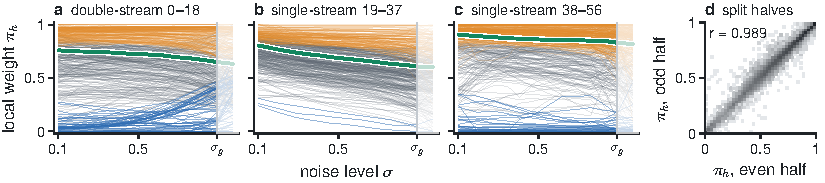
\includegraphics[width=\linewidth]{figures/pi_heads.pdf}
  \caption{\textbf{Heads want different mixes.} (a--c)~$\pi_h(\sigma)$ of all 1368 heads at emulated scale 2; amber: mean above 0.8, blue: below 0.2, green: median; $\sigma>\sigma_g$ veiled. (d)~Tables from disjoint prompt halves agree ($r=0.989$).}
  \label{fig:pi_heads}
\end{figure}

\paragraph{Statistics.} For every emulated scale, block, head, and noise bin, the pass stores $A$, $B$, $E$, the error of the local branch alone $\sum\|\Ofull-\Oloc\|^2$, $\sum\|\Ofull\|^2$, and the query count, in float64, summed over image queries and channels (\texttt{sca/calib.py}). The sampler's trajectory is that of unmodified full attention; the emulated operators only observe. Statistics are written per prompt and merged by summation, so prompts can be added later and split-half fits need no extra pass. Text-query outputs are not in the objective, because \sca{} sends text queries through the global branch only.

\paragraph{Geometry at emulated scale.} At $1024^2$ the grid is $64\times64$. Emulated scale 2 uses a $32\times32$ window, $2\times2$ subsampling onto a $32\times32$ grid, and $4\times4$ query tiles; emulated scale 4 uses a $16\times16$ window, $4\times4$ subsampling onto a $16\times16$ grid, and $2\times2$ tiles. At $1280^2$ the grid is $80\times80$, and emulated scale 2 uses a $40\times40$ window, $2\times2$ subsampling onto a $40\times40$ grid, and $5\times5$ tiles.

\paragraph{Noise bins.} With 28 steps and $\mu=1.15$, $\sigma$ runs from 1.0 to 0.105, so the lowest of the 14 bins is empty and copies its neighbour; 13 bins are populated. Under this schedule 8 steps have $\sigma>0.89$ (the ninth has $\sigma=0.888$) and 13 have $\sigma>0.80$.

\begin{figure}[!htbp]
  \centering
  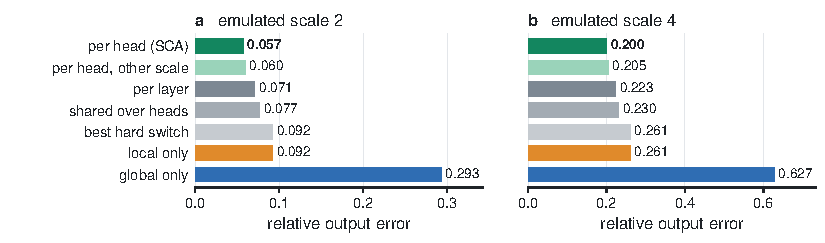
\includegraphics[width=\linewidth]{figures/rel_err.pdf}
  \caption{\textbf{Per-head weights explain full attention best, and transfer across scales.} Relative output error per mixing rule at emulated scales 2 (a) and 4 (b), 32 prompts; ``other scale'' swaps the scale-2 and scale-4 tables; the best hard switch ($\sigma^\star = 1$) equals local only. In-sample and held-out errors agree within 0.0003.}
  \label{fig:relerr}
\end{figure}

\begin{figure}[!htbp]
  \centering
  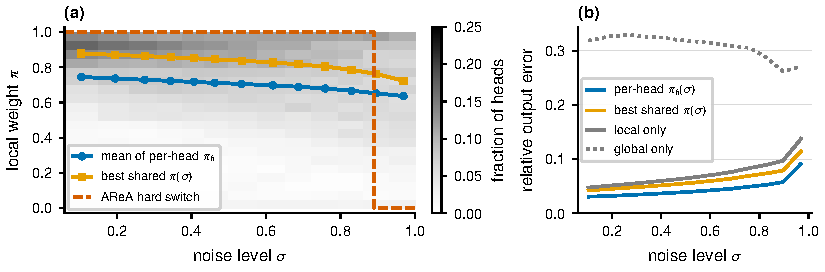
\includegraphics[width=\linewidth]{figures/pi_sigma.pdf}
  \caption{\textbf{In output energy, no noise level prefers the global branch.} (a)~Fraction of heads per $\pi$ and noise bin, with mean $\pih$, best shared $\pi(\sigma)$ and AReA's switch; scale 2, 32 prompts, $\sigma = 1$: pure noise. (b)~Error per noise bin: local beats global everywhere; per-head mixing beats both.}
  \label{fig:pisigma}
\end{figure}

\paragraph{No global phase in output energy.} The best single shared weight falls from 0.88 at $\sigma=0.10$ to 0.72 at $\sigma=0.97$, and the mean per-head weight from 0.74 to 0.64 (Figure~\ref{fig:pisigma}); within a block, the per-head weights span a median range of 0.66 to 0.84 at every noise level (Figure~\ref{fig:heatmap}). Among hard switches from global to local, the best threshold is $\sigma^\star=1$, which equals local only. A switch at $\sigma^\star=0.89$ between our two branches raises the error from 0.092 to 0.152 at scale 2 and from 0.261 to 0.376 at scale 4. In the noisiest bin, the global branch alone has relative error 0.27 at scale 2, the local branch alone 0.14, and the per-head mix 0.09. The generation results of Section~\ref{sec:ablations} show the opposite preference for the opening steps, which is the gap between squared output error and layout.

\paragraph{Attention mass.} For 256 random image queries per block and step, the pass also records the softmax mass on text keys and on image keys within Chebyshev distance 2, 4, 8, and 16. At $1024^2$, averaged over heads and queries, text receives 15 to 19\% of the mass; image keys within distance 16 receive 52\% at $\sigma=0.10$ and 40\% at $\sigma=0.97$, and keys outside that $33\times33$ neighbourhood still receive 29\% and 41\%. A purely local receptive field cannot account for any step, even at native resolution. Figure~\ref{fig:heads}b and~d use the per-head shares in the noise bin at $\sigma=0.62$; panel b caps the opacity at 12 times the uniform density, which clips only the local head's core.

\paragraph{Calibration budget.} We merge the stored sufficient statistics from the first 4, 8, or 16 calibration prompts and rerun the \nabl{} ablation prompts with each resulting table. Table~\ref{tab:phase2_sensitivity} reports generation-level differences from the 32-prompt table. The test reuses calibration observations but uses separate prompts for generation evaluation; it is not a held-out output-error benchmark.

\begin{figure}[!htbp]
  \centering
  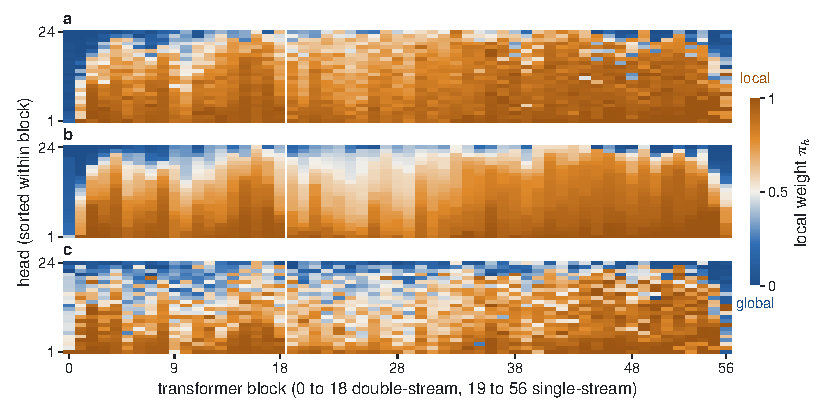
\includegraphics[width=\linewidth]{figures/pi_heatmap.pdf}
  \caption{\textbf{Heads in the same block differ widely at every noise level.} $\pih$ of the scale-2 table at $\sigma = 0.10$ (a), $0.54$ (b), $0.97$ (c), 57 blocks by 24 heads, 32 prompts, heads sorted per block by (b). Median within-block range 0.66 to 0.84; Figure~\ref{fig:calib} shows the scale-4 inference table.}
  \label{fig:heatmap}
\end{figure}

\FloatBarrier
\section{Calibration prompts}
\label{app:prompts}

This section lists the prompts behind the calibration of Section~\ref{sec:analysis} and Algorithm~\ref{alg:calib} (\texttt{scripts/calib\_prompts.jsonl}). The $1024^2$ table uses prompts 1 to 32 and the $1280^2$ table prompts 1 to 16. None of them is an evaluation prompt.

{\scriptsize
\begin{multicols}{2}
\begin{enumerate}[leftmargin=1.6em,itemsep=0pt,topsep=0pt,parsep=0pt]
  \item A candid street portrait of an elderly fisherman with a weathered face and a knitted wool cap, harbor in the background, overcast light
  \item Two children laughing while running through a lawn sprinkler on a summer afternoon, backlit by the sun
  \item A professional headshot of a young woman with curly red hair and freckles, soft studio lighting, neutral grey backdrop
  \item A jazz trio performing in a dim basement club, saxophone player in the foreground, warm stage lights and haze
  \item A chef plating a dessert in a busy restaurant kitchen, steam rising, stainless steel counters
  \item A ballet dancer mid-leap in an empty rehearsal studio with tall windows and wooden floors
  \item A red fox standing in fresh snow at the edge of a birch forest, early morning light
  \item A macro photograph of a honeybee covered in pollen on a purple lavender flower
  \item A herd of elephants crossing a dusty savanna river at sunset, long shadows
  \item A tabby cat sleeping curled up on a stack of old books next to a window
  \item A school of tropical fish swimming around a coral reef, sun rays through clear blue water
  \item A bald eagle perched on a dead pine branch above a misty lake
  \item A neon sign reading ``OPEN 24 HOURS'' in the window of a rainy diner at night, reflections on the wet sidewalk
  \item A hand-painted wooden sign that says ``Fresh Eggs'' leaning against a farm fence, chickens nearby
  \item A vintage movie theater marquee with the words ``NOW SHOWING'' lit by hundreds of bulbs
  \item A chalkboard menu in a cafe listing coffee drinks and prices in neat handwriting
  \item A highway road sign reading ``Exit 42 Pine Valley'' against a clear blue sky
  \item A bookstore storefront with gold lettering ``Second Chapter Books'' on the glass, autumn leaves on the ground
  \item A wide alpine valley with a winding river, snow-capped peaks and wildflower meadows, midsummer
  \item Sand dunes in the desert at golden hour with sharp ridges and wind ripples
  \item A rugged coastline with sea stacks and crashing waves under a stormy sky
  \item A terraced rice field on a hillside in morning fog, farmers in conical hats
  \item The northern lights over a frozen lake with a small wooden cabin, stars visible
  \item A dense tropical rainforest with a waterfall and hanging vines, light filtering through the canopy
  \item A cozy Scandinavian living room with a fireplace, sheepskin rug, and large windows showing snow outside
  \item A modern open-plan kitchen with a marble island, pendant lights, and potted herbs
  \item A cluttered artist studio with canvases, paint tubes, brushes in jars, and afternoon sunlight
  \item A grand library reading room with long oak tables, green lamps, and arched ceilings
  \item A small Japanese tatami room with a low table, sliding paper doors, and a garden view
  \item A product photograph of a matte black wristwatch on a slate surface, dramatic side light
  \item A pair of white running shoes floating against a pastel gradient background, studio product shot
  \item A glass bottle of olive oil with a sprig of rosemary on a rustic wooden table, soft daylight
  \item A flat lay of a leather notebook, fountain pen, glasses, and a cup of espresso on a desk
  \item A ceramic teapot with a blue glaze and matching cups arranged on a linen tablecloth
  \item A crowded night market in Taipei with food stalls, lanterns, and hundreds of people
  \item A packed football stadium during a night match, floodlights and cheering fans
  \item Commuters crossing a huge intersection in Tokyo during rush hour, seen from above
  \item A music festival crowd at sunset with raised hands and confetti in the air
  \item A busy train station concourse with travelers, departure boards, and a glass roof
  \item A gothic cathedral facade with intricate stone carvings and a rose window, low angle
  \item A row of colorful Victorian townhouses on a hilly street with a cable car
  \item A brutalist concrete apartment block with repeating balconies under a pale sky
  \item A glass skyscraper reflecting clouds, shot looking straight up from the street
  \item A traditional Chinese pagoda beside a lake with cherry blossoms in full bloom
  \item An old stone bridge over a canal in Venice with gondolas and laundry lines
  \item An astronaut riding a horse across a red desert planet with two moons, cinematic
  \item A detailed watercolor illustration of a lighthouse on a rocky island with seagulls
  \item A steampunk airship floating above a Victorian city at dusk, intricate brass details
\end{enumerate}
\end{multicols}}

\FloatBarrier
\section{Implementation details and cost}
\label{app:impl}

This section expands Section~\ref{sec:branches} and Figure~\ref{fig:method}. Figure~\ref{fig:method_zoom} draws the two operators, the gate, and the mix at component level, together with the calibrated table for all 57 blocks. Table~\ref{tab:flops} gives attention cost, and Table~\ref{tab:latency} and Figure~\ref{fig:latency_full} end-to-end latency; Appendix~\ref{app:code} writes out the corresponding algorithms.

\begin{figure}[t]
  \centering
  \IfFileExists{figures/method_zoom.pdf}{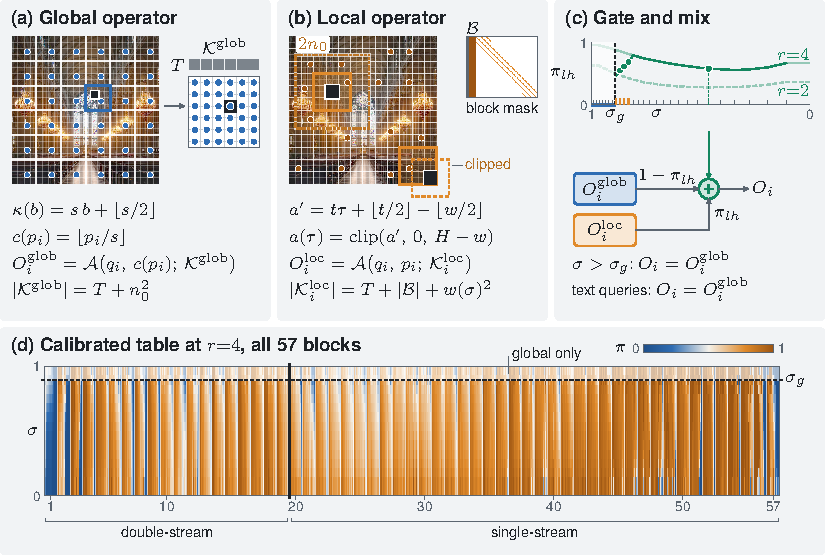
\includegraphics[width=\linewidth]{figures/method_zoom.pdf}}{\fbox{\parbox{0.9\linewidth}{\centering method\_zoom.pdf pending}}}
  \caption{\textbf{The operators at component level.} (a)~The global operator keeps the centre token $\kappa(b)$ of each $s\times s$ block as a key at coarse position $b$ and places query $i$ at $c(p_i)$ (Equation~\ref{eq:glob}). (b)~Each $t\times t$ query tile attends in one softmax to the text keys, the bridge set $\mathcal{B}$ (dots; Equation~\ref{eq:bridge}) and a window at original positions, clipped at the border (dashed: unclipped $a'$), whose side shrinks from $2n_0$ (dotted) to $n_0$ after the gate (Equation~\ref{eq:sched}); inset: block mask at $w=n_0$ (grey: text, dark amber: bridge; Equation~\ref{eq:loc}). (c)~Block 2, head 8 (chosen for a large gap; median 0.05) at $r=2$ (dashed) and $r=4$ (solid): window steps (amber ticks) read $\pi_{lh}$ at $r=\max(H,W)/w$, native steps at $r=4$; for $\sigma>\sigma_g$ every head returns $\Oglob_i$ (Equation~\ref{eq:mix}). (d)~The $r=4$ table, all $57\times24$ heads. Toy grid: $H=24$, $s=4$, $n_0=6$, $t=2$, one schematic bridge token per $6\times6$ cell.}
  \label{fig:method_zoom}
\end{figure}

\paragraph{FlexAttention window.} Image tokens are reordered tile-major, so that a sparse block is a small spatial tile. Query blocks cover $8\times16$ tokens (128 queries) and key blocks $8\times8$ (64 keys), shifted so that unclamped windows start on a block edge; text keys come first. The mask function states window membership per query-key pair, so the result does not depend on the block layout, only the amount of skipped work does. On GH200, $8\times16$ query blocks with $8\times8$ key blocks were fastest at $2048^2$, $4096^2$, and $2048\times6144$. RoPE, subsampling, both branches, and the mix compile into one graph per layer; the mix is in fp32.

\paragraph{Numerical checks.} The 18 CPU tests in \texttt{tests/test\_sca.py} use float32 to check full-mode agreement with stock FLUX attention, both branches against brute-force Equations~\ref{eq:glob} and~\ref{eq:loc}, full-grid and factor-1 identities, calibration when the local branch is exact, the gate, and FlexAttention against an explicit gather reference. A separate GPU check in \texttt{scripts/bench\_attn.py} compares the gather and FlexAttention implementations in bf16: the recorded maximum absolute difference is 0.015625, and both have the same maximum error against the fp32 reference on the tested grids. This is an observed absolute-error check; no per-element ULP bound was measured.

\paragraph{Position ids in bf16.} The FLUX.1 pipeline builds image position ids in bf16, which cannot represent every integer above 256. Our frozen runs retain these rounded ids for RoPE. Passing the true grid from the sampler fixes window membership and subsampling geometry, but does not restore exact RoPE coordinates: the coarse-query positions are also computed from the rounded ids. At a 384-token axis, index 383 rounds to 384 and its scale-6 coarse coordinate becomes 64; at a 512-token axis, index 511 rounds to 512 and its scale-8 coarse coordinate also becomes 64. A local 64-token window can likewise have a rounded endpoint difference of 64 instead of the ideal bound 63. Proposition~\ref{prop:range} therefore applies exactly to the mathematical operator, not to these finite-precision positions at $2048\times6144$, $6144^2$, or $8192^2$. The $4096^2$ grid uses indices 0--255, which bf16 represents exactly. FLUX.2 uses integer position ids. Rebuilding FLUX.1 positions in higher precision would require a separate controlled experiment; the reported runs are unchanged.

\paragraph{Non-divisible grids.} When $H/n_0$ is not an integer, the subsampling factor per axis is the divisor of $H$ nearest to $H/n_0$, and the tile side the divisor nearest to $t$; neither case arises at the sizes we evaluate.

\begin{table}[!htbp]
  \caption{\textbf{Cost.} Top: analytic attention FLOPs per image (57 blocks, 24 heads, head dimension 128, 28 steps, $T=512$); ``gated'' skips the local branch in the first 8 steps; ratio is full over gated \sca{}. Bottom: measured time of one attention layer in bf16 on GH200, minimum over interleaved runs; \sca{} is both branches and the mix.}
  \label{tab:flops}
  \centering
  \small
  \setlength{\tabcolsep}{4pt}
  \begin{tabular}{lcccccc}
    \toprule
    Size ($H\times W$) & Grid & $(s_H,s_W)$ & Full & \sca{}, no gate & \sca{}, gated & Ratio \\
    \midrule
    $2048\times4096$ & $128\times256$ & (2, 4) & $2.17\times10^{16}$ & $5.97\times10^{15}$ & $5.12\times10^{15}$ & 4.2 \\
    $4096\times4096$ & $256\times256$ & (4, 4) & $8.56\times10^{16}$ & $1.19\times10^{16}$ & $1.02\times10^{16}$ & 8.4 \\
    $2048\times6144$ & $128\times384$ & (2, 6) & $4.84\times10^{16}$ & $8.93\times10^{15}$ & $7.66\times10^{15}$ & 6.3 \\
    \midrule
    Token grid & \multicolumn{2}{c}{Pixels} & Full (SDPA, ms) & \multicolumn{2}{c}{\sca{} (ms)} & Speedup \\
    \midrule
    $128\times128$ & \multicolumn{2}{c}{$2048^2$} & 7.1 & \multicolumn{2}{c}{5.2} & 1.4 \\
    $256\times256$ & \multicolumn{2}{c}{$4096^2$} & 87.3 & \multicolumn{2}{c}{18.7} & 4.7 \\
    $128\times384$ & \multicolumn{2}{c}{$2048\times6144$} & 49.6 & \multicolumn{2}{c}{14.0} & 3.5 \\
    \bottomrule
  \end{tabular}
\end{table}

\begin{table}[!htbp]
  \caption{\textbf{Seconds per image}, batch 1, idle GH200, 28 steps with text encoding and VAE decoding, median of three timed images after an excluded warm-up; full attention not run at $8192^2$.}
  \label{tab:latency}
  \centering\footnotesize
  \setlength{\tabcolsep}{8pt}
  \begin{tabular}{lrrr}
    \toprule
    Size ($N$ tokens) & Full attention & AReA & \sca{} \\
    \midrule
    $2048^2$ (16{,}384) & 22.9 & 41.0 & \textbf{18.2} \\
    $3072^2$ (36{,}864) & 73.9 & 114.3 & \textbf{40.2} \\
    $4096^2$ (65{,}536) & 186.5 & 202.4 & \textbf{71.1} \\
    $6144^2$ (147{,}456) & 762.7 & 482.3 & \textbf{161.6} \\
    $8192^2$ (262{,}144) & not run & 952.0 & \textbf{287.6} \\
    \bottomrule
  \end{tabular}
\end{table}

\begin{figure}[!htbp]
  \centering
  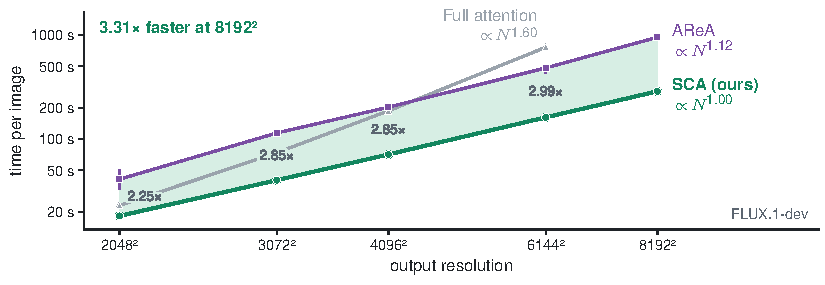
\includegraphics[width=\linewidth]{figures/latency.pdf}
  \caption{\textbf{Latency at every size.} Figure~\ref{fig:latency} at full width: batch 1 on one GH200, median of three prompts, whiskers min to max; full attention was not run at $8192^2$. Grey ratios: speedup over AReA per size; exponents fit seconds $\propto N^b$ ($N$ image tokens).}
  \label{fig:latency_full}
\end{figure}

\paragraph{End-to-end latency.} Table~\ref{tab:latency} and Figure~\ref{fig:latency_full} come from one matched protocol on one GH200 (\texttt{results/\allowbreak latency\_curve\_batch1.csv}, which also lists the excluded warm-up images; \texttt{results/\allowbreak latency\_curve\_summary.csv} summarizes all cells but full attention at $6144^2$). At each size, each method generates one excluded warm-up image and then three timed images in the same process, at batch 1 and 28 steps; we report the median. At $4096^2$ the medians are 186.5\,s for full attention (186.0, 186.6, 186.5), 202.4\,s for AReA (192.7, 202.4, 204.3), and 71.1\,s for \sca{} (71.0, 71.1, 71.1). At $2048^2$ and $3072^2$ they are 22.9 and 73.9\,s for full attention, 41.0 and 114.3\,s for AReA, and 18.2 and 40.2\,s for \sca{}. At $6144^2$ and $8192^2$, AReA takes 482.3 and 952.0\,s and \sca{} 161.6 and 287.6\,s, so \sca{} reduces measured time by 66.5\% and 69.8\%. At $6144^2$ full attention takes 762.7\,s (763.5, 762.7, 762.5), $4.7\times$ \sca{}'s time. An earlier $4096^2$ benchmark, kept as a separate repeat (\texttt{results/\allowbreak latency\_4096\_batch1.csv}), gave 184.6\,s for full attention (184.1, 184.7, 184.6), 212.6\,s for AReA (207.3, 225.8, 212.6), 88.1\,s for \sca{} + band guard (88.1, 98.7, 88.1; single-pass compiled band), and 71.0\,s for \sca{} final (71.0, 83.1, 70.9). On the shared campaign nodes, in the 191-prompt run that also timed the band guard, per-image times at $4096^2$ were 71\,s for \sca{} final, 120\,s for \sca{} + band guard, and 262\,s for AReA; the campaign code used an unfused band, so dropping it saved more there (49\,s) than in the clean measurement (17\,s). At the non-square sizes we have only campaign timings, with both methods on the same pool of shared nodes (mean over \nmain{} prompts): \sca{} takes 38.1\,s and AReA 112.4\,s at $2048\times4096$, and 55.8\,s and 150.5\,s at $2048\times6144$.

\FloatBarrier
\clearpage
\section{Algorithms in full}
\label{app:code}

Algorithms~\ref{alg:calib_full} and~\ref{alg:sample_full} expand Algorithms~\ref{alg:calib} and~\ref{alg:sample} to every step the code performs, and Algorithm~\ref{alg:prog} gives progressive \sca{} (Section~\ref{sec:progressive}). Each step follows \texttt{sca/calib.py}, \texttt{sca/attn.py}, or \texttt{scripts/sample\_progressive.py} in the code repository (link in the abstract), and each comment names the equation or setting that a line implements.

\noindent\begin{minipage}[t]{0.48\linewidth}
    \hrule height 0.6pt\vspace{2pt}
    \captionof{algorithm}{\textbf{Calibration}, in full}
    \label{alg:calib_full}
    \vspace{-4pt}
\begin{lstlisting}[style=scacode, emph={bin,on_step,calibrate,attn,global_branch,local_branch,sample,clip,where,arange,fill_empty_bins}]
# Input: 32 prompts; FLUX.1-dev at (*@$1024^2$@*) (n = 64),
#   28 steps, guidance 4.5, full attention
# Output: pi[s_c, l, h, beta], centres[beta]
def bin(sigma): return min(int(14 * sigma), 13)
def on_step(sigma):          # once per step
  S[bin(sigma)] += sigma; C[bin(sigma)] += 1
def calibrate(q, k, v, l, sigma):  # every block
  O_full = attn(q, k, v)     # Eq. (*@\ref{eq:attn}@*), all keys
  beta = bin(sigma)          # 14 bins, width 1/14
  for s_c in (2, 4):         # emulation, App. (*@\ref{app:calib}@*)
    f, w = s_c, n // s_c     # subsample, window
    t_c = round(t * w / n0)  # tile sides 4 and 2
    O_glob = global_branch(q, k, v, f)    # Eq. (*@\ref{eq:glob}@*)
    O_loc = local_branch(q, k, v, w, t_c) # Eq. (*@\ref{eq:loc}@*)
    dl, df = O_loc - O_glob, O_full - O_glob
    # Eq. (*@\ref{eq:stats}@*): per head, over image rows, channels
    A[s_c, l, :, beta] += sum(dl * dl)
    B[s_c, l, :, beta] += sum(df * dl)
    E[s_c, l, :, beta] += sum(df * df)
    F[s_c, l, :, beta] += sum(O_full * O_full)
  return O_full              # sampler unchanged
sample(prompts, on_step, calibrate)
pop = C > 0                  # 13 of 14 bins
centres = where(pop, S / C, (arange(14)+0.5)/14)
pi = clip(B / A, 0, 1); pi[A == 0] = 1  # Prop. (*@\ref{prop:opt}@*)
pi = fill_empty_bins(pi, pop)  # nearest bin
J = E - 2 * pi * B + pi**2 * A # error of the mix
rel_err = J.sum() / F.sum()    # Section (*@\ref{sec:analysis}@*)
\end{lstlisting}
\end{minipage}\hfill
\begin{minipage}[t]{0.48\linewidth}
    \hrule height 0.6pt\vspace{2pt}
    \captionof{algorithm}{\textbf{Sampling}, in full}
    \label{alg:sample_full}
    \vspace{-4pt}
\begin{lstlisting}[style=scacode, emph={rope,sdpa,cat,clip,log2,interp,top_k,tile_major,block_mask,flex_attention,inverse}]
# Input: q, k, v before RoPE (T text, then H x W
#   image), block l, noise level sigma
# Output: O for all T + HW queries; sca/attn.py
# Per image: s_H, s_W = H // n0, W // n0; pi_s is
#   the table entry nearest max(s_H, s_W) in log
# Per step, all 57 x 24 heads, ends held:
w = n0                        # Eq. (*@\ref{eq:sched}@*)
for sig_k, w_k in ((.88, 128), (.86, 112),
                   (.84, 96), (.82, 80)):
  if sigma > sig_k: w = w_k; break
if w == n0: pi = interp(sigma, centres, pi_s)
else:                 # ratio r, log-linear
  r = max(H, W) / w; u = clip(log2(r / 2), 0, 1)
  pi = (1-u) * interp(sigma, centres, table[2]) \
     + u * interp(sigma, centres, table[4])
kb = k_img[s_H//2::s_H, s_W//2::s_W]  # (*@$\kappa(b)$@*)
vb = v_img[s_H//2::s_H, s_W//2::s_W]
cp = p // (s_H, s_W)          # (*@$c(p_i)$@*); text at 0
Q = cat(rope(q_txt, 0), rope(q_img, cp))
K = cat(rope(k_txt, 0), rope(kb, b))
O_glob = sdpa(Q, K, cat(v_txt, vb))   # Eq. (*@\ref{eq:glob}@*)
if sigma > sigma_g:                   # 0.89, Eq. (*@\ref{eq:mix}@*)
  return O_glob               # opening phase
# bridge (Eq. (*@\ref{eq:bridge}@*)), per block and step:
d = ((k_img - k_img.mean(0))**2).sum(heads, ch)
B = top_k(d, 16) per cell, 8 x 8 cells  # 1,024
kr = rope(k_img, p)           # true positions
kl = cat(rope(k_txt, 0), kr[B], kr)
vl = cat(v_txt, v_img[B], v_img)  # no dedup
P = T + len(B)                # prefix, seen by all
w = (min(w, H), min(w, W))    # window sides
a = clip(t*(p//t) + t//2 - w//2, 0, (H, W) - w)
keep(i, j) = j < P or a_i <= p_j < a_i + w  # Eq. (*@\ref{eq:loc}@*)
perm = tile_major(H, W)       # 8 x 16 query blocks
mask = block_mask(keep, perm) # 8 x 8 key blocks
O_loc = flex_attention(rope(q_img, p)[perm],
    kl, vl, mask)[inverse(perm)]
O_img = pi[l] * O_loc + (1 - pi[l]) * O_glob[T:]
return cat(O_glob[:T], O_img) # fp32 mix, Eq. (*@\ref{eq:mix}@*)
\end{lstlisting}
\end{minipage}

\vspace{10pt}
\noindent\begin{minipage}{\linewidth}
    \hrule height 0.6pt\vspace{2pt}
    \captionof{algorithm}{\textbf{Progressive \sca{}}, HRDiT's schedule with \sca{} attention (Section~\ref{sec:progressive})}
    \label{alg:prog}
    \vspace{-4pt}
\begin{lstlisting}[style=scacode, emph={shift,linspace,noise,flux,decode,encode,bicubic,sharpen,lowpass,up,momentum,use_sca}]
# Input: prompt, seed; FLUX.1-dev in bf16; SCA tables at scales 2 and 4
# Output: (*@$4096^2$@*) image; scripts/sample_progressive.py
sig = shift(linspace(1, 1/30, 30), mu=1.15)     # one 30-step schedule serves all stages, as in HRDiT
x = noise((*@$1024^2$@*), seed)                         # stage 1: stock dense attention, native RoPE
for i in range(30):                             # Euler; ref keeps each step's x0 estimate
  v = flux(x, sig[i], g=3.5); ref[i] = x - sig[i] * v; x = x + (sig[i+1] - sig[i]) * v
for res, k, g, s_c, a in ((2048, 13, 4.5, 2, 1.0), (4096, 20, 6.0, 4, 0.25)):
  img = sharpen(bicubic(decode(x), res))        # 2 img - blur(img), blur width ~ U(0.1, 2.0)
  x = sig[k] * noise + (1 - sig[k]) * encode(img)   # re-enter at sigma 0.81, then 0.61
  use_sca(table[s_c], n0=64, t=8, sigma_g=0.89, bridge=(8, 16))  # replaces NTK RoPE, attention scale,
                                                # pruning, alignment; w = n0, as sig[k] < 0.82 (Eq. (*@\ref{eq:sched}@*))
  N = 30 - k                                    # 17, then 10 steps; sig[k] < sigma_g: no opening phase
  for n, i in enumerate(range(k, 30)):
    v = flux(x, sig[i], g); x0 = x - sig[i] * v; r, ref[i] = ref[i], x0    # SCA in every block
    x0 = x0 + a * (N - n) / N * (lowpass(up(r)) - lowpass(x0))  # Butterworth, order 4, cut-off 0.2
    u = momentum((x - x0) / sig[i], 0.5 * (N - n) / N)           # HRDiT's velocity momentum
    x = x + (sig[i+1] - sig[i]) * u
return decode(x)
\end{lstlisting}
\end{minipage}

\FloatBarrier
\section{Hyperparameters}
\label{app:hparams}

Table~\ref{tab:hparams} expands the Models and hyperparameters paragraph of Section~\ref{sec:experiments} and lists every setting of the main runs.

\begin{table}[!htbp]
  \caption{\raggedright\textbf{All hyperparameters} of the main runs (code commit \texttt{7bd64c0}), produced by \texttt{scripts/sample.py -{}-method sca -{}-pi-table calib/k1\_1024.npz -{}-gate-sigma 0.89 -{}-bridge-cells 8 -{}-bridge-k 16 -{}-win-sched 0.88:128,0.86:112,0.84:96,0.82:80 -{}-win-pi-match -{}-win-pi-interp}. Appendix~\ref{app:additional_protocols} gives the settings that differ for UltraImage, HRDiT, SigMa, and FLUX.2-dev.}
  \label{tab:hparams}
  \centering\footnotesize
  \setlength{\tabcolsep}{4pt}
  \begin{tabular}{@{}ll>{\raggedright\arraybackslash}p{0.52\linewidth}@{}}
    \toprule
    Group & Setting & Value \\
    \midrule
    Model & checkpoint, precision & FLUX.1-dev, bf16 weights and activations \\
     & blocks, heads, head dim & 19 double-stream + 38 single-stream, 24, 128 \\
     & native grid $n_0$, text tokens $T$ & 64 ($1024^2$ pixels, 16 pixels per token), 512 \\
    Sampler & steps, solver & 28, flow-matching Euler \\
     & guidance, shift & 4.5 (distilled guidance), $\mu=1.15$ at every size \\
     & seed, decoding & seed 0 per prompt, shared across methods; tiled VAE decoding \\
    Local branch & tile $t$ & 8 \\
     & window $w(\sigma)$ & 128, 112, 96, 80 for $\sigma$ in $(0.88,0.89]$, $(0.86,0.88]$, $(0.84,0.86]$, $(0.82,0.84]$, then 64; clamped at borders; original positions \\
     & bridge & 16 tokens per cell of an $8\times8$ grid (1,024), farthest from the mean key, recomputed per block and step, true positions \\
     & kernel & FlexAttention; query blocks $8\times16$, key blocks $8\times8$, tile-major order \\
    Global branch & subsampling & block centre, factor $(s_H,s_W)$ = target grid / $n_0$ \\
     & positions & queries at $c(p)$, keys at block index, text at 0 \\
    Mixing & table & per (block, head, $\sigma$ bin, ratio), $57\times24\times14\times2$, ratios 2 and 4 \\
     & ratio & $r=\max(H,W)/w(\sigma)$, weight linear in $\log_2 r$ between ratios 2 and 4, nearest outside \\
     & interpolation & linear in $\sigma$ between the mean sampled noise levels of occupied bins, constant outside \\
     & gate & $\sigma_g=0.89$ (8 of 28 steps global only, then 4 wide-window steps) \\
    Calibration & prompts, resolution & 32 at $1024^2$ (16 more at $1280^2$ for transfer) \\
     & emulated scales & 2 and 4, one pass; 14 bins of width $1/14$ \\
     & hardware & one GH200; complete calibration runtime was not retained \\
    Band guard & (not in final method) & average-pool $p=16$, bilinear upsampling \\
    \bottomrule
  \end{tabular}
\end{table}

\FloatBarrier
\section{Evaluation protocol and metrics}
\label{app:metrics}

This section expands the Data and Metrics paragraphs of Section~\ref{sec:experiments}: Table~\ref{tab:protocol} summarizes the protocol, and the paragraphs below define each metric and interval.

\begin{table}[!htbp]
  \caption{\textbf{Evaluation protocol.} The FLUX.1-dev attention comparisons share sampler settings and prompt seeds. UltraImage and HRDiT use their own multi-stage protocols; FLUX.2-dev uses its own native-resolution schedule (Appendix~\ref{app:additional_protocols}). \ifmainfull{Prompt counts include the four development prompts.}{Prompt counts exclude the four development prompts.} Table~\ref{tab:hparams} lists the hyperparameters; the paragraphs below define the metrics.}
  \label{tab:protocol}
  \centering\footnotesize
  \setlength{\tabcolsep}{4pt}
  \begin{tabular}{@{}p{0.13\linewidth}p{0.83\linewidth}@{}}
    \toprule
    Models & FLUX.1-dev~\citep{flux2024} (main results); FLUX.1-Krea-dev~\citep{krea2025flux} (\nkrea{} prompts); FLUX.2-dev~\citep{flux2_2025} (50 prompts); bf16. \\
    Sampler & 28 Euler flow-matching steps, guidance 4.5, shift $\mu=1.15$ at every size, seed label 0 per prompt, tiled VAE decoding; UltraImage, HRDiT, and FLUX.2-dev exceptions are detailed in Appendix~\ref{app:additional_protocols}. \\
    Sizes & $4096^2$, $2048\times4096$, $2048\times6144$ (\nmain{} prompts each); $6144^2$ (100-prompt subset); $8192^2$ (12 exploratory paired prompts, metrics and qualitative examples). \\
    Prompts & Aesthetic-4K evaluation set with 4K references~\citep{zhang2025diffusion4k}, \nmain{} prompts, fixed \nabl-prompt ablation subset; HRGen-1K~\citep{rajabi2026area}, \ifhrgenfull{all 1000 prompts}{\nhrgen{} of 1000 prompts}. \\
    Baselines & Full attention; AReA, released code~\citep{rajabi2026area}; DyPE~\citep{issachar2025dype}, SEGA~\citep{rajabi2026sega}, UltraImage~\citep[two-stage defaults;][]{zhao2025ultraimage}, HRDiT~\citep[released progressive protocol;][]{xue2026hrdit}; SigMa~\citep{zhao2026sigma} on \npanel{} prompts. \\
    Metrics & ImageReward, HPSv2/2.1, PickScore, CLIP, aesthetic; FID, KID, IS, patch FID/KID; MUSIQ (full, $1024^2$ crops), CLIP-IQA, ARNIQA; 95\% paired bootstrap intervals over prompts. \\
    Hardware & One NVIDIA GH200 per process; verified timing logs identify the GH200 120\,GB model. Clean latency uses batch 1; campaign timings are marked separately. \\
    \bottomrule
  \end{tabular}
\end{table}

\paragraph{Prompts and references.} The Aesthetic-4K evaluation split~\citep{zhang2025diffusion4k} has 195 prompts with 4K reference images. Four of them (\devprompts) were used to choose the opening phase and window\ifmainfull{; they stay in the evaluation set for every method, which favours \sca{} slightly}{ and are excluded from generation evaluation, leaving \nmain}. The 195 reference rows hold 168 distinct images (27 duplicate rows, each with its own caption); distribution metrics keep the official rows and weights, as Diffusion-4K's statistics do. The \nabl-prompt ablation subset was fixed before any ablation was run. HRGen-1K~\citep{rajabi2026area} has 1000 prompts and no references; \ifhrgenfull{we use all of them}{we use source rows 0--199, with ids \texttt{hrgen\_0000}--\texttt{hrgen\_0199}}. The 48 calibration prompts were written for this purpose and share no prompt with Aesthetic-4K (the largest word-set Jaccard overlap with any evaluation prompt is 0.26).

\paragraph{Implementations.} torch-fidelity 0.3.0, pyiqa 0.1.16 (MUSIQ) and 0.1.15 (CLIP-IQA, ARNIQA), hpsv2 1.2.0, and image-reward 1.5.

\paragraph{Preference and alignment metrics.} ImageReward v1.0~\citep{xu2023imagereward} (bicubic resize to 224, centre crop). HPSv2 and HPSv2.1~\citep{wu2023hpsv2}: cosine of normalized image and text features with the official validation transform (longest side 224, padded). PickScore~\citep{kirstain2023pickapic}: $\exp(\text{logit scale})$ times the cosine. CLIP score~\citep{radford2021clip}: $100\max(\cos,0)$ with ViT-L/14. Aesthetic: the LAION improved aesthetic predictor (sac+logos+ava1, linear MSE) on the L2-normalized CLIP ViT-L/14 image embedding~\citep{schuhmann2022aesthetic}.

\paragraph{No-reference quality.} MUSIQ~\citep{ke2021musiq} (pyiqa defaults) on the full image at native resolution, and MUSIQ$_\text{c}$, its mean over four fixed random $1024^2$ crops per image; crop positions depend only on the prompt id, so they are identical across methods. CLIP-IQA~\citep{wang2022clipiqa} and ARNIQA~\citep{agnolucci2024arniqa} (pyiqa defaults) on the image downscaled with antialiased bicubic resampling to a long side of 1024 pixels, the scale both were trained on.

\paragraph{Distribution metrics and reference correction.} FID~\citep{heusel2017fid} and KID compare the generated images (\nmain{} on the main set, \npanel{} on the panel) with all 195 official reference rows, using Inception-v3 features (torch-fidelity) after bilinear resizing to $299^2$. The reference rows contain 168 distinct image contents; repeated rows retain their official weights. Patch FID and KID are our own definition: the same Inception features on four fixed random $1024^2$ crops per generated image and per reference row (\the\numexpr4*\nmain\relax{} generated and 780 reference crops on the main set). AReA and SEGA report a patch FID without defining its crops, so patch FID is never compared across papers. An audit found that the original feature-bank assembly keyed reference crops by resolved image path, so repeated images reused the last row's crop features. We corrected the lookup to retain each row's intended cached crops. Whole-image FID/KID are unchanged; all patch point estimates reported here use the corrected assembly. Original CSVs remain archived for provenance. Inception score uses full images at $299^2$, with 10 splits.

\paragraph{Intervals.} Per-image intervals are 95\% paired percentile bootstraps over prompt ids: original summaries use 1000 draws; separately recomputed comparisons use 2000 draws with seed 0. For the main \sca{}--AReA FID/KID and patch-FID/KID comparison, 1000 draws resample generated prompt ids jointly across methods and resample the 168 distinct reference-image identities, keeping all rows and crops from each sampled identity together. This retains the 195-row weighted point estimate while accounting for repeated reference images. The resulting FID difference is $-7.74$ $[-13.11,-2.61]$; patch FID is $-3.79$ $[-7.46,1.29]$ and patch KID ($\times10^3$) is $-2.29$ $[-4.60,0.05]$. An earlier version of this analysis reported a significant patch-KID improvement; under the corrected evaluation its interval includes zero. The whole-image and patch FID/KID comparisons at both non-square sizes, against every added baseline, and for the sampling-budget and progressive runs also use reference-image clusters. Other whole-image FID/KID intervals are labelled historical reference-row bootstraps; they have not been recomputed with image-identity clusters. Historical patch intervals are not attached to corrected estimates and are omitted where recomputation is incomplete. FID's finite-sample bias can place point estimates outside percentile intervals. Intervals are unadjusted for multiple comparisons and measure prompt/reference sampling uncertainty, not variability over independent model training runs.

\FloatBarrier
\section{Reproducing AReA}
\label{app:area}

This section expands the AReA comparison of Section~\ref{sec:main}: our protocol for AReA and our runs beside its published numbers at $4096^2$ (Table~\ref{tab:published_compare}) and on HRGen-1K (Table~\ref{tab:published_hrgen}). We run AReA's released code with its FLUX.1 defaults (block-centre pooling, first phase for 8 of 28 steps, halo width 8, bridge ratio 0.5), the FLUX.1-dev checkpoint, guidance 4.5, 28 steps, $\mu$ at its maximum, and the seeds shared with the other methods. AReA's published numbers match FLUX.1-Krea-dev, the default of its released code: rerunning that code on Krea-dev reproduces its published ImageReward, aesthetic score, and PickScore within 0.1 and its CLIP, HPS, and MUSIQ within 0.3 (Table~\ref{tab:published_compare}), while on FLUX.1-dev the same code gives ImageReward 0.92 against the published 1.32. Our direct \sca{}--AReA comparison holds the FLUX.1-dev settings fixed. UltraImage and FLUX.2-dev use separate protocols (Appendix~\ref{app:additional_protocols}). AReA's paper reports 151\,s for AReA and 314\,s for full attention at $4096^2$ on an H100; the matched sweep measures 202.4\,s and 186.5\,s on one GH200 (medians of three images). We use commit \texttt{9e38ec2} of the released repository, which includes a cost cap on halo and bridge tokens and a jagged halo edge; neither appears in AReA's paper, which does not say whether its Table~1 used them. Recomputed from the code with 512 text tokens, the first-phase pooling factors are 4, 4, 4, 4, 2, 2, 2, 2 at $4096\times4096$ and $2048\times4096$, and 8, 8, 8, 4, 4, 4, 2, 2 at $2048\times6144$. The second-phase windows shrink over 20 steps from 180, 151, and 192 tokens respectively to 64. At $2048\times6144$ no window is cheaper than full attention once the text tokens are counted, so the first window falls back to 192 tokens and the cap drops the bridge and halo on the first three second-phase steps. Other differences from the release defaults are the FLUX.1-dev checkpoint instead of FLUX.1-Krea-dev, and one seed per prompt shared across methods instead of one seed for all prompts. On FLUX.1-Krea-dev, AReA's default checkpoint, we rerun AReA and recalibrate \sca{} (16 prompts at $1024^2$, scale-4 table, other settings unchanged) with the same 28-step, guidance-4.5 sampler on all \nkrea{} prompts; DyPE and SEGA run the Krea transformer through the frozen baseline harness on the 100 prompts of rows 4 to 103. There \sca{} wins six metrics and loses patch FID and, at the edge of significance, ImageReward, at a third of AReA's time (Table~\ref{tab:krea_6144}). Table~\ref{tab:published_hrgen} expands the HRGen-1K block of Table~\ref{tab:published_compare} to every row of AReA's Table~2.
% Generated by results/published_compare/build.py; do not edit by hand.
\begin{table}[t]
  \caption{\textbf{Published numbers at $4096^2$ next to our runs.} Aesthetic-4K, 195 prompts: AReA's Table~1 (HPS and MUSIQ from its Table~6; ``FLUX.1''), our runs with FLUX.1-Krea-dev, the checkpoint AReA's released code uses (28 steps, guidance 4.5), and our FLUX.1-dev protocol. Last block: HRGen-1K (all rows in Table~\ref{tab:published_hrgen}). HPS: HPSv2 $\times100$; MUSIQ on the full image; FID at $299^2$ against the 195 reference rows; patch FID is omitted because AReA does not state its crops. $^\dagger$Fewer than all prompts; not ranked. \textbf{Bold} / \underline{underline}: best / second best among ranked rows (HRGen-1K: bold only); ours shaded. Key result: Our run of AReA's code on FLUX.1-Krea-dev reproduces its published ImageReward, Aesthetic, and PickScore within 0.1 and its CLIP, HPS, and MUSIQ within 0.28; against that run \sca{} is higher on HPS and MUSIQ, within 0.1 on ImageReward, Aesthetic, CLIP, and PickScore, and worse on FID; on HRGen-1K, where we did not rerun AReA on FLUX.1-Krea-dev, \sca{} on that checkpoint exceeds every published AReA score.}
  \label{tab:published_compare}
  \centering\footnotesize
  \setlength{\tabcolsep}{3.2pt}
  \begin{tabular}{@{}lr*{7}{r}@{}}
    \toprule
     & & Image- & Aes- &  & Pick- &  &  &  \\
    Method & $n$ & Reward$\uparrow$ & thetic$\uparrow$ & CLIP$\uparrow$ & Score$\uparrow$ & HPS$\uparrow$ & MUSIQ$\uparrow$ & FID$\downarrow$ \\
    \midrule
    \multicolumn{9}{@{}l}{\emph{Published by AReA, single pass (FLUX.1)}} \\
    Full attention & 195 & $-$0.72 & 5.80 & 25.72 & 20.34 & -- & -- & 179.8 \\
    UltraImage & 195 & $-$0.14 & 6.11 & 26.77 & 20.85 & -- & -- & 169.4 \\
    DyPE & 195 & 1.11 & 6.32 & 28.98 & 22.79 & -- & -- & 155.2 \\
    SigMa & 195 & 1.01 & 6.16 & 28.36 & 22.47 & -- & -- & 156.8 \\
    SEGA & 195 & 1.27 & 6.31 & 29.16 & 23.16 & -- & -- & 150.6 \\
    AReA & 195 & \textbf{1.32} & \underline{6.37} & \textbf{29.71} & \textbf{23.31} & \underline{29.69} & \underline{45.2} & 148.5 \\
    \midrule
    \multicolumn{9}{@{}l}{\emph{Our runs, FLUX.1-Krea-dev, same prompts and metrics}} \\
    AReA & 195 & \underline{1.28} & 6.32 & \underline{29.49} & \underline{23.21} & 29.41 & 45.0 & \textbf{142.6} \\
    DyPE & 100$^\dagger$ & 0.96 & 6.41 & 28.73 & 22.50 & 28.39 & 42.7 & 171.6 \\
    SEGA & 100$^\dagger$ & 1.13 & 6.31 & 29.19 & 23.01 & 29.15 & 46.0 & 164.2 \\
    \rowcolor[HTML]{EAF4F1}\textbf{\sca{} (ours)} & 195 & 1.23 & \textbf{6.39} & 29.41 & 23.20 & \textbf{29.70} & \textbf{46.3} & \underline{144.1} \\
    \midrule
    \multicolumn{9}{@{}l}{\emph{Our runs, FLUX.1-dev, shared sampler}} \\
    AReA & 195 & 0.92 & 6.27 & 27.69 & 22.36 & 28.62 & 39.4 & 145.8 \\
    \rowcolor[HTML]{EAF4F1}\textbf{\sca{} (ours)} & 195 & 1.23 & 6.44 & 29.14 & 23.09 & 29.75 & 45.4 & 138.1 \\
    \midrule
    \multicolumn{9}{@{}l}{\emph{HRGen-1K, 1000 prompts without references: AReA's Table~2 and our FLUX.1-Krea-dev run}} \\
    AReA, published (FLUX.1) & 1000 & 0.60 & 5.87 & 29.89 & 21.44 & 27.50 & -- & -- \\
    \rowcolor[HTML]{EAF4F1}\textbf{\sca{} (ours), FLUX.1-Krea-dev} & 1000 & \textbf{0.78} & \textbf{6.03} & \textbf{30.10} & \textbf{21.64} & \textbf{28.06} & 43.7 & -- \\
    \bottomrule
  \end{tabular}
\end{table}

% Generated by results/published_compare/build.py; do not edit by hand.
\begin{table}[!htbp]
  \caption{\textbf{HRGen-1K: AReA's published Table~2 next to our runs.} All 1000 prompts at $4096^2$, no reference images. Top: AReA's Table~2 (``FLUX.1'', which its released code runs as FLUX.1-Krea-dev). Bottom: \sca{} with a Krea-calibrated table on FLUX.1-Krea-dev (28 steps, guidance 4.5), and our paired FLUX.1-dev runs of AReA and \sca{}. HPS: HPSv2 $\times100$; IS: Inception score; MUSIQ on the full image; $^\dagger$fewer than 1000 prompts. \textbf{Bold} / \underline{underline}: best / second best among the published rows and our FLUX.1-Krea-dev row. Table~\ref{tab:published_compare} holds the Aesthetic-4K comparison. Key result: \sca{} on FLUX.1-Krea-dev exceeds AReA's published ImageReward, Aesthetic, CLIP, PickScore, HPS, and IS.}
  \label{tab:published_hrgen}
  \centering\footnotesize
  \setlength{\tabcolsep}{3.2pt}
  \begin{tabular}{@{}lr*{7}{r}@{}}
    \toprule
     & & Image- & Aes- &  & Pick- &  &  &  \\
    Method & $n$ & Reward$\uparrow$ & thetic$\uparrow$ & CLIP$\uparrow$ & Score$\uparrow$ & HPS$\uparrow$ & IS$\uparrow$ & MUSIQ$\uparrow$ \\
    \midrule
    \multicolumn{9}{@{}l}{\emph{Published by AReA (FLUX.1)}} \\
    Full attention & 1000 & $-$1.46 & 5.12 & 23.36 & 19.04 & 23.20 & 7.2 & -- \\
    UltraImage & 1000 & $-$0.03 & 5.77 & 28.26 & 20.46 & 26.90 & 10.2 & -- \\
    DyPE & 1000 & 0.33 & 5.83 & 29.35 & 20.94 & 26.60 & 10.9 & -- \\
    SigMa & 1000 & 0.06 & 5.63 & 27.91 & 20.54 & 25.80 & 10.7 & -- \\
    SEGA & 1000 & 0.44 & 5.82 & 29.63 & 21.18 & 27.00 & 12.0 & -- \\
    AReA & 1000 & \underline{0.60} & \underline{5.87} & \underline{29.89} & \underline{21.44} & \underline{27.50} & \underline{13.9} & -- \\
    \midrule
    \multicolumn{9}{@{}l}{\emph{Our runs}} \\
    \rowcolor[HTML]{EAF4F1}\textbf{\sca{} (ours), FLUX.1-Krea-dev} & 1000 & \textbf{0.78} & \textbf{6.03} & \textbf{30.10} & \textbf{21.64} & \textbf{28.06} & \textbf{15.7} & 43.7 \\
    AReA, our run, FLUX.1-dev & 1000 & $-$0.03 & 5.92 & 26.08 & 20.43 & 26.16 & 12.7 & 37.4 \\
    \rowcolor[HTML]{EAF4F1}\textbf{\sca{} (ours), FLUX.1-dev} & 1000 & 0.79 & 6.25 & 28.73 & 21.61 & 28.11 & 15.3 & 45.1 \\
    \bottomrule
  \end{tabular}
\end{table}


\FloatBarrier
\section{Other baselines and FLUX.2-dev}
\label{app:additional_protocols}

\paragraph{DyPE and SEGA.} We use the existing baseline harness frozen at commit \texttt{c05ebdc}, with FLUX.1-dev, 28 steps, guidance 4.5, maximum shift, tiled VAE decoding, and the same prompt-derived seeds as \sca{}. These settings isolate the attention/position treatment on the checkpoint used in our main comparison. They do not reproduce the methods' reported FLUX.1-Krea-dev results; on Krea weights both trail AReA on ImageReward (Table~\ref{tab:krea_6144}). Their low FLUX.1-dev scores should therefore not be read as a ranking under each method's preferred checkpoint.

\paragraph{UltraImage.} We run a guided two-stage configuration from the FLUX branch of the released implementation through \texttt{scripts/run\_ultraimage.py}. It uses a $1024^2$ first stage and a $4096^2$ second stage, 30 steps per stage, guidance 3.5 then 7, the \texttt{super\_imax} guidance schedule, shifted-window patchification, proportional attention, RIFLEx positions, and attention decay. Each prompt also needs a 2+2-step block-average preparation pass. The reported campaign time includes preparation when not cached and the two-stage call; main-stage and preparation times are retained separately in sidecars. Each call reseeds both the generator and the global RNG, including the VAE sampling path, from the prompt id and seed label. Thus seed labels are paired, but the two-stage method does not share an identical latent trajectory with the one-stage methods. The wrapper preserves an upstream scheduler behaviour: assigning \texttt{scheduler.config.shift} does not update the scheduler's internal shift in the installed diffusers version, so both stages retain shift 3.0. This is a reproduction caveat, not a newly tuned setting. We report this system-level comparison separately from the common-sampler attention comparisons.

\paragraph{HRDiT.} We run the released progressive protocol of the official repository (commit \texttt{f3be935}) on FLUX.1-dev in fp16: 30 steps at $1024^2$ with guidance 3.5, then 17 steps at $2048^2$ with guidance 4.5 and 10 steps at $4096^2$ with guidance 6, 57 steps in all, with latent upsampling and the shipped per-head scope plan and attention settings. Its sampling budget therefore differs from the shared protocol, and we report it with the multi-stage recipes. HRDiT's global Torch random state is reset per prompt because its Gaussian blur draws a random width. Its clean time, 108.6\,s, is the median of three batch-1 runs on the latency prompts (the first, 144.4\,s, includes warm-up). The \nmain-prompt HRDiT evaluation used the original crop assembly, under which patch FID is 109.9 for HRDiT and 105.9 for \sca{}. Recomputed from the cached crop features with the corrected assembly of Table~\ref{tab:main} (\texttt{repro/\allowbreak evaluate\_corrected.py}), HRDiT's patch FID is 103.0, against 99.1 for \sca{} and 102.9 for AReA.

\paragraph{Progressive \sca{}.} \texttt{scripts/sample\_progressive.py} reimplements HRDiT's released schedule with the stock diffusers FLUX components and changes only the attention (Section~\ref{sec:progressive}). One 30-step schedule with dynamic shift $\mu=1.15$ (from the $1024^2$ sequence length) serves all stages, and the recorded HRDiT noise levels are reproduced to $10^{-6}$. The $2048^2$ stage repeats steps 14 to 30 and the $4096^2$ stage steps 21 to 30. Each transition decodes the latent, upsamples it bicubically, applies HRDiT's unsharp mask with a blur width drawn from the per-prompt global seed, re-encodes it, and re-noises it with the per-prompt generator; guidance is 3.5, 4.5, and 6.0, and HRDiT's low-band structure guidance and velocity momentum are kept. At $1024^2$ both methods use dense attention with native RoPE. At $2048^2$ and $4096^2$ we remove NTK RoPE, the proportional scale, head pruning, and position alignment, and use \sca{} with the FLUX.1-dev table at scales 2 and 4, $n_0=64$, $t=8$, and $\sigma_g=0.89$, which no high-resolution step exceeds. Deliberate differences from HRDiT's runner are bf16 instead of fp16 and a finite-value check at the end of each stage instead of after every step; with bf16 and stock components the $1024^2$ images, and hence the layouts, differ from HRDiT's for the same seed (Figure~\ref{fig:progressive}). Reported time is CUDA-synchronized and covers text encoding, all stages, transitions, and the final decode, excluding model loading; per-stage means are 5.1, 12.3, and 26.1\,s, peak memory 37.8\,GiB. The gate and every other setting were fixed before generation; two development prompts served as a smoke test.

\paragraph{SigMa.} The dev-matched profile runs the released code (commit \texttt{fbe3a86}) on FLUX.1-dev under the shared sampler: 28 steps, guidance 4.5, bf16, YaRN positions, and the shift capped at its maximum from the target sequence length. SigMa's paper states FLUX.1-dev with guidance 3.5, while its released command line hardcodes FLUX.1-Krea-dev with guidance 4.5; we ran only the profile that matches our protocol. The outputs are finite, fully decoded $4096^2$ images, but the images we inspected show a regular lattice of dots, as DyPE's do at $4096^2$ on FLUX.1-dev. This may reflect our port or profile rather than the method, so the SigMa row should not be read as the method's best result.

\paragraph{Adapter for HRDiT and SigMa.} SigMa runs on \npanel{} prompts and HRDiT on all \nmain{}, both through one adapter with campaign per-prompt CPU generators, resident models, and tiled VAE decoding. These differ from the upstream command-line seed, offload, and decode choices, so the runs are controlled adaptations, not reproductions of the authors' tables. Campaign time includes text encoding, decoding, and finite-value checks after every step, which add synchronization overhead; it excludes model loading and is not a clean latency benchmark.

\paragraph{FLUX.2-dev.} The model has 56 attention blocks and 48 heads per block. We reuse the two branches and calibration rule with a native grid of $64^2$ tokens, local window 64, and query tile 8. The four-axis positions preserve the time and text axes while coarsening the two spatial axes. Calibration uses 16 prompts at $1024^2$, 14 noise bins, and emulated scales 2 and 4; sampling uses the scale-4 table. Both full attention and \sca{} use 28 steps, guidance 4.0, seed label 0, and a shift fixed to the native sequence length, $\mu=2.1514$. The pipeline's default extrapolated shift at $4096^2$ would be about 11.55; we therefore do not interpret this comparison as a default-pipeline benchmark. The gate is 0.959 so that the first 8 steps use only global attention. The 50 evaluation prompts are Aesthetic-4K rows 4--53, a 50-prompt subset. Prompt embeddings are cached for both methods; reported times include denoising and tiled VAE decoding, and exclude text encoding and model loading. At emulated scale 4, fitted per-head relative output error is 0.1790, versus 0.1889 for per-layer weights and 0.1924 for local-only attention; split-half correlation is 0.950 and cross-half error 0.1794. These are calibration diagnostics, not generation ablations of the individual components on FLUX.2.

\FloatBarrier
\section{Mechanisms of related methods}
\label{app:related}
This section expands Section~\ref{sec:related}: Table~\ref{tab:related} compares how the closest training-free methods change attention.

\begin{table}[!htbp]
  \caption{\textbf{How training-free methods change attention.} Entries follow each paper's text or, where marked $^\ast$, its mechanism; offsets: whether image query-key offsets stay in the trained range (text keys aside, Remark~\ref{rem:text}); cost: order in the image tokens $N$ at a fixed native size. Key result: among single-pass methods, only \sca{} fits per-head weights in advance at the training resolution, and it runs at linear cost.}
  \label{tab:related}
  \centering\footnotesize
  \setlength{\tabcolsep}{2.8pt}
  \begin{tabular}{@{}lllllll@{}}
    \toprule
    Method & Local view & Global view & Per-head reach & Offsets & Cost & Passes \\
    \midrule
    FreeScale & overlapping crops & full attention & \xmark & n/a & $O(N^2)^\ast$ & cascade \\
    DyPE & \xmark & full, scaled RoPE & \xmark & \xmark$^\ast$ & $O(N^2)^\ast$ & single \\
    SEGA & \xmark & full, NTK, logit scale & \xmark & \xmark & $O(N^2)$ & single \\
    UltraImage & \xmark & full, edited RoPE & entropy at run time & \xmark$^\ast$ & $O(N^2)^\ast$ & one or two \\
    HRDiT & per-head scopes & \xmark & budget, fitted per size & \cmark$^\ast$ & $O(N^2)^\ast$ & cascade \\
    ResDiT & native patches & full, interpolated & \xmark & \cmark & $O(N^2)^\ast$ & single \\
    AReA & shrinking windows & pooled keys & \xmark & \xmark & $O(N^2)^\ast$ & single \\
    \rowcolor[HTML]{EAF4F1}\textbf{\sca{} (ours)} & shrinking windows & block-centre keys & fitted at $1024^2$ & window & $O(N)$ & single \\
    \bottomrule
  \end{tabular}
\end{table}

\FloatBarrier
\section{Extended results with intervals}
\label{app:tables}

This section expands the main tables to all metrics and sizes. Table~\ref{tab:all_metrics} expands Table~\ref{tab:main}, Table~\ref{tab:app_4k} gives its paired intervals against AReA, Table~\ref{tab:app_wide} covers the non-square sizes, and Table~\ref{tab:app_ps2} checks the calibration table there. Table~\ref{tab:app_abl} expands Table~\ref{tab:ablation}; Tables~\ref{tab:app_abl_band} and~\ref{tab:app_abl_band2} cover the band guard.

\begin{table}[!htbp]
  \caption{\textbf{At $4096^2$, \sca{} beats AReA on every per-image metric at about a third of its latency.} FLUX.1-dev, \nmain{} prompts (100 at $6144^2$). HPS, CLIP-IQA, and ARNIQA are $\times100$; higher is better except latency and FID. Bold: best per size. \sg{} / \sw{}: significantly better / worse than AReA (95\% paired interval; none for full attention's FID and FID$_\text{p}$). \sca{} + band guard: the 191-prompt run without the development prompts. Latency at $4096^2$: batch-1 seconds per image on an idle GH200, median of three. $^\ddagger$Campaign mean on shared nodes, not clean latency. $^\circ$UltraImage uses its two-stage defaults.}
  \label{tab:all_metrics}
  \centering
  \scriptsize
  \setlength{\tabcolsep}{1.6pt}
  \resizebox{\linewidth}{!}{%
  \begin{tabular}{lccccccccccccc}
    \toprule
    Method & Lat.\,(s)$\downarrow$ & \begin{tabular}[b]{@{}c@{}}Image\\Reward\end{tabular} & Aesth. & CLIP & \begin{tabular}[b]{@{}c@{}}Pick\\Score\end{tabular} & HPSv2 & HPSv2.1 & FID$\downarrow$ & FID$_\text{p}\!\downarrow$ & MUSIQ & MUSIQ$_\text{c}$ & CLIP-IQA & ARNIQA \\
    \midrule
    \multicolumn{14}{l}{\emph{$4096\times4096$}, scale factors (4, 4)} \\
    Full attention & 186.5 & $-2.18$\sw & 4.50\sw & 15.37\sw & 17.94\sw & 20.75\sw & 7.60\sw & 312.4 & 252.2 & 22.9\sw & 33.1\sw & 49.0\sw & 54.4\sw \\
    DyPE & 195.9\rlap{$^\ddagger$} & $-0.10$ & 5.72 & 24.92 & 20.51 & 25.53 & 20.55 & 205.5 & 171.9 & 36.3 & 50.3 & 59.6 & 60.2 \\
    SEGA & 190.4\rlap{$^\ddagger$} & 0.56 & 6.02 & 26.95 & 21.64 & 27.13 & 24.34 & 164.9 & 125.8 & 37.3 & 50.3 & 66.7 & 64.8 \\
    UltraImage$^{\circ}$ & 308.5\rlap{$^\ddagger$} & \textbf{1.28} & \textbf{6.50} & 28.84 & \textbf{23.33} & \textbf{29.96} & \textbf{30.77} & 142.0 & 109.5 & 33.6 & 41.7 & 72.8 & \textbf{72.3} \\
    AReA (released code) & 202.4 & 0.92 & 6.27 & 27.69 & 22.36 & 28.62 & 27.16 & 145.8 & 102.9 & 39.4 & 50.4 & 67.7 & 67.4 \\
    \sca{} + band guard & 88.1 & 1.20\sg & 6.46\sg & 28.87\sg & 22.90\sg & 29.40\sg & 28.95\sg & 142.3 & \textbf{98.8} & 41.4\sg & 61.0\sg & 70.9\sg & 70.8\sg \\
    \sca{} (final) & \textbf{71.1} & 1.23\sg & 6.44\sg & \textbf{29.14}\sg & 23.09\sg & 29.75\sg & 29.67\sg & \textbf{138.1}\sg & 99.1 & \textbf{45.4}\sg & \textbf{61.2}\sg & \textbf{73.0}\sg & 71.3\sg \\
    \midrule
    \multicolumn{14}{l}{\emph{$2048\times4096$}, scale factors (2, 4)} \\
    AReA (released code) & 112.4\rlap{$^\ddagger$} & \textbf{1.13} & \textbf{6.41} & \textbf{28.59} & \textbf{22.66} & 28.36 & \textbf{27.64} & 144.6 & \textbf{111.7} & 51.9 & 61.6 & \textbf{74.9} & \textbf{73.0} \\
    \sca{} (final) & \textbf{38.1}\rlap{$^\ddagger$} & \textbf{1.13} & 6.21\sw & 28.24 & 22.65 & \textbf{28.54}\sg & 27.46 & \textbf{143.4} & 117.0\sw & \textbf{56.1}\sg & \textbf{65.9}\sg & 73.6\sw & 72.9 \\
    \midrule
    \multicolumn{14}{l}{\emph{$2048\times6144$}, scale factors (2, 6)} \\
    AReA (released code) & 150.5\rlap{$^\ddagger$} & 0.39 & \textbf{6.14} & 26.52 & 21.51 & 26.41 & 23.36 & 163.0 & \textbf{105.7} & 42.8 & 53.0 & 67.5 & 69.3 \\
    \sca{} (final) & \textbf{55.8}\rlap{$^\ddagger$} & \textbf{0.67}\sg & 5.99\sw & \textbf{27.07} & \textbf{21.74}\sg & \textbf{26.53} & \textbf{23.46} & \textbf{143.3}\sg & 109.3\sw & \textbf{48.5}\sg & \textbf{60.6}\sg & \textbf{69.1}\sg & \textbf{70.2}\sg \\
    \midrule
    \multicolumn{14}{l}{\emph{$6144\times6144$}, scale factors (6, 6), 100 prompts} \\
    AReA (released code) & 507.9\rlap{$^\ddagger$} & $-0.42$ & 5.80 & 23.84 & 20.30 & 24.95 & 18.78 & 216.7 & 188.6 & 28.3 & 44.5 & 53.8 & 47.8 \\
    \sca{} (final) & \textbf{164.7}\rlap{$^\ddagger$} & \textbf{0.84}\sg & \textbf{6.24}\sg & \textbf{27.12}\sg & \textbf{21.89}\sg & \textbf{27.48}\sg & \textbf{25.16}\sg & \textbf{169.9}\sg & \textbf{122.4}\sg & \textbf{37.5}\sg & \textbf{48.3}\sg & \textbf{60.1}\sg & \textbf{62.6}\sg \\
    \bottomrule
  \end{tabular}}
\end{table}

Appendix~\ref{app:phase2} pairs the added baselines against \sca{}. All these tables are populated from archived evaluation CSV files. Per-image means were checked against the per-image records; distribution-level estimates use cached features and the corrected crop assembly (Appendix~\ref{app:metrics}). Set-level metrics (FID, KID, their patch versions, Inception score) use the whole set. FID/KID and patch-FID/KID intervals on the 195-prompt sets resample reference-image clusters; other FID/KID intervals retain the historical reference-row bootstrap unless a corrected image-cluster interval exists, and Inception-score intervals resample only generated images.

% Y{w}: centred cell of width w that sets a {\tiny[lo, hi]} interval on its own line below the estimate,
% at the 7pt table size. Tables with inline intervals set \let\tiny\scriptsize for the same size.
\newcolumntype{Y}[1]{>{\centering\arraybackslash\renewcommand\tiny{\endgraf\setlength{\baselineskip}{7pt}}}p{#1}<{\rule[-3pt]{0pt}{0pt}}}

%%% BEGIN GENERATED TABLES
% Generated with gen_tables.py; corrected distribution checks override historical summaries.
\begin{table}[!htbp]
  \caption{\textbf{All metrics at $4096^2$}, \nmain{} prompts, paired against AReA. $\Delta$ is method minus AReA with its 95\% paired bootstrap interval; \up{blue} / \dn{orange}: significantly better / worse than AReA. Intervals use 1000 prompt draws for \sca{} final (FID, KID, and patch versions also resample reference-image clusters) and 2000 for full attention's per-image metrics; full attention's set-level differences and campaign time are points without marks. \sca{} + band: the 191-prompt run without the development prompts, paired on those prompts; its corrected patch values have no intervals. $^\ddagger$Campaign mean on shared nodes (clean latency: Table~\ref{tab:latency}). Sources: \texttt{results/a4k195\_main/}, \texttt{final4k\_*}.}
  \label{tab:app_4k}
  \centering\scriptsize\setlength{\tabcolsep}{1.8pt}
  \resizebox{\ifdim\width>\linewidth\linewidth\else\width\fi}{!}{%
  \begin{tabular}{lccY{57.5pt}cY{57.5pt}cY{65.5pt}}
    \toprule
    Metric & AReA & \sca{} final & $\Delta$ [95\% CI] & \sca{} + band & $\Delta$ [95\% CI] & Full attention & $\Delta$ [95\% CI] \\
    \midrule
    ImageReward & 0.921 & 1.228 & \up{$+0.308$} {\tiny[$+0.227$, $+0.384$]} & 1.198 & \up{$+0.281$} {\tiny[$+0.208$, $+0.358$]} & ${-}2.180$ & \dn{${-}3.101$} {\tiny[${-}3.218$, ${-}2.984$]} \\
    Aesthetic & 6.27 & 6.44 & \up{$+0.17$} {\tiny[$+0.12$, $+0.22$]} & 6.46 & \up{$+0.18$} {\tiny[$+0.12$, $+0.24$]} & 4.50 & \dn{${-}1.77$} {\tiny[${-}1.87$, ${-}1.67$]} \\
    CLIP score & 27.69 & 29.14 & \up{$+1.45$} {\tiny[$+1.12$, $+1.80$]} & 28.87 & \up{$+1.20$} {\tiny[$+0.79$, $+1.61$]} & 15.37 & \dn{${-}12.32$} {\tiny[${-}13.12$, ${-}11.54$]} \\
    PickScore & 22.36 & 23.09 & \up{$+0.74$} {\tiny[$+0.61$, $+0.86$]} & 22.90 & \up{$+0.54$} {\tiny[$+0.40$, $+0.71$]} & 17.94 & \dn{${-}4.42$} {\tiny[${-}4.63$, ${-}4.22$]} \\
    HPSv2 ($\times100$) & 28.62 & 29.75 & \up{$+1.13$} {\tiny[$+0.95$, $+1.31$]} & 29.40 & \up{$+0.75$} {\tiny[$+0.53$, $+0.99$]} & 20.75 & \dn{${-}7.87$} {\tiny[${-}8.24$, ${-}7.50$]} \\
    HPSv2.1 ($\times100$) & 27.16 & 29.67 & \up{$+2.51$} {\tiny[$+2.12$, $+2.90$]} & 28.95 & \up{$+1.75$} {\tiny[$+1.31$, $+2.22$]} & 7.60 & \dn{${-}19.56$} {\tiny[${-}20.41$, ${-}18.72$]} \\
    MUSIQ & 39.4 & 45.4 & \up{$+6.0$} {\tiny[$+4.2$, $+7.8$]} & 41.4 & \up{$+2.0$} {\tiny[$+0.0$, $+3.9$]} & 22.9 & \dn{${-}16.5$} {\tiny[${-}18.0$, ${-}14.9$]} \\
    MUSIQ$_\text{c}$ & 50.4 & 61.2 & \up{$+10.8$} {\tiny[$+9.4$, $+12.2$]} & 61.0 & \up{$+10.6$} {\tiny[$+9.2$, $+12.3$]} & 33.1 & \dn{${-}17.3$} {\tiny[${-}19.1$, ${-}15.5$]} \\
    CLIP-IQA ($\times100$) & 67.7 & 73.0 & \up{$+5.3$} {\tiny[$+3.9$, $+6.7$]} & 70.9 & \up{$+3.3$} {\tiny[$+1.8$, $+4.9$]} & 49.0 & \dn{${-}18.7$} {\tiny[${-}20.5$, ${-}16.9$]} \\
    ARNIQA ($\times100$) & 67.4 & 71.3 & \up{$+3.9$} {\tiny[$+3.1$, $+4.9$]} & 70.8 & \up{$+3.5$} {\tiny[$+2.4$, $+4.6$]} & 54.4 & \dn{${-}12.9$} {\tiny[${-}14.5$, ${-}11.3$]} \\
    Inception score & 6.66 & 6.62 & ${-}0.05$ {\tiny[${-}0.48$, $+0.62$]} & 6.10 & ${-}0.33$ {\tiny[${-}0.88$, $+0.18$]} & 3.82 & ${-}2.84$ \\
    FID$\downarrow$ & 145.8 & 138.1 & \up{${-}7.7$} {\tiny[${-}13.1$, ${-}2.6$]} & 142.3 & ${-}3.7$ {\tiny[${-}9.6$, $+1.0$]} & 312.4 & $+166.6$ \\
    KID$\downarrow$ ($\times10^3$) & 7.17 & 6.19 & ${-}0.98$ {\tiny[${-}3.23$, $+1.47$]} & 5.48 & ${-}1.63$ {\tiny[${-}3.84$, $+0.51$]} & 164.15 & $+156.98$ \\
    FID$_\text{p}\downarrow$ & 102.9 & 99.1 & ${-}3.8$ {\tiny[${-}7.5$, $+1.3$]} & 98.8 & ${-}4.7$ & 252.2 & $+149.3$ \\
    KID$_\text{p}\downarrow$ ($\times10^3$) & 11.40 & 9.11 & ${-}2.29$ {\tiny[${-}4.60$, $+0.05$]} & 9.67 & ${-}1.77$ & 171.01 & $+159.61$ \\
    Seconds per image$^\ddagger\downarrow$ & 264.4 & 71.5 & \up{${-}192.9$} {\tiny[${-}206.4$, ${-}180.3$]} & 120.0 & \up{${-}141.7$} {\tiny[${-}155.8$, ${-}127.1$]} & 196.2 & ${-}68.1$ \\
    \bottomrule
  \end{tabular}}
\end{table}

\begin{table}[!htbp]
  \caption{\textbf{All metrics at the non-square sizes}, \nmain{} prompts each, \sca{} final paired against AReA (released code). Conventions as in Table~\ref{tab:app_4k}: evaluator intervals over 1000 prompt draws, and for FID, KID, and their patch versions 1000 draws that also resample reference-image clusters. Sources: \texttt{results/a4k195\_2048x4096/}, \texttt{a4k195\_2048x6144/}.}
  \label{tab:app_wide}
  \centering\scriptsize\setlength{\tabcolsep}{1.8pt}
  \resizebox{\ifdim\width>\linewidth\linewidth\else\width\fi}{!}{%
  \begin{tabular}{lccY{57.5pt}ccY{57.5pt}}
    \toprule
    & \multicolumn{3}{c}{$2048\times4096$, factors (2, 4)} & \multicolumn{3}{c}{$2048\times6144$, factors (2, 6)} \\
    \cmidrule(lr){2-4}\cmidrule(lr){5-7}
    Metric & AReA & \sca{} & $\Delta$ [95\% CI] & AReA & \sca{} & $\Delta$ [95\% CI] \\
    \midrule
    ImageReward & 1.132 & 1.126 & ${-}0.006$ {\tiny[${-}0.087$, $+0.062$]} & 0.391 & 0.670 & \up{$+0.279$} {\tiny[$+0.157$, $+0.399$]} \\
    Aesthetic & 6.41 & 6.21 & \dn{${-}0.20$} {\tiny[${-}0.26$, ${-}0.14$]} & 6.14 & 5.99 & \dn{${-}0.15$} {\tiny[${-}0.26$, ${-}0.04$]} \\
    CLIP score & 28.59 & 28.24 & ${-}0.35$ {\tiny[${-}0.76$, $+0.01$]} & 26.52 & 27.07 & $+0.55$ {\tiny[${-}0.01$, $+1.07$]} \\
    PickScore & 22.66 & 22.65 & ${-}0.02$ {\tiny[${-}0.12$, $+0.10$]} & 21.51 & 21.74 & \up{$+0.23$} {\tiny[$+0.05$, $+0.41$]} \\
    HPSv2 ($\times100$) & 28.36 & 28.54 & \up{$+0.18$} {\tiny[$+0.07$, $+0.29$]} & 26.41 & 26.53 & $+0.12$ {\tiny[${-}0.01$, $+0.27$]} \\
    HPSv2.1 ($\times100$) & 27.64 & 27.46 & ${-}0.18$ {\tiny[${-}0.47$, $+0.08$]} & 23.36 & 23.46 & $+0.10$ {\tiny[${-}0.29$, $+0.53$]} \\
    MUSIQ & 51.9 & 56.1 & \up{$+4.2$} {\tiny[$+2.7$, $+5.7$]} & 42.8 & 48.5 & \up{$+5.7$} {\tiny[$+3.8$, $+7.7$]} \\
    MUSIQ$_\text{c}$ & 61.6 & 65.9 & \up{$+4.3$} {\tiny[$+3.1$, $+5.4$]} & 53.0 & 60.6 & \up{$+7.6$} {\tiny[$+6.2$, $+9.2$]} \\
    CLIP-IQA ($\times100$) & 74.9 & 73.6 & \dn{${-}1.3$} {\tiny[${-}2.2$, ${-}0.4$]} & 67.5 & 69.1 & \up{$+1.6$} {\tiny[$+0.2$, $+3.1$]} \\
    ARNIQA ($\times100$) & 73.0 & 72.9 & ${-}0.2$ {\tiny[${-}0.9$, $+0.5$]} & 69.3 & 70.2 & \up{$+0.9$} {\tiny[$+0.1$, $+1.7$]} \\
    Inception score & 6.27 & 6.67 & $+0.41$ {\tiny[${-}0.14$, $+0.97$]} & 5.48 & 6.22 & \up{$+0.74$} {\tiny[$+0.13$, $+1.23$]} \\
    FID$\downarrow$ & 144.6 & 143.4 & ${-}1.2$ {\tiny[${-}6.3$, $+4.0$]} & 163.0 & 143.3 & \up{${-}19.7$} {\tiny[${-}24.4$, ${-}11.4$]} \\
    KID$\downarrow$ ($\times10^3$) & 7.81 & 7.74 & ${-}0.07$ {\tiny[${-}2.73$, $+3.12$]} & 17.92 & 8.36 & \up{${-}9.57$} {\tiny[${-}13.66$, ${-}5.35$]} \\
    FID$_\text{p}\downarrow$ & 111.7 & 117.0 & \dn{$+5.3$} {\tiny[$+1.6$, $+9.4$]} & 105.7 & 109.3 & \dn{$+3.6$} {\tiny[$+0.2$, $+11.1$]} \\
    KID$_\text{p}\downarrow$ ($\times10^3$) & 14.26 & 16.14 & \dn{$+1.88$} {\tiny[$+0.39$, $+3.64$]} & 13.56 & 15.14 & $+1.58$ {\tiny[${-}2.38$, $+6.01$]} \\
    Seconds per image$^\ddagger\downarrow$ & 112.4 & 38.1 & \up{${-}74.3$} {\tiny[${-}76.3$, ${-}72.2$]} & 150.5 & 55.8 & \up{${-}94.7$} {\tiny[${-}97.1$, ${-}92.4$]} \\
    \bottomrule
  \end{tabular}}
\end{table}

\begin{table}[!htbp]
  \caption{\textbf{Calibration table at $2048\times4096$}, \nabl{} ablation prompts, paired against \sca{} final with the scale-4 table; \up{blue} / \dn{orange}: significantly better / worse than this reference. Sources: \texttt{results/ps2\_*}.}
  \label{tab:app_ps2}
  \centering\scriptsize\setlength{\tabcolsep}{3pt}\let\tiny\scriptsize
  \begin{tabular}{lcc}
    \toprule
    Metric & \sca{}, scale-2 table & AReA (released code) \\
    \midrule
    ImageReward & $+0.012$ {\tiny[${-}0.025$, $+0.050$]} & $+0.027$ {\tiny[${-}0.141$, $+0.192$]} \\
    Aesthetic & ${-}0.00$ {\tiny[${-}0.03$, $+0.02$]} & \up{$+0.29$} {\tiny[$+0.16$, $+0.43$]} \\
    CLIP score & ${-}0.02$ {\tiny[${-}0.22$, $+0.17$]} & $+0.19$ {\tiny[${-}0.53$, $+0.91$]} \\
    PickScore & \up{$+0.05$} {\tiny[$+0.00$, $+0.09$]} & $+0.14$ {\tiny[${-}0.09$, $+0.39$]} \\
    HPSv2 ($\times100$) & \up{$+0.09$} {\tiny[$+0.04$, $+0.13$]} & ${-}0.19$ {\tiny[${-}0.44$, $+0.06$]} \\
    HPSv2.1 ($\times100$) & \up{$+0.17$} {\tiny[$+0.08$, $+0.26$]} & $+0.39$ {\tiny[${-}0.21$, $+1.01$]} \\
    MUSIQ & $+0.0$ {\tiny[${-}0.5$, $+0.5$]} & ${-}3.1$ {\tiny[${-}7.5$, $+1.2$]} \\
    MUSIQ$_\text{c}$ & ${-}0.0$ {\tiny[${-}0.4$, $+0.2$]} & \dn{${-}4.1$} {\tiny[${-}6.7$, ${-}1.3$]} \\
    CLIP-IQA ($\times100$) & ${-}0.6$ {\tiny[${-}1.2$, $+0.0$]} & $+1.3$ {\tiny[${-}0.8$, $+3.4$]} \\
    ARNIQA ($\times100$) & ${-}0.2$ {\tiny[${-}0.6$, $+0.1$]} & $+0.4$ {\tiny[${-}1.5$, $+2.8$]} \\
    \bottomrule
  \end{tabular}
\end{table}

\begin{table}[!htbp]
  \caption{\textbf{Ablation intervals for Table~\ref{tab:ablation}}, fixed \nabl-prompt ablation subset at $4096^2$, paired against \sca{} final (2000 bootstrap draws), whose column gives absolute values; \up{blue} / \dn{orange}: significantly better / worse. Panels group the variants as in Table~\ref{tab:ablation}; each panel's last row gives patch FID (set-level, no paired interval). Sources: \texttt{results/ablnb\_*}.}
  \label{tab:app_abl}
  \centering\scriptsize\setlength{\tabcolsep}{3pt}
  \resizebox{\ifdim\width>\linewidth\linewidth\else\width\fi}{!}{%
  \begin{tabular}{lc*{3}{Y{62pt}}}
    \toprule
    \multicolumn{5}{@{}l}{\emph{Weight rule after the opening phase}} \\
    Metric & \sca{} final & $\pi=1$ & shared $\pi(\sigma)$ & per-layer \\
    \midrule
    ImageReward & 1.124 & \dn{${-}0.357$} {\tiny[${-}0.524$, ${-}0.207$]} & \dn{${-}0.090$} {\tiny[${-}0.173$, ${-}0.012$]} & ${-}0.054$ {\tiny[${-}0.159$, $+0.030$]} \\
    Aesthetic & 6.45 & \dn{${-}0.21$} {\tiny[${-}0.35$, ${-}0.07$]} & \dn{${-}0.09$} {\tiny[${-}0.18$, ${-}0.02$]} & $+0.01$ {\tiny[${-}0.06$, $+0.07$]} \\
    CLIP score & 29.41 & \dn{${-}1.93$} {\tiny[${-}2.68$, ${-}1.20$]} & ${-}0.38$ {\tiny[${-}0.78$, $+0.08$]} & ${-}0.13$ {\tiny[${-}0.54$, $+0.28$]} \\
    PickScore & 22.96 & \dn{${-}1.20$} {\tiny[${-}1.44$, ${-}0.99$]} & \dn{${-}0.38$} {\tiny[${-}0.51$, ${-}0.26$]} & \dn{${-}0.16$} {\tiny[${-}0.28$, ${-}0.05$]} \\
    HPSv2 ($\times100$) & 29.71 & \dn{${-}1.78$} {\tiny[${-}2.07$, ${-}1.50$]} & \dn{${-}0.96$} {\tiny[${-}1.19$, ${-}0.73$]} & \dn{${-}0.50$} {\tiny[${-}0.63$, ${-}0.37$]} \\
    HPSv2.1 ($\times100$) & 29.98 & \dn{${-}2.86$} {\tiny[${-}3.35$, ${-}2.36$]} & \dn{${-}1.83$} {\tiny[${-}2.24$, ${-}1.43$]} & \dn{${-}0.70$} {\tiny[${-}0.98$, ${-}0.41$]} \\
    MUSIQ & 46.1 & \dn{${-}3.5$} {\tiny[${-}6.5$, ${-}0.7$]} & \dn{${-}4.9$} {\tiny[${-}7.9$, ${-}1.9$]} & $+0.7$ {\tiny[${-}1.6$, $+3.0$]} \\
    MUSIQ$_\text{c}$ & 62.5 & ${-}0.3$ {\tiny[${-}2.5$, $+1.7$]} & \dn{${-}10.4$} {\tiny[${-}12.8$, ${-}8.3$]} & \dn{${-}2.4$} {\tiny[${-}3.6$, ${-}1.1$]} \\
    CLIP-IQA ($\times100$) & 71.3 & \dn{${-}4.6$} {\tiny[${-}6.3$, ${-}3.0$]} & \dn{${-}7.7$} {\tiny[${-}9.4$, ${-}6.0$]} & ${-}0.9$ {\tiny[${-}2.0$, $+0.1$]} \\
    ARNIQA ($\times100$) & 70.5 & ${-}1.0$ {\tiny[${-}2.0$, $+0.0$]} & \dn{${-}6.5$} {\tiny[${-}8.5$, ${-}4.8$]} & \dn{${-}1.5$} {\tiny[${-}2.3$, ${-}0.9$]} \\
    \midrule
    FID$_\text{p}\downarrow$ & 168.0 & 192.2 & 166.7 & 167.7 \\
    \midrule[\heavyrulewidth]
    \multicolumn{5}{@{}l}{\emph{Global branch and opening phase}} \\
    Metric & \sca{} final & $\pi=0$ & mean pool & v0, no gate \\
    \midrule
    ImageReward & 1.124 & \dn{${-}0.395$} {\tiny[${-}0.507$, ${-}0.295$]} & \dn{${-}1.518$} {\tiny[${-}1.847$, ${-}1.193$]} & \dn{${-}1.328$} {\tiny[${-}1.595$, ${-}1.064$]} \\
    Aesthetic & 6.45 & \dn{${-}0.76$} {\tiny[${-}0.87$, ${-}0.64$]} & \dn{${-}0.61$} {\tiny[${-}0.77$, ${-}0.44$]} & ${-}0.08$ {\tiny[${-}0.17$, $+0.01$]} \\
    CLIP score & 29.41 & \dn{${-}3.48$} {\tiny[${-}4.43$, ${-}2.59$]} & \dn{${-}3.59$} {\tiny[${-}4.76$, ${-}2.49$]} & \dn{${-}1.65$} {\tiny[${-}2.58$, ${-}0.84$]} \\
    PickScore & 22.96 & \dn{${-}1.44$} {\tiny[${-}1.66$, ${-}1.22$]} & \dn{${-}2.60$} {\tiny[${-}3.00$, ${-}2.17$]} & \dn{${-}2.18$} {\tiny[${-}2.51$, ${-}1.85$]} \\
    HPSv2 ($\times100$) & 29.71 & \dn{${-}3.32$} {\tiny[${-}3.72$, ${-}2.94$]} & \dn{${-}4.04$} {\tiny[${-}4.66$, ${-}3.43$]} & \dn{${-}1.89$} {\tiny[${-}2.34$, ${-}1.45$]} \\
    HPSv2.1 ($\times100$) & 29.98 & \dn{${-}5.66$} {\tiny[${-}6.35$, ${-}4.98$]} & \dn{${-}9.75$} {\tiny[${-}11.30$, ${-}8.17$]} & \dn{${-}4.07$} {\tiny[${-}5.11$, ${-}3.04$]} \\
    MUSIQ & 46.1 & \dn{${-}3.5$} {\tiny[${-}6.7$, ${-}0.2$]} & ${-}1.8$ {\tiny[${-}5.3$, $+1.9$]} & \dn{${-}5.6$} {\tiny[${-}9.0$, ${-}2.1$]} \\
    MUSIQ$_\text{c}$ & 62.5 & \dn{${-}11.7$} {\tiny[${-}13.6$, ${-}9.8$]} & \dn{${-}4.2$} {\tiny[${-}8.4$, ${-}0.5$]} & $+2.5$ {\tiny[${-}0.4$, $+5.5$]} \\
    CLIP-IQA ($\times100$) & 71.3 & \dn{${-}27.0$} {\tiny[${-}30.2$, ${-}23.8$]} & \dn{${-}10.1$} {\tiny[${-}13.0$, ${-}7.1$]} & \up{$+2.9$} {\tiny[$+1.0$, $+4.9$]} \\
    ARNIQA ($\times100$) & 70.5 & \dn{${-}45.1$} {\tiny[${-}47.6$, ${-}42.5$]} & \dn{${-}4.8$} {\tiny[${-}6.7$, ${-}2.6$]} & \up{$+4.3$} {\tiny[$+2.7$, $+6.1$]} \\
    \midrule
    FID$_\text{p}\downarrow$ & 168.0 & 237.0 & 184.6 & 202.6 \\
    \bottomrule
  \end{tabular}}
\end{table}

\begin{table}[!htbp]
  \caption{\textbf{Intervals for the band-guard ablations} (Table~\ref{tab:ablation_band} and further variants), \nabl{} ablation prompts at $4096^2$, paired against \sca{} + band guard, whose absolute values form the first column; \up{blue} / \dn{orange}: significantly better / worse than this reference. Corrected patch FID is shown without intervals. Sources: \texttt{results/abl\_*}, \texttt{route\_*}.}
  \label{tab:app_abl_band}
  \centering\scriptsize\setlength{\tabcolsep}{1.8pt}
  \resizebox{\ifdim\width>\linewidth\linewidth\else\width\fi}{!}{%
  \begin{tabular}{lc*{5}{Y{57.5pt}}}
    \toprule
    Metric & Reference & no band & no gate & shared $\pi(\sigma)$ & per-layer & $\pi=1$ \\
    \midrule
    ImageReward & 1.165 & ${-}0.041$ {\tiny[${-}0.109$, $+0.021$]} & \dn{${-}0.357$} {\tiny[${-}0.511$, ${-}0.222$]} & ${-}0.032$ {\tiny[${-}0.084$, $+0.015$]} & ${-}0.024$ {\tiny[${-}0.055$, $+0.004$]} & ${-}0.015$ {\tiny[${-}0.075$, $+0.040$]} \\
    Aesthetic & 6.43 & $+0.01$ {\tiny[${-}0.05$, $+0.08$]} & \dn{${-}0.23$} {\tiny[${-}0.35$, ${-}0.11$]} & ${-}0.06$ {\tiny[${-}0.13$, $+0.00$]} & $+0.03$ {\tiny[${-}0.01$, $+0.06$]} & $+0.03$ {\tiny[${-}0.02$, $+0.10$]} \\
    CLIP score & 29.01 & $+0.40$ {\tiny[${-}0.04$, $+0.92$]} & \dn{${-}1.15$} {\tiny[${-}1.82$, ${-}0.47$]} & ${-}0.09$ {\tiny[${-}0.53$, $+0.31$]} & ${-}0.03$ {\tiny[${-}0.28$, $+0.23$]} & $+0.16$ {\tiny[${-}0.19$, $+0.53$]} \\
    PickScore & 22.71 & \up{$+0.25$} {\tiny[$+0.09$, $+0.41$]} & \dn{${-}0.86$} {\tiny[${-}1.13$, ${-}0.59$]} & $+0.02$ {\tiny[${-}0.10$, $+0.14$]} & $+0.01$ {\tiny[${-}0.06$, $+0.08$]} & \up{$+0.12$} {\tiny[$+0.03$, $+0.22$]} \\
    HPSv2 ($\times100$) & 29.18 & \up{$+0.54$} {\tiny[$+0.31$, $+0.75$]} & \dn{${-}0.49$} {\tiny[${-}0.87$, ${-}0.14$]} & ${-}0.20$ {\tiny[${-}0.42$, $+0.01$]} & ${-}0.08$ {\tiny[${-}0.19$, $+0.04$]} & \up{$+0.16$} {\tiny[$+0.04$, $+0.29$]} \\
    HPSv2.1 ($\times100$) & 28.81 & \up{$+1.17$} {\tiny[$+0.71$, $+1.64$]} & \dn{${-}1.39$} {\tiny[${-}2.18$, ${-}0.63$]} & ${-}0.33$ {\tiny[${-}0.68$, $+0.01$]} & ${-}0.01$ {\tiny[${-}0.19$, $+0.19$]} & \up{$+0.55$} {\tiny[$+0.30$, $+0.79$]} \\
    MUSIQ & 43.1 & \up{$+2.9$} {\tiny[$+0.7$, $+5.7$]} & ${-}0.7$ {\tiny[${-}3.6$, $+2.4$]} & $+0.5$ {\tiny[${-}2.5$, $+4.0$]} & ${-}0.3$ {\tiny[${-}1.9$, $+1.8$]} & $+1.0$ {\tiny[${-}0.3$, $+2.6$]} \\
    MUSIQ$_\text{c}$ & 62.1 & $+0.4$ {\tiny[${-}0.9$, $+1.6$]} & ${-}1.0$ {\tiny[${-}3.4$, $+1.7$]} & \dn{${-}5.7$} {\tiny[${-}7.2$, ${-}4.5$]} & \dn{${-}1.5$} {\tiny[${-}2.4$, ${-}0.7$]} & \up{$+0.9$} {\tiny[$+0.3$, $+1.4$]} \\
    CLIP-IQA ($\times100$) & 69.6 & \up{$+1.7$} {\tiny[$+0.3$, $+3.2$]} & ${-}0.6$ {\tiny[${-}2.7$, $+1.5$]} & \dn{${-}6.5$} {\tiny[${-}8.4$, ${-}4.7$]} & \dn{${-}1.2$} {\tiny[${-}2.1$, ${-}0.5$]} & $+0.5$ {\tiny[${-}0.9$, $+1.9$]} \\
    ARNIQA ($\times100$) & 69.6 & $+0.9$ {\tiny[${-}0.6$, $+3.1$]} & $+1.6$ {\tiny[${-}0.4$, $+4.5$]} & \dn{${-}4.6$} {\tiny[${-}7.1$, ${-}2.9$]} & \dn{${-}1.2$} {\tiny[${-}2.0$, ${-}0.6$]} & $+0.6$ {\tiny[${-}0.1$, $+1.4$]} \\
    FID$_\text{p}\downarrow$ & 166.7 & $+1.3$ & $+8.9$ & ${-}4.6$ & ${-}1.3$ & $+1.6$ \\
    \bottomrule
  \end{tabular}}
\end{table}

\begin{table}[!htbp]
  \caption{\textbf{Band-guard ablations, continued.} Conventions as in Table~\ref{tab:app_abl_band}.}
  \label{tab:app_abl_band2}
  \centering\scriptsize\setlength{\tabcolsep}{1.8pt}
  \resizebox{\ifdim\width>\linewidth\linewidth\else\width\fi}{!}{%
  \begin{tabular}{lc*{5}{Y{57.5pt}}}
    \toprule
    Metric & Reference & route 0.5 & route 0.3 & mean pool & $\pi=0$ & v0 \\
    \midrule
    ImageReward & 1.165 & \dn{${-}0.051$} {\tiny[${-}0.095$, ${-}0.009$]} & ${-}0.026$ {\tiny[${-}0.082$, $+0.024$]} & \dn{${-}0.848$} {\tiny[${-}1.083$, ${-}0.615$]} & \dn{${-}0.436$} {\tiny[${-}0.537$, ${-}0.336$]} & \dn{${-}1.369$} {\tiny[${-}1.633$, ${-}1.113$]} \\
    Aesthetic & 6.43 & ${-}0.02$ {\tiny[${-}0.08$, $+0.04$]} & $+0.02$ {\tiny[${-}0.03$, $+0.07$]} & \dn{${-}0.39$} {\tiny[${-}0.54$, ${-}0.25$]} & \dn{${-}0.75$} {\tiny[${-}0.86$, ${-}0.63$]} & ${-}0.07$ {\tiny[${-}0.15$, $+0.03$]} \\
    CLIP score & 29.01 & ${-}0.00$ {\tiny[${-}0.31$, $+0.28$]} & $+0.13$ {\tiny[${-}0.23$, $+0.51$]} & \dn{${-}2.96$} {\tiny[${-}4.18$, ${-}1.67$]} & \dn{${-}3.08$} {\tiny[${-}3.98$, ${-}2.16$]} & \dn{${-}1.25$} {\tiny[${-}2.02$, ${-}0.40$]} \\
    PickScore & 22.71 & $+0.04$ {\tiny[${-}0.03$, $+0.12$]} & \up{$+0.09$} {\tiny[$+0.01$, $+0.17$]} & \dn{${-}1.80$} {\tiny[${-}2.10$, ${-}1.49$]} & \dn{${-}1.19$} {\tiny[${-}1.41$, ${-}0.96$]} & \dn{${-}1.94$} {\tiny[${-}2.23$, ${-}1.65$]} \\
    HPSv2 ($\times100$) & 29.18 & $+0.02$ {\tiny[${-}0.11$, $+0.15$]} & $+0.11$ {\tiny[${-}0.01$, $+0.24$]} & \dn{${-}2.35$} {\tiny[${-}2.81$, ${-}1.94$]} & \dn{${-}2.79$} {\tiny[${-}3.18$, ${-}2.45$]} & \dn{${-}1.35$} {\tiny[${-}1.74$, ${-}0.95$]} \\
    HPSv2.1 ($\times100$) & 28.81 & $+0.18$ {\tiny[${-}0.04$, $+0.40$]} & \up{$+0.34$} {\tiny[$+0.12$, $+0.58$]} & \dn{${-}5.81$} {\tiny[${-}6.96$, ${-}4.74$]} & \dn{${-}4.48$} {\tiny[${-}5.17$, ${-}3.80$]} & \dn{${-}2.90$} {\tiny[${-}3.82$, ${-}2.01$]} \\
    MUSIQ & 43.1 & $+1.2$ {\tiny[${-}0.2$, $+3.0$]} & $+0.8$ {\tiny[${-}0.4$, $+2.5$]} & ${-}1.8$ {\tiny[${-}5.5$, $+1.7$]} & ${-}0.6$ {\tiny[${-}4.4$, $+3.4$]} & ${-}2.7$ {\tiny[${-}6.1$, $+0.7$]} \\
    MUSIQ$_\text{c}$ & 62.1 & $+0.5$ {\tiny[${-}0.0$, $+1.1$]} & \up{$+0.8$} {\tiny[$+0.2$, $+1.4$]} & ${-}0.8$ {\tiny[${-}5.0$, $+3.6$]} & \dn{${-}11.3$} {\tiny[${-}13.3$, ${-}9.6$]} & $+2.9$ {\tiny[${-}0.3$, $+6.2$]} \\
    CLIP-IQA ($\times100$) & 69.6 & $+0.3$ {\tiny[${-}1.3$, $+1.5$]} & $+0.6$ {\tiny[${-}0.7$, $+1.7$]} & \dn{${-}5.4$} {\tiny[${-}9.3$, ${-}1.6$]} & \dn{${-}25.2$} {\tiny[${-}29.1$, ${-}21.4$]} & \up{$+4.6$} {\tiny[$+2.1$, $+7.3$]} \\
    ARNIQA ($\times100$) & 69.6 & $+0.1$ {\tiny[${-}0.6$, $+0.8$]} & $+0.6$ {\tiny[${-}0.1$, $+1.3$]} & ${-}1.1$ {\tiny[${-}3.6$, $+1.9$]} & \dn{${-}44.3$} {\tiny[${-}47.4$, ${-}40.7$]} & \up{$+5.1$} {\tiny[$+2.8$, $+8.1$]} \\
    FID$_\text{p}\downarrow$ & 166.7 & $+1.5$ & $+1.1$ & $+18.7$ & $+70.3$ & $+35.9$ \\
    \bottomrule
  \end{tabular}}
\end{table}

%%% END GENERATED TABLES

\FloatBarrier
\section{Additional paired intervals}
\label{app:phase2}

This section expands Table~\ref{tab:generality} and the baseline rows of Tables~\ref{tab:main} and~\ref{tab:panel46} with per-metric intervals. Tables~\ref{tab:phase2_baselines} and~\ref{tab:phase2_distribution} cover the added baselines, Table~\ref{tab:phase2_general} the prompt-set, seed, and model checks, Table~\ref{tab:phase2_sensitivity} the calibration-budget and gate checks, Table~\ref{tab:panel46_deltas} every baseline of Table~\ref{tab:panel46}, and Table~\ref{tab:krea_6144} the $6144^2$ and FLUX.1-Krea-dev runs. Figure~\ref{fig:baseline_quality} plots four of these metrics for five of the seven baselines run on all \nmain{} prompts (HRDiT and SigMa are in Table~\ref{tab:panel46_deltas}), signed as \sca{} minus baseline. Every difference in the tables is method minus the named reference. Positive values favour the method for the ten per-image metrics, and \up{blue} / \dn{orange} mark intervals that exclude zero in favour of / against the method. These comparisons resample matched prompt ids, with 2000 draws and seed 0; they do not treat multiple crops as independent images. The HRGen-1K sample has \nhrgen{} prompts, the two extra seeds \nseed, the sensitivity experiments \nabl, FLUX.2-dev 50, and the main baseline comparison \nmain. Tables use the separately recomputed per-image CSVs; these intervals differ slightly from the original 1000-draw evaluator summaries. No multiplicity correction is applied.

% Generated from archived per-image scores by src/fig_baseline_deltas.py.
\begin{figure}[!htbp]
  \centering
  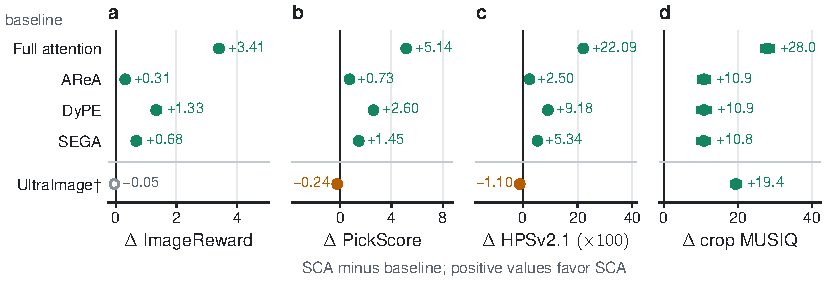
\includegraphics{figures/baseline_deltas.pdf}
  \caption{\textbf{SCA beats every shared-protocol baseline on all four metrics; against UltraImage the result is mixed.}
  SCA minus baseline, mean over the same 191 prompts at $4096^2$, whiskers 95\% prompt-bootstrap intervals (2000 draws, one seed); open markers: interval contains zero; orange: significant loss.
  $^\dagger$Own two-stage recipe, not an equal-cost comparison.}
  \label{fig:baseline_quality}
\end{figure}


\paragraph{$6144^2$ and FLUX.1-Krea-dev.} Table~\ref{tab:krea_6144} gives every metric with its paired interval for the 100-prompt $6144^2$ comparison and for FLUX.1-Krea-dev, where DyPE and SEGA also trail AReA on ImageReward. The Krea table follows the FLUX.1-dev calibration procedure with 16 prompts at $1024^2$ (Appendix~\ref{app:area}).
% Generated by src/gen_late_tables.py from results/e2_6144 and results/e9_krea; do not edit by hand.
\begin{table}[!htbp]
\caption{\textbf{At $6144^2$ \sca{} beats AReA on 14 of 15 metrics; on FLUX.1-Krea-dev it matches AReA in a third of the time.} Method minus AReA with 95\% paired intervals, 100 prompts each; first column FLUX.1-dev at $6144^2$, others FLUX.1-Krea-dev at $4096^2$ with a Krea-calibrated \sca{} table. Per-image intervals use 1000 prompt draws; FID, KID, and their patch versions resample prompts and reference-image clusters. Lower is better for FID, KID, their patch versions, and time. \up{Blue} / \dn{orange}: significantly better / worse than AReA. Time is the campaign mean on shared GH200 nodes.}
\label{tab:krea_6144}
\centering\scriptsize\setlength{\tabcolsep}{2.4pt}\let\tiny\scriptsize
\resizebox{\ifdim\width>\linewidth\linewidth\else\width\fi}{!}{%
\begin{tabular}{lcccc}
\toprule
 & $6144^2$ & \multicolumn{3}{c}{FLUX.1-Krea-dev, $4096^2$} \\
\cmidrule(lr){2-2}\cmidrule(l){3-5}
Metric & \sca{} & \sca{} & DyPE & SEGA \\
\midrule
ImageReward & \up{$+1.262$} {\tiny[$+1.051$, $+1.450$]} & ${-}0.042$ {\tiny[${-}0.118$, $+0.031$]} & \dn{${-}0.282$} {\tiny[${-}0.424$, ${-}0.173$]} & \dn{${-}0.110$} {\tiny[${-}0.189$, ${-}0.030$]} \\
Aesthetic & \up{$+0.44$} {\tiny[$+0.31$, $+0.55$]} & \up{$+0.09$} {\tiny[$+0.04$, $+0.15$]} & $+0.05$ {\tiny[${-}0.02$, $+0.12$]} & ${-}0.05$ {\tiny[${-}0.11$, $+0.02$]} \\
CLIP score & \up{$+3.28$} {\tiny[$+2.32$, $+4.18$]} & ${-}0.08$ {\tiny[${-}0.45$, $+0.27$]} & \dn{${-}0.95$} {\tiny[${-}1.47$, ${-}0.49$]} & \dn{${-}0.49$} {\tiny[${-}0.91$, ${-}0.07$]} \\
PickScore & \up{$+1.58$} {\tiny[$+1.31$, $+1.88$]} & $+0.03$ {\tiny[${-}0.09$, $+0.16$]} & \dn{${-}0.73$} {\tiny[${-}0.93$, ${-}0.55$]} & \dn{${-}0.23$} {\tiny[${-}0.36$, ${-}0.10$]} \\
HPSv2 ($\times100$) & \up{$+2.53$} {\tiny[$+2.12$, $+2.94$]} & \up{$+0.35$} {\tiny[$+0.17$, $+0.53$]} & \dn{${-}1.02$} {\tiny[${-}1.24$, ${-}0.80$]} & \dn{${-}0.25$} {\tiny[${-}0.43$, ${-}0.09$]} \\
HPSv2.1 ($\times100$) & \up{$+6.37$} {\tiny[$+5.39$, $+7.38$]} & \up{$+0.78$} {\tiny[$+0.36$, $+1.17$]} & \dn{${-}1.24$} {\tiny[${-}1.76$, ${-}0.76$]} & ${-}0.25$ {\tiny[${-}0.61$, $+0.09$]} \\
MUSIQ & \up{$+9.2$} {\tiny[$+6.9$, $+11.7$]} & \up{$+1.7$} {\tiny[$+0.3$, $+3.1$]} & \dn{${-}2.6$} {\tiny[${-}4.6$, ${-}0.4$]} & $+0.7$ {\tiny[${-}1.2$, $+2.8$]} \\
MUSIQ$_\text{c}$ & \up{$+3.8$} {\tiny[$+1.4$, $+6.2$]} & \up{$+4.6$} {\tiny[$+3.4$, $+5.7$]} & \up{$+3.2$} {\tiny[$+1.8$, $+4.6$]} & $+1.3$ {\tiny[${-}0.1$, $+2.6$]} \\
CLIP-IQA ($\times100$) & \up{$+6.3$} {\tiny[$+4.3$, $+8.4$]} & $+0.2$ {\tiny[${-}1.2$, $+1.6$]} & $+0.9$ {\tiny[${-}0.7$, $+2.3$]} & \up{$+1.8$} {\tiny[$+0.4$, $+3.2$]} \\
ARNIQA ($\times100$) & \up{$+14.9$} {\tiny[$+13.0$, $+17.0$]} & \up{$+1.5$} {\tiny[$+0.8$, $+2.0$]} & \dn{${-}1.6$} {\tiny[${-}2.6$, ${-}0.7$]} & ${-}0.4$ {\tiny[${-}1.3$, $+0.4$]} \\
\midrule
FID$\downarrow$ & \up{${-}46.8$} {\tiny[${-}58.6$, ${-}35.3$]} & ${-}0.8$ {\tiny[${-}7.9$, $+6.2$]} & $+5.0$ {\tiny[${-}2.8$, $+16.3$]} & ${-}2.3$ {\tiny[${-}10.0$, $+7.4$]} \\
KID$\downarrow$ ($\times10^3$) & \up{${-}23.20$} {\tiny[${-}31.77$, ${-}16.84$]} & $+0.58$ {\tiny[${-}2.02$, $+2.94$]} & ${-}0.81$ {\tiny[${-}4.63$, $+3.26$]} & ${-}0.85$ {\tiny[${-}4.00$, $+1.53$]} \\
FID$_\text{p}\downarrow$ & \up{${-}66.2$} {\tiny[${-}70.2$, ${-}48.9$]} & \dn{$+8.4$} {\tiny[$+4.0$, $+14.2$]} & \dn{$+7.7$} {\tiny[$+5.0$, $+18.5$]} & $+0.1$ {\tiny[${-}3.1$, $+6.7$]} \\
KID$_\text{p}\downarrow$ ($\times10^3$) & \up{${-}56.88$} {\tiny[${-}68.46$, ${-}47.50$]} & $+2.16$ {\tiny[${-}0.20$, $+4.89$]} & $+1.32$ {\tiny[${-}1.44$, $+4.94$]} & ${-}0.81$ {\tiny[${-}2.48$, $+0.90$]} \\
Inception score & $+0.45$ {\tiny[${-}0.06$, $+0.84$]} & ${-}0.11$ {\tiny[${-}0.50$, $+0.33$]} & $+0.25$ {\tiny[${-}0.22$, $+0.69$]} & $+0.09$ {\tiny[${-}0.43$, $+0.56$]} \\
Time (s)$\downarrow$ & \up{${-}343.1$} {\tiny[${-}349.3$, ${-}337.4$]} & \up{${-}144.8$} {\tiny[${-}148.5$, ${-}140.9$]} & \up{${-}24.3$} {\tiny[${-}28.9$, ${-}19.6$]} & \up{${-}20.1$} {\tiny[${-}25.0$, ${-}15.5$]} \\
\bottomrule
\end{tabular}}
\end{table}

\begin{table}[!htbp]
\caption{\textbf{DyPE and SEGA trail \sca{} on every per-image metric; UltraImage and HRDiT are mixed.} Baseline minus \sca{} at $4096^2$, \nmain{} prompts; \up{blue} / \dn{orange}: baseline significantly better / worse than \sca{}. UltraImage and HRDiT use their own multi-stage recipes; HRDiT's set-level metrics are in Table~\ref{tab:main}.}
\label{tab:phase2_baselines}
\centering\scriptsize\setlength{\tabcolsep}{3pt}\let\tiny\scriptsize
\resizebox{\ifdim\width>\linewidth\linewidth\else\width\fi}{!}{%
\begin{tabular}{lcccc}
\toprule
Metric & DyPE & SEGA & UltraImage & HRDiT \\
\midrule
ImageReward & \dn{${-}1.326$} {\tiny[${-}1.466$, ${-}1.185$]} & \dn{${-}0.668$} {\tiny[${-}0.786$, ${-}0.551$]} & $+0.055$ {\tiny[${-}0.011$, $+0.120$]} & \up{$+0.114$} {\tiny[$+0.049$, $+0.181$]} \\
Aesthetic & \dn{${-}0.72$} {\tiny[${-}0.81$, ${-}0.62$]} & \dn{${-}0.42$} {\tiny[${-}0.50$, ${-}0.35$]} & \up{$+0.06$} {\tiny[$+0.01$, $+0.10$]} & \up{$+0.09$} {\tiny[$+0.04$, $+0.13$]} \\
CLIP score & \dn{${-}4.22$} {\tiny[${-}4.85$, ${-}3.62$]} & \dn{${-}2.19$} {\tiny[${-}2.66$, ${-}1.76$]} & \dn{${-}0.31$} {\tiny[${-}0.61$, ${-}0.01$]} & ${-}0.02$ {\tiny[${-}0.32$, $+0.27$]} \\
PickScore & \dn{${-}2.59$} {\tiny[${-}2.78$, ${-}2.40$]} & \dn{${-}1.45$} {\tiny[${-}1.60$, ${-}1.31$]} & \up{$+0.24$} {\tiny[$+0.14$, $+0.33$]} & \up{$+0.37$} {\tiny[$+0.27$, $+0.46$]} \\
HPSv2 ($\times100$) & \dn{${-}4.22$} {\tiny[${-}4.53$, ${-}3.95$]} & \dn{${-}2.61$} {\tiny[${-}2.84$, ${-}2.38$]} & \up{$+0.21$} {\tiny[$+0.06$, $+0.37$]} & $+0.13$ {\tiny[${-}0.02$, $+0.28$]} \\
HPSv2.1 ($\times100$) & \dn{${-}9.12$} {\tiny[${-}9.83$, ${-}8.39$]} & \dn{${-}5.33$} {\tiny[${-}5.84$, ${-}4.78$]} & \up{$+1.10$} {\tiny[$+0.81$, $+1.39$]} & \up{$+1.25$} {\tiny[$+0.97$, $+1.53$]} \\
MUSIQ & \dn{${-}9.1$} {\tiny[${-}11.2$, ${-}7.0$]} & \dn{${-}8.1$} {\tiny[${-}9.9$, ${-}6.3$]} & \dn{${-}11.8$} {\tiny[${-}13.7$, ${-}9.8$]} & \dn{${-}5.1$} {\tiny[${-}6.7$, ${-}3.4$]} \\
MUSIQ$_\text{c}$ & \dn{${-}10.9$} {\tiny[${-}12.8$, ${-}9.2$]} & \dn{${-}11.0$} {\tiny[${-}12.6$, ${-}9.3$]} & \dn{${-}19.5$} {\tiny[${-}20.8$, ${-}18.2$]} & \dn{${-}7.7$} {\tiny[${-}9.0$, ${-}6.4$]} \\
CLIP-IQA ($\times100$) & \dn{${-}13.4$} {\tiny[${-}15.2$, ${-}11.7$]} & \dn{${-}6.3$} {\tiny[${-}8.0$, ${-}4.8$]} & ${-}0.2$ {\tiny[${-}1.2$, $+0.9$]} & \up{$+2.8$} {\tiny[$+1.9$, $+3.8$]} \\
ARNIQA ($\times100$) & \dn{${-}11.1$} {\tiny[${-}12.4$, ${-}9.7$]} & \dn{${-}6.5$} {\tiny[${-}7.6$, ${-}5.4$]} & \up{$+1.0$} {\tiny[$+0.3$, $+1.8$]} & $+0.3$ {\tiny[${-}0.3$, $+0.9$]} \\
\bottomrule
\end{tabular}}
\end{table}
\begin{table}[!htbp]
\caption{\textbf{The gains hold on HRGen-1K, two more seeds, and FLUX.2-dev.} \sca{} minus AReA for HRGen-1K and seeds 1 and 2; \sca{} minus full attention for FLUX.2-dev. All at $4096^2$; \up{blue}: significantly better than the reference.}
\label{tab:phase2_general}
\centering\scriptsize\setlength{\tabcolsep}{2pt}\let\tiny\scriptsize
\resizebox{\ifdim\width>\linewidth\linewidth\else\width\fi}{!}{%
\begin{tabular}{lcccc}
\toprule
Metric & HRGen-1K & Seed 1 & Seed 2 & FLUX.2-dev \\
\midrule
ImageReward & \up{$+0.818$} {\tiny[$+0.768$, $+0.870$]} & \up{$+0.274$} {\tiny[$+0.204$, $+0.349$]} & \up{$+0.250$} {\tiny[$+0.183$, $+0.320$]} & \up{$+0.456$} {\tiny[$+0.320$, $+0.598$]} \\
Aesthetic & \up{$+0.33$} {\tiny[$+0.30$, $+0.36$]} & \up{$+0.14$} {\tiny[$+0.08$, $+0.18$]} & \up{$+0.12$} {\tiny[$+0.06$, $+0.17$]} & \up{$+0.30$} {\tiny[$+0.18$, $+0.42$]} \\
CLIP score & \up{$+2.65$} {\tiny[$+2.40$, $+2.89$]} & \up{$+1.33$} {\tiny[$+1.00$, $+1.63$]} & \up{$+1.45$} {\tiny[$+1.15$, $+1.74$]} & $+0.38$ {\tiny[${-}0.38$, $+1.12$]} \\
PickScore & \up{$+1.19$} {\tiny[$+1.13$, $+1.24$]} & \up{$+0.72$} {\tiny[$+0.60$, $+0.83$]} & \up{$+0.72$} {\tiny[$+0.59$, $+0.84$]} & \up{$+0.56$} {\tiny[$+0.29$, $+0.86$]} \\
HPSv2 ($\times100$) & \up{$+1.95$} {\tiny[$+1.86$, $+2.05$]} & \up{$+1.10$} {\tiny[$+0.94$, $+1.28$]} & \up{$+1.18$} {\tiny[$+0.99$, $+1.37$]} & \up{$+0.85$} {\tiny[$+0.50$, $+1.21$]} \\
HPSv2.1 ($\times100$) & \up{$+4.93$} {\tiny[$+4.70$, $+5.17$]} & \up{$+2.28$} {\tiny[$+1.94$, $+2.62$]} & \up{$+2.50$} {\tiny[$+2.10$, $+2.89$]} & \up{$+1.84$} {\tiny[$+1.10$, $+2.55$]} \\
MUSIQ & \up{$+7.7$} {\tiny[$+6.8$, $+8.5$]} & \up{$+5.6$} {\tiny[$+3.8$, $+7.4$]} & \up{$+5.9$} {\tiny[$+4.0$, $+7.6$]} & \up{$+16.0$} {\tiny[$+11.9$, $+19.9$]} \\
MUSIQ$_\text{c}$ & \up{$+13.9$} {\tiny[$+13.2$, $+14.6$]} & \up{$+11.5$} {\tiny[$+10.2$, $+12.9$]} & \up{$+12.1$} {\tiny[$+10.5$, $+13.6$]} & \up{$+21.4$} {\tiny[$+18.2$, $+24.8$]} \\
CLIP-IQA ($\times100$) & \up{$+9.0$} {\tiny[$+8.3$, $+9.8$]} & \up{$+4.9$} {\tiny[$+3.5$, $+6.3$]} & \up{$+5.0$} {\tiny[$+3.8$, $+6.2$]} & \up{$+6.6$} {\tiny[$+4.7$, $+8.6$]} \\
ARNIQA ($\times100$) & \up{$+7.2$} {\tiny[$+6.7$, $+7.7$]} & \up{$+4.0$} {\tiny[$+3.1$, $+5.0$]} & \up{$+4.0$} {\tiny[$+3.1$, $+4.8$]} & \up{$+7.1$} {\tiny[$+5.4$, $+8.8$]} \\
\bottomrule
\end{tabular}}
\end{table}
\begin{table}[!htbp]
\caption{\textbf{The calibration budget barely matters; a gate at $\sigma_g=0.85$ lowers seven metrics.} Variant minus default \sca{}, \nabl{} ablation prompts; \up{blue} / \dn{orange}: variant significantly better / worse than default \sca{}. Budgets use the first 4, 8, or 16 of the 32 calibration prompts; the default gate is $\sigma_g=0.89$.}
\label{tab:phase2_sensitivity}
\centering\scriptsize\setlength{\tabcolsep}{3pt}
\resizebox{\ifdim\width>\linewidth\linewidth\else\width\fi}{!}{%
\begin{tabular}{l*{5}{Y{57.5pt}}}
\toprule
Metric & 4 prompts & 8 prompts & 16 prompts & $\sigma_g=0.85$ & $\sigma_g=0.93$ \\
\midrule
ImageReward & $+0.012$ {\tiny[${-}0.007$, $+0.029$]} & $+0.010$ {\tiny[${-}0.004$, $+0.024$]} & ${-}0.007$ {\tiny[${-}0.020$, $+0.005$]} & ${-}0.015$ {\tiny[${-}0.098$, $+0.064$]} & ${-}0.004$ {\tiny[${-}0.097$, $+0.069$]} \\
Aesthetic & $+0.01$ {\tiny[${-}0.00$, $+0.02$]} & $+0.01$ {\tiny[${-}0.00$, $+0.02$]} & $+0.00$ {\tiny[${-}0.01$, $+0.01$]} & \dn{${-}0.19$} {\tiny[${-}0.26$, ${-}0.12$]} & $+0.00$ {\tiny[${-}0.05$, $+0.06$]} \\
CLIP score & $+0.08$ {\tiny[${-}0.03$, $+0.19$]} & $+0.05$ {\tiny[${-}0.04$, $+0.15$]} & $+0.04$ {\tiny[${-}0.04$, $+0.13$]} & ${-}0.27$ {\tiny[${-}0.82$, $+0.26$]} & \dn{${-}0.64$} {\tiny[${-}1.03$, ${-}0.29$]} \\
PickScore & ${-}0.01$ {\tiny[${-}0.03$, $+0.01$]} & $+0.00$ {\tiny[${-}0.01$, $+0.02$]} & $+0.01$ {\tiny[${-}0.01$, $+0.03$]} & ${-}0.12$ {\tiny[${-}0.27$, $+0.02$]} & \dn{${-}0.22$} {\tiny[${-}0.38$, ${-}0.07$]} \\
HPSv2 ($\times100$) & $+0.02$ {\tiny[${-}0.02$, $+0.05$]} & $+0.02$ {\tiny[${-}0.00$, $+0.05$]} & $+0.00$ {\tiny[${-}0.02$, $+0.03$]} & \dn{${-}0.48$} {\tiny[${-}0.69$, ${-}0.28$]} & $+0.02$ {\tiny[${-}0.16$, $+0.20$]} \\
HPSv2.1 ($\times100$) & ${-}0.02$ {\tiny[${-}0.07$, $+0.04$]} & $+0.01$ {\tiny[${-}0.03$, $+0.05$]} & ${-}0.01$ {\tiny[${-}0.05$, $+0.04$]} & \dn{${-}0.85$} {\tiny[${-}1.22$, ${-}0.48$]} & ${-}0.15$ {\tiny[${-}0.56$, $+0.24$]} \\
MUSIQ & ${-}0.1$ {\tiny[${-}0.4$, $+0.3$]} & ${-}0.1$ {\tiny[${-}0.5$, $+0.2$]} & \up{$+0.1$} {\tiny[$+0.0$, $+0.3$]} & \dn{${-}1.9$} {\tiny[${-}3.5$, ${-}0.2$]} & $+0.4$ {\tiny[${-}1.0$, $+2.0$]} \\
MUSIQ$_\text{c}$ & $+0.1$ {\tiny[${-}0.1$, $+0.3$]} & ${-}0.0$ {\tiny[${-}0.2$, $+0.1$]} & ${-}0.1$ {\tiny[${-}0.2$, $+0.0$]} & \dn{${-}2.0$} {\tiny[${-}3.0$, ${-}1.1$]} & $+0.6$ {\tiny[${-}0.4$, $+1.9$]} \\
CLIP-IQA ($\times100$) & $+0.2$ {\tiny[${-}0.1$, $+0.4$]} & $+0.2$ {\tiny[${-}0.1$, $+0.4$]} & ${-}0.1$ {\tiny[${-}0.4$, $+0.1$]} & \dn{${-}3.2$} {\tiny[${-}4.8$, ${-}1.7$]} & $+0.0$ {\tiny[${-}1.2$, $+1.1$]} \\
ARNIQA ($\times100$) & $+0.1$ {\tiny[${-}0.1$, $+0.3$]} & $+0.0$ {\tiny[${-}0.1$, $+0.2$]} & ${-}0.0$ {\tiny[${-}0.1$, $+0.1$]} & \dn{${-}4.0$} {\tiny[${-}5.9$, ${-}2.3$]} & \up{$+1.8$} {\tiny[$+0.7$, $+3.1$]} \\
\bottomrule
\end{tabular}}
\end{table}
\begin{table}[!htbp]
\caption{\textbf{All three added baselines have significantly higher FID, patch FID, and patch KID than \sca{}.} Method minus \sca{} on \nmain{} prompts (negative favours the method); \dn{orange}: significantly worse than \sca{}. Patch estimates use corrected crops; all four intervals use 1000 draws that resample generated prompts and reference-image clusters.}
\label{tab:phase2_distribution}
\centering\scriptsize\setlength{\tabcolsep}{3pt}\let\tiny\scriptsize
\resizebox{\ifdim\width>\linewidth\linewidth\else\width\fi}{!}{%
\begin{tabular}{lccc}
\toprule
Metric & DyPE & SEGA & UltraImage \\
\midrule
FID$\downarrow$ & \dn{$+67.4$} {\tiny[$+56.2$, $+80.3$]} & \dn{$+26.9$} {\tiny[$+21.1$, $+39.1$]} & \dn{$+4.0$} {\tiny[$+1.1$, $+10.2$]} \\
KID$\downarrow$ ($\times10^3$) & \dn{$+40.39$} {\tiny[$+30.63$, $+52.87$]} & \dn{$+4.70$} {\tiny[$+0.14$, $+10.48$]} & $+0.19$ {\tiny[${-}1.83$, $+2.18$]} \\
FID$_\text{p}\downarrow$ & \dn{$+72.8$} {\tiny[$+58.7$, $+81.6$]} & \dn{$+26.7$} {\tiny[$+18.8$, $+35.3$]} & \dn{$+10.4$} {\tiny[$+6.2$, $+13.9$]} \\
KID$_\text{p}\downarrow$ ($\times10^3$) & \dn{$+49.34$} {\tiny[$+40.09$, $+59.95$]} & \dn{$+13.97$} {\tiny[$+9.33$, $+20.00$]} & \dn{$+7.31$} {\tiny[$+5.10$, $+9.47$]} \\
\bottomrule
\end{tabular}}
\end{table}

\paragraph{\npanel-prompt panel.} Table~\ref{tab:panel46_deltas} pairs each baseline of Table~\ref{tab:panel46} with \sca{} on the same \npanel{} prompts and seeds. Per-image intervals use 2000 prompt draws with seed 0; FID, KID, and their patch versions use 1000 draws that resample generated prompts and reference-image clusters. \ifpanelfull{}{With \npanel{} generated images, the whole-image distribution metrics are exploratory.} Table~\ref{tab:phase2_budget} gives the matching intervals for the 56-step and guidance-7 \sca{} runs.
\begin{table}[!htbp]
\caption{\textbf{On the \npanel-prompt panel, every shared-protocol baseline trails \sca{} on all ten per-image metrics, while HRDiT and UltraImage lead on several preference metrics.} Baseline minus \sca{} (28 steps) at $4096^2$ with 95\% paired intervals; HPSv2, HPSv2.1, CLIP-IQA, and ARNIQA are $\times100$, KID and KID$_\text{p}$ $\times10^3$. For FID, KID, their patch versions, and campaign time (seconds per image), lower is better, so negative favours the baseline. \up{Blue} / \dn{orange}: baseline significantly better / worse than \sca{}. SigMa uses its dev-matched profile; UltraImage and HRDiT use their own recipes (Appendix~\ref{app:additional_protocols}).}
\label{tab:panel46_deltas}
\centering\scriptsize\setlength{\tabcolsep}{2.5pt}\let\tiny\scriptsize
\begin{tabular}{l*{5}{Y{62pt}}}
\toprule
 & \multicolumn{5}{c}{\emph{Single pass, shared sampler}} \\
\cmidrule(l){2-6}
Metric & Full attn. & DyPE & SigMa & SEGA & AReA \\
\midrule
ImageReward & \dn{${-}3.409$} {\tiny[${-}3.509$, ${-}3.308$]} & \dn{${-}1.326$} {\tiny[${-}1.466$, ${-}1.185$]} & \dn{${-}1.751$} {\tiny[${-}1.898$, ${-}1.605$]} & \dn{${-}0.668$} {\tiny[${-}0.786$, ${-}0.551$]} & \dn{${-}0.308$} {\tiny[${-}0.381$, ${-}0.234$]} \\
Aesthetic & \dn{${-}1.94$} {\tiny[${-}2.03$, ${-}1.85$]} & \dn{${-}0.72$} {\tiny[${-}0.81$, ${-}0.62$]} & \dn{${-}0.84$} {\tiny[${-}0.94$, ${-}0.75$]} & \dn{${-}0.42$} {\tiny[${-}0.50$, ${-}0.35$]} & \dn{${-}0.17$} {\tiny[${-}0.22$, ${-}0.12$]} \\
CLIP score & \dn{${-}13.77$} {\tiny[${-}14.59$, ${-}12.98$]} & \dn{${-}4.22$} {\tiny[${-}4.85$, ${-}3.62$]} & \dn{${-}5.63$} {\tiny[${-}6.31$, ${-}4.95$]} & \dn{${-}2.19$} {\tiny[${-}2.66$, ${-}1.76$]} & \dn{${-}1.45$} {\tiny[${-}1.81$, ${-}1.11$]} \\
PickScore & \dn{${-}5.15$} {\tiny[${-}5.37$, ${-}4.96$]} & \dn{${-}2.59$} {\tiny[${-}2.78$, ${-}2.40$]} & \dn{${-}3.08$} {\tiny[${-}3.29$, ${-}2.87$]} & \dn{${-}1.45$} {\tiny[${-}1.60$, ${-}1.31$]} & \dn{${-}0.74$} {\tiny[${-}0.86$, ${-}0.63$]} \\
HPSv2 & \dn{${-}9.00$} {\tiny[${-}9.33$, ${-}8.66$]} & \dn{${-}4.22$} {\tiny[${-}4.53$, ${-}3.95$]} & \dn{${-}4.97$} {\tiny[${-}5.29$, ${-}4.69$]} & \dn{${-}2.61$} {\tiny[${-}2.84$, ${-}2.38$]} & \dn{${-}1.13$} {\tiny[${-}1.31$, ${-}0.95$]} \\
HPSv2.1 & \dn{${-}22.07$} {\tiny[${-}22.89$, ${-}21.27$]} & \dn{${-}9.12$} {\tiny[${-}9.83$, ${-}8.39$]} & \dn{${-}11.02$} {\tiny[${-}11.78$, ${-}10.29$]} & \dn{${-}5.33$} {\tiny[${-}5.84$, ${-}4.78$]} & \dn{${-}2.51$} {\tiny[${-}2.87$, ${-}2.13$]} \\
MUSIQ & \dn{${-}22.5$} {\tiny[${-}24.2$, ${-}20.8$]} & \dn{${-}9.1$} {\tiny[${-}11.2$, ${-}7.0$]} & \dn{${-}9.9$} {\tiny[${-}12.0$, ${-}7.8$]} & \dn{${-}8.1$} {\tiny[${-}9.9$, ${-}6.3$]} & \dn{${-}6.0$} {\tiny[${-}7.8$, ${-}4.4$]} \\
MUSIQ$_\text{c}$ & \dn{${-}28.1$} {\tiny[${-}29.8$, ${-}26.5$]} & \dn{${-}10.9$} {\tiny[${-}12.8$, ${-}9.2$]} & \dn{${-}11.4$} {\tiny[${-}13.2$, ${-}9.6$]} & \dn{${-}11.0$} {\tiny[${-}12.6$, ${-}9.3$]} & \dn{${-}10.8$} {\tiny[${-}12.3$, ${-}9.4$]} \\
CLIP-IQA & \dn{${-}24.0$} {\tiny[${-}25.5$, ${-}22.5$]} & \dn{${-}13.4$} {\tiny[${-}15.2$, ${-}11.7$]} & \dn{${-}15.0$} {\tiny[${-}16.9$, ${-}13.1$]} & \dn{${-}6.3$} {\tiny[${-}8.0$, ${-}4.8$]} & \dn{${-}5.3$} {\tiny[${-}6.7$, ${-}3.9$]} \\
ARNIQA & \dn{${-}16.8$} {\tiny[${-}18.3$, ${-}15.4$]} & \dn{${-}11.1$} {\tiny[${-}12.4$, ${-}9.7$]} & \dn{${-}11.4$} {\tiny[${-}12.8$, ${-}10.0$]} & \dn{${-}6.5$} {\tiny[${-}7.6$, ${-}5.4$]} & \dn{${-}3.9$} {\tiny[${-}4.9$, ${-}3.0$]} \\
FID$\downarrow$ & \dn{$+174.4$} {\tiny[$+150.2$, $+179.4$]} & \dn{$+67.4$} {\tiny[$+56.2$, $+80.3$]} & \dn{$+78.9$} {\tiny[$+66.7$, $+91.0$]} & \dn{$+26.9$} {\tiny[$+21.1$, $+39.1$]} & \dn{$+7.7$} {\tiny[$+2.6$, $+13.1$]} \\
KID$\downarrow$ & \dn{$+158.0$} {\tiny[$+140.3$, $+176.0$]} & \dn{$+40.4$} {\tiny[$+30.6$, $+52.9$]} & \dn{$+50.4$} {\tiny[$+39.1$, $+64.0$]} & \dn{$+4.7$} {\tiny[$+0.1$, $+10.5$]} & $+1.0$ {\tiny[${-}1.5$, $+3.2$]} \\
FID$_\text{p}\downarrow$ & \dn{$+153.1$} {\tiny[$+122.3$, $+149.6$]} & \dn{$+72.8$} {\tiny[$+58.7$, $+81.6$]} & \dn{$+85.5$} {\tiny[$+70.2$, $+93.7$]} & \dn{$+26.7$} {\tiny[$+18.8$, $+35.3$]} & $+3.8$ {\tiny[${-}1.3$, $+7.5$]} \\
KID$_\text{p}\downarrow$ & \dn{$+161.9$} {\tiny[$+146.6$, $+178.2$]} & \dn{$+49.3$} {\tiny[$+40.1$, $+60.0$]} & \dn{$+62.4$} {\tiny[$+52.0$, $+74.7$]} & \dn{$+14.0$} {\tiny[$+9.3$, $+20.0$]} & $+2.3$ {\tiny[${-}0.1$, $+4.6$]} \\
Time (s)$\downarrow$ & \dn{$+124.7$} {\tiny[$+120.8$, $+129.4$]} & \dn{$+124.4$} {\tiny[$+120.5$, $+128.6$]} & \dn{$+121.0$} {\tiny[$+119.0$, $+123.0$]} & \dn{$+118.9$} {\tiny[$+118.0$, $+119.7$]} & \dn{$+192.9$} {\tiny[$+180.3$, $+206.4$]} \\
\bottomrule
\end{tabular}

\medskip
\begin{tabular}{lcc}
\toprule
 & \multicolumn{2}{c}{\emph{Multi-stage, own recipe}} \\
\cmidrule(l){2-3}
Metric & UltraImage & HRDiT \\
\midrule
ImageReward & $+0.055$ {\tiny[${-}0.011$, $+0.120$]} & \up{$+0.114$} {\tiny[$+0.049$, $+0.181$]} \\
Aesthetic & \up{$+0.06$} {\tiny[$+0.01$, $+0.10$]} & \up{$+0.09$} {\tiny[$+0.04$, $+0.13$]} \\
CLIP score & \dn{${-}0.31$} {\tiny[${-}0.61$, ${-}0.01$]} & ${-}0.02$ {\tiny[${-}0.32$, $+0.27$]} \\
PickScore & \up{$+0.24$} {\tiny[$+0.14$, $+0.33$]} & \up{$+0.37$} {\tiny[$+0.27$, $+0.46$]} \\
HPSv2 & \up{$+0.21$} {\tiny[$+0.06$, $+0.37$]} & $+0.13$ {\tiny[${-}0.02$, $+0.28$]} \\
HPSv2.1 & \up{$+1.10$} {\tiny[$+0.81$, $+1.39$]} & \up{$+1.25$} {\tiny[$+0.97$, $+1.53$]} \\
MUSIQ & \dn{${-}11.8$} {\tiny[${-}13.7$, ${-}9.8$]} & \dn{${-}5.1$} {\tiny[${-}6.7$, ${-}3.4$]} \\
MUSIQ$_\text{c}$ & \dn{${-}19.5$} {\tiny[${-}20.8$, ${-}18.2$]} & \dn{${-}7.7$} {\tiny[${-}9.0$, ${-}6.4$]} \\
CLIP-IQA & ${-}0.2$ {\tiny[${-}1.2$, $+0.9$]} & \up{$+2.8$} {\tiny[$+1.9$, $+3.8$]} \\
ARNIQA & \up{$+1.0$} {\tiny[$+0.3$, $+1.8$]} & $+0.3$ {\tiny[${-}0.3$, $+0.9$]} \\
FID$\downarrow$ & \dn{$+4.0$} {\tiny[$+1.1$, $+10.2$]} & $+0.4$ {\tiny[${-}2.3$, $+6.4$]} \\
KID$\downarrow$ & $+0.2$ {\tiny[${-}1.8$, $+2.2$]} & ${-}1.6$ {\tiny[${-}3.6$, $+0.3$]} \\
FID$_\text{p}\downarrow$ & \dn{$+10.4$} {\tiny[$+6.2$, $+13.9$]} & \dn{$+3.9$} {\tiny[$+0.7$, $+8.0$]} \\
KID$_\text{p}\downarrow$ & \dn{$+7.3$} {\tiny[$+5.1$, $+9.5$]} & \dn{$+2.8$} {\tiny[$+0.9$, $+4.8$]} \\
Time (s)$\downarrow$ & \dn{$+237.0$} {\tiny[$+233.5$, $+241.7$]} & \dn{$+38.8$} {\tiny[$+37.2$, $+40.5$]} \\
\bottomrule
\end{tabular}
\end{table}

\FloatBarrier
\section{Sampling-budget, guidance, and schedule checks}
\label{app:budget}

This section expands the budget and schedule rows of Table~\ref{tab:panel46}: Figure~\ref{fig:quality_time} plots quality against time, Table~\ref{tab:phase2_budget} gives the budget and guidance checks, Table~\ref{tab:prog_deltas} the progressive schedule against HRDiT, and Figure~\ref{fig:progressive} two random prompts under each schedule.

\begin{figure}[!htbp]
  \centering
  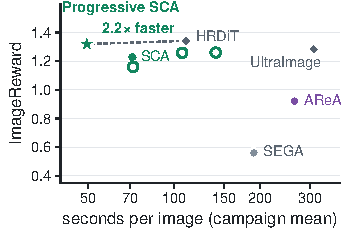
\includegraphics[width=0.5\linewidth]{figures/quality_time_wrap.pdf}
  \caption{\textbf{Quality against time.} \npanel{} prompts, $4096^2$. Open circles: \sca{} at guidance 7, 42 and 56 steps.}
  \label{fig:quality_time}
\end{figure}

On the same \npanel{} evaluation prompts, we compare the default 28-step \sca{} run with 56 steps at guidance 4.5 and with 28 steps at guidance 7 (Table~\ref{tab:phase2_budget}). The 56-step run keeps the noise threshold at 0.89; it therefore changes the discretization of both the opening and mixed phases. It improves ImageReward by 0.032 $[0.0002,0.062]$, HPSv2.1 by 0.88, PickScore by 0.13, and MUSIQ$_\text{c}$ by 2.90, but increases corrected patch FID by 3.85 $[1.51,6.33]$ with reference-image cluster resampling. Increasing guidance to 7 alone lowers seven per-image metrics, ImageReward by 0.068 $[0.025,0.115]$ among them, and raises only MUSIQ. Thus the default schedule does not maximize every metric, and extra sampling can change the preference-quality balance.

Against UltraImage on these \npanel{} prompts, 56-step \sca{} has ImageReward difference $-0.023$ $[-0.089,0.040]$, HPSv2.1 difference $-0.22$ $[-0.51,0.05]$, and PickScore difference $-0.11$ $[-0.21,-0.01]$. The first two intervals span zero and do not establish equivalence; PickScore favours UltraImage. Its MUSIQ advantage is 11.61 $[9.54,13.60]$ and its MUSIQ$_\text{c}$ advantage 22.42 $[21.20,23.59]$. Campaign means are 71.5\,s for default \sca{}, 139.9\,s for 56-step \sca{}, and 308.5\,s for UltraImage on these \npanel{} prompts. This is a sampling-budget sensitivity check, not an equal-FLOP or equal-wall-clock experiment: UltraImage has two resolutions, different guidance, and per-prompt preparation. Against HRDiT on the same prompts (Table~\ref{tab:panel46}), the 56-step run stays lower on ImageReward (1.26 against 1.34), HPSv2.1 (30.55 against 30.92), and PickScore (23.22 against 23.46) while taking longer (139.9 against 110.4\,s); these are point estimates without paired intervals. Table~\ref{tab:prog_deltas} adds a 42-step run sized to HRDiT's campaign time (106.8 against 110.4\,s) and progressive \sca{} (Section~\ref{sec:progressive}). The extra steps raise PickScore, HPSv2, HPSv2.1, ARNIQA, and MUSIQ$_\text{c}$ over 28 steps but leave ImageReward unresolved, and HRDiT stays significantly ahead of the 42-step run on ImageReward, PickScore, HPSv2.1, aesthetic score, and CLIP-IQA while trailing it on both MUSIQ scores and ARNIQA. Progressive \sca{} is significantly worse than HRDiT on no per-image metric and better on HPSv2, MUSIQ, and ARNIQA; against single-pass \sca{} it gains ImageReward, PickScore, aesthetic score, both HPS scores, CLIP-IQA, and ARNIQA, and loses both MUSIQ scores. Figure~\ref{fig:quality_time} places every setting of the panel by ImageReward and time, and Figure~\ref{fig:progressive} shows HRDiT, progressive \sca{}, and single-pass \sca{} on two random prompts.

\begin{table}[!htbp]
\caption{\textbf{Doubling the steps raises eight metrics; guidance 7 lowers seven and raises MUSIQ.} On \npanel{} prompts, the first two columns compare with default \sca{}; the last compares 56-step \sca{} with UltraImage. Per-image differences (first-named setting minus second) and 95\% paired intervals, 2000 draws; \up{blue} / \dn{orange}: the interval excludes zero in favour of / against the first-named setting.}
\label{tab:phase2_budget}
\centering\scriptsize\setlength{\tabcolsep}{3pt}\let\tiny\scriptsize
\resizebox{\ifdim\width>\linewidth\linewidth\else\width\fi}{!}{%
\begin{tabular}{lccc}
\toprule
Metric & 56 vs.\ 28 steps & Guidance 7 vs.\ 4.5 & 56 steps vs.\ UltraImage \\
\midrule
ImageReward & \up{$+0.032$} {\tiny[$+0.000$, $+0.062$]} & \dn{${-}0.068$} {\tiny[${-}0.115$, ${-}0.025$]} & ${-}0.023$ {\tiny[${-}0.089$, $+0.040$]} \\
Aesthetic & \up{$+0.03$} {\tiny[$+0.01$, $+0.06$]} & \dn{${-}0.10$} {\tiny[${-}0.14$, ${-}0.07$]} & ${-}0.03$ {\tiny[${-}0.07$, $+0.02$]} \\
CLIP score & ${-}0.01$ {\tiny[${-}0.23$, $+0.22$]} & ${-}0.21$ {\tiny[${-}0.45$, $+0.03$]} & $+0.30$ {\tiny[${-}0.01$, $+0.62$]} \\
PickScore & \up{$+0.13$} {\tiny[$+0.07$, $+0.18$]} & \dn{${-}0.27$} {\tiny[${-}0.34$, ${-}0.20$]} & \dn{${-}0.11$} {\tiny[${-}0.21$, ${-}0.01$]} \\
HPSv2 ($\times100$) & \up{$+0.32$} {\tiny[$+0.23$, $+0.40$]} & \dn{${-}0.25$} {\tiny[${-}0.35$, ${-}0.16$]} & $+0.11$ {\tiny[${-}0.03$, $+0.26$]} \\
HPSv2.1 ($\times100$) & \up{$+0.88$} {\tiny[$+0.71$, $+1.04$]} & \dn{${-}0.60$} {\tiny[${-}0.80$, ${-}0.41$]} & ${-}0.22$ {\tiny[${-}0.51$, $+0.05$]} \\
MUSIQ & ${-}0.2$ {\tiny[${-}1.5$, $+1.0$]} & \up{$+1.4$} {\tiny[$+0.3$, $+2.6$]} & \up{$+11.6$} {\tiny[$+9.5$, $+13.6$]} \\
MUSIQ$_\text{c}$ & \up{$+2.9$} {\tiny[$+2.2$, $+3.6$]} & $+0.2$ {\tiny[${-}0.4$, $+0.8$]} & \up{$+22.4$} {\tiny[$+21.2$, $+23.6$]} \\
CLIP-IQA ($\times100$) & \up{$+0.9$} {\tiny[$+0.4$, $+1.4$]} & \dn{${-}1.0$} {\tiny[${-}1.7$, ${-}0.4$]} & \up{$+1.1$} {\tiny[$+0.0$, $+2.1$]} \\
ARNIQA ($\times100$) & \up{$+1.5$} {\tiny[$+1.0$, $+1.9$]} & \dn{${-}1.2$} {\tiny[${-}1.5$, ${-}0.8$]} & $+0.4$ {\tiny[${-}0.4$, $+1.2$]} \\
\bottomrule
\end{tabular}}
\end{table}

\paragraph{Distribution metrics of the progressive and 42-step runs.} Against single-pass \sca{} at 28 steps (\npanel{} generated images, 168 reference identities, 1000 bootstrap draws; \texttt{results/\allowbreak a4k195\_panel/\allowbreak corrected\_fidp\_ci/\allowbreak paired\_deltas.csv}), progressive \sca{} has significantly higher patch FID ($+7.2$ $[3.2,11.0]$) and patch KID ($+0.005$ $[0.003,0.007]$), while its FID ($+3.0$ $[-0.2,8.3]$) and KID differences span zero. For 42-step \sca{} only FID is significantly higher ($+2.4$ $[0.1,5.7]$); KID, patch FID ($+1.5$ $[-0.5,3.6]$), and patch KID span zero.

% Generated by src/gen_prog_tables.py from results/progressive46; do not edit by hand.
\begin{table}[!htbp]
\caption{\textbf{Against HRDiT, progressive \sca{} is not significantly worse on any per-image metric; single-pass \sca{} with 42 steps is.} $4096^2$, 46 prompts, seed label 0. Per-image differences (first-named setting minus second) with 95\% paired intervals over 2000 prompt draws; \up{blue} / \dn{orange}: the interval excludes zero in favour of / against the first-named setting. Progressive: HRDiT's schedule with \sca{} attention (Section~\ref{sec:progressive}); 42 steps: single-pass \sca{} sized to HRDiT's campaign time. Intervals that include zero do not establish equivalence.}
\label{tab:prog_deltas}
\centering\scriptsize\setlength{\tabcolsep}{2.4pt}\let\tiny\scriptsize
\resizebox{\ifdim\width>\linewidth\linewidth\else\width\fi}{!}{%
\begin{tabular}{lcccc}
\toprule
Metric & Progressive vs.\ HRDiT & Progressive vs.\ \sca{} & 42 steps vs.\ \sca{} & HRDiT vs.\ 42 steps \\
\midrule
ImageReward & ${-}0.077$ {\tiny[${-}0.197$, $+0.030$]} & \up{$+0.172$} {\tiny[$+0.019$, $+0.305$]} & $+0.062$ {\tiny[${-}0.003$, $+0.123$]} & \up{$+0.187$} {\tiny[$+0.073$, $+0.314$]} \\
Aesthetic & ${-}0.051$ {\tiny[${-}0.129$, $+0.027$]} & $+0.073$ {\tiny[${-}0.003$, $+0.155$]} & $+0.029$ {\tiny[${-}0.029$, $+0.082$]} & \up{$+0.095$} {\tiny[$+0.003$, $+0.187$]} \\
CLIP score & ${-}0.36$ {\tiny[${-}0.83$, $+0.11$]} & ${-}0.39$ {\tiny[${-}0.91$, $+0.11$]} & ${-}0.29$ {\tiny[${-}0.81$, $+0.15$]} & $+0.26$ {\tiny[${-}0.40$, $+0.96$]} \\
PickScore & ${-}0.02$ {\tiny[${-}0.18$, $+0.14$]} & \up{$+0.44$} {\tiny[$+0.27$, $+0.62$]} & $+0.06$ {\tiny[${-}0.06$, $+0.19$]} & \up{$+0.40$} {\tiny[$+0.19$, $+0.63$]} \\
HPSv2 ($\times100$) & \up{$+0.46$} {\tiny[$+0.20$, $+0.74$]} & \up{$+0.73$} {\tiny[$+0.41$, $+1.06$]} & \up{$+0.20$} {\tiny[$+0.01$, $+0.39$]} & $+0.07$ {\tiny[${-}0.32$, $+0.48$]} \\
HPSv2.1 ($\times100$) & $+0.28$ {\tiny[${-}0.21$, $+0.77$]} & \up{$+1.90$} {\tiny[$+1.18$, $+2.61$]} & \up{$+0.64$} {\tiny[$+0.28$, $+1.06$]} & \up{$+0.98$} {\tiny[$+0.29$, $+1.70$]} \\
MUSIQ & $+1.6$ {\tiny[${-}0.5$, $+3.7$]} & ${-}3.5$ {\tiny[${-}7.0$, $+0.4$]} & ${-}0.4$ {\tiny[${-}2.2$, $+1.2$]} & \dn{${-}4.7$} {\tiny[${-}8.1$, ${-}1.2$]} \\
MUSIQ$_\text{c}$ & $+0.7$ {\tiny[${-}2.3$, $+3.8$]} & \dn{${-}7.7$} {\tiny[${-}11.1$, ${-}4.5$]} & \up{$+1.5$} {\tiny[$+0.3$, $+2.6$]} & \dn{${-}9.9$} {\tiny[${-}13.1$, ${-}6.7$]} \\
CLIP-IQA ($\times100$) & ${-}0.1$ {\tiny[${-}1.7$, $+1.4$]} & \up{$+2.7$} {\tiny[$+0.6$, $+4.7$]} & $+0.5$ {\tiny[${-}0.6$, $+1.5$]} & \up{$+2.3$} {\tiny[$+0.5$, $+4.1$]} \\
ARNIQA ($\times100$) & \up{$+3.0$} {\tiny[$+2.0$, $+4.0$]} & \up{$+4.0$} {\tiny[$+2.5$, $+5.6$]} & \up{$+1.2$} {\tiny[$+0.4$, $+2.0$]} & ${-}0.2$ {\tiny[${-}1.6$, $+1.3$]} \\
\bottomrule
\end{tabular}}
\end{table}

% Generated by src/fig_progressive.py (TikZ source src/progressive.tex, assets figures/progressive/cmp_*).
\begin{figure}[t]
  \centering
  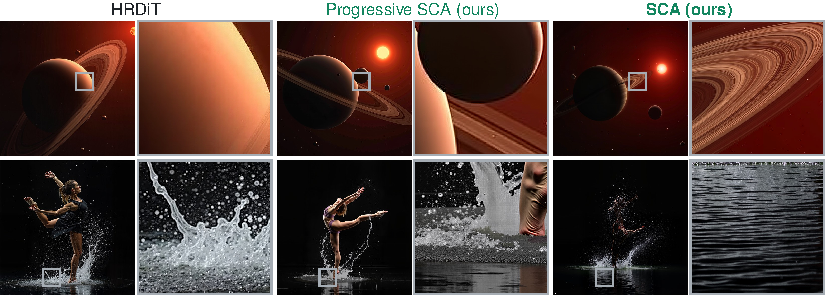
\includegraphics[width=\linewidth]{figures/progressive.pdf}
  \caption{\textbf{Progressive \sca{} (HRDiT's schedule, \sca{} attention) keeps one large subject as HRDiT does, while single-pass \sca{} can shrink or repeat subjects in these prompts.} Seed~0; two prompts drawn at random (seed~17) from the 46-prompt panel; crops are the same native ${512\times512}$ window per row, auto-placed at maximal edge energy averaged over the three methods. Times are 46-prompt campaign means (Table~\ref{tab:panel46}, Section~\ref{sec:progressive}).}
  \label{fig:progressive}
\end{figure}


\FloatBarrier
\section{Exploratory \texorpdfstring{$8192^2$}{8192x8192} comparison}
\label{app:8k}

Table~\ref{tab:e2_8192_per_image} reports all 12 completed prompt pairs at $8192^2$ under the shared FLUX.1-dev protocol. \sca{} has higher ImageReward, CLIP, PickScore, both HPS variants, and ARNIQA, with paired intervals excluding zero. Aesthetic score and the three remaining quality metrics have intervals spanning zero. In particular, MUSIQ, MUSIQ$_\text{c}$, and CLIP-IQA have point estimates favouring AReA. These mixed quality scores and the grid and stripe failures in Figure~\ref{fig:gallery_8192_complete} limit the evidence for reliable 8K generation. With only 12 prompts, this comparison is exploratory; we do not report distributional metrics for this set.

All 8K scores were computed on CPU. HPS uses float32 here, whereas the main GPU evaluation uses mixed precision, so absolute scores across resolutions should not be interpreted as a controlled scaling comparison. Both methods within this table use the same evaluator settings. For native-resolution MUSIQ, attention queries are processed in chunks of 256 while retaining every key and native image patch. This bounds intermediate memory without changing the attention context; pretrained equivalence checks at three smaller image sizes reproduced the unchunked scores exactly.

\snippet{e2_8192_tables}{}

\FloatBarrier
\section{Calibration table at non-square sizes}
\label{app:ps2}

At $(s_H,s_W)=(2,4)$ the two axes have different factors, and \sca{} uses the table of the emulated scale nearest the larger factor, scale 4. On the \nabl{} ablation prompts at $2048\times4096$, the scale-2 table changes the paired metrics negligibly (Table~\ref{tab:app_ps2}): HPSv2 $+0.09$, HPSv2.1 $+0.17$ (both $\times100$), and PickScore $+0.05$ are significant but small, and ImageReward ($+0.01$ $[-0.03,0.05]$) and the other metrics are within noise. These small changes do not resolve the mixed \sca{}--AReA results at this size, and we keep the default rule.

\FloatBarrier
\section{Late duplication: detector and variants}
\label{app:dupfix}
This section expands Sections~\ref{sec:rootcause} and~\ref{sec:dup} and Figure~\ref{fig:dup}: how duplicates are counted, how well the count agrees with visual review, and every variant of the schedule we ran on the 46-prompt subset.

\paragraph{Detector.} Grounding DINO~\citep{liu2023groundingdino} (the released tiny checkpoint) runs on each image at two scales, longest side 800 and 1333 pixels, with all subjects of the prompt joined into one text query; a box counts when its score is at least 0.35, the detector's default, fixed before any image was scored. Boxes from both scales are merged by non-maximum suppression at IoU 0.5 and by containment (at least 90\% of a box inside another of at least 30\% of its area), and boxes covering over 90\% of the image are dropped. Subject lists and implied counts were written from the prompt text alone, before any image was scored. A prompt is eligible when it implies a count for a person or an animal: 95 of the 195 Aesthetic-4K prompts and 26 of the 46-prompt subset. An image is duplicated when any such count exceeds the implied count. Rates carry Wilson 95\% intervals, and paired comparisons use an exact McNemar test.

\paragraph{Validation.} We compared the detector with visual labels of 30 images of \sca{} without the schedule. On the 20 images whose prompt names a person or an animal, it agrees with the original labels on 18; inspecting the two disagreements at full resolution showed small copies the first review had missed (three climbers along the top edge of the ice-climber image, a second portrait of the man in the artist's corner), so it agrees with the reviewed labels on all 20. Over any counted subject it agrees on 26 of 30, with two false positives (a brimmed hat read as a second umbrella, a two-channel waterfall) and two misses. Thresholds from 0.3 to 0.4 give the same rates.

\paragraph{Variants.} Table~\ref{tab:dupfix} lists every variant we ran on the 46 prompts, with its duplication count, time per image, and the per-image metrics on which it is significantly worse than \sca{} without the schedule. Losses are split between prompts whose duplicates the variant removes and prompts clean under both operators; a loss on the clean prompts is real softening. Every variant that alters the whole trajectory (a held low band, wide windows with the scale-4 weight, a larger bridge) softens clean prompts. The bridge alone is nearly free but leaves 5 of 26 prompts duplicated. The schedule with ratio-matched weights is the best trade-off we found.
\snippet{dupfix_variants}{}

\paragraph{Examples.} The pairs in Figure~\ref{fig:dup}c follow a rule fixed before any image of the final operator was viewed.\snippet{dup_examples_rule}{}

\FloatBarrier
\section{The low-band duplication guard}
\label{app:band}
The band guard was our first fix for late duplication. It acts on the operator without the schedule and is not part of \sca{}; the window schedule of Section~\ref{sec:sched} replaced it (Appendix~\ref{app:dupfix}).

\paragraph{Construction.} Let $\LP$ average-pool a head's image output over $p\times p$ tokens and upsample it bilinearly, and $\HP=\mathrm{I}-\LP$. The guard replaces the low band of the mix $M$ by that of the global branch:
\begin{equation}
  O \;=\; \LP\big(\Oglob\big) + \HP\big(M\big) \;=\; \Oglob + \pih\,\HP\big(\Oloc-\Oglob\big).
\end{equation}
The local branch then contributes only its difference from the global branch above the cutoff. The cutoff should lie below $1/(2s)$, where the global branch aliases, and above $1/w$, below which the window cannot resolve; with $w=64$ and $s=4$ this leaves periods of 8 to 64 tokens. We used $p=16$; $p=8$ and $p=32$ were worse on four development prompts, and a noise-dependent cutoff behaved like $p=16$. FreeScale~\citep{qiu2024freescale} also fuses two self-attention outputs by frequency band, in the opposite direction: it keeps the blurred low band of attention over overlapping crops and takes the high band from full self-attention at the target size. ResDiT also combines global low frequencies and local high frequencies, using patch-wise FFT masks~\citep{ma2025resdit}. Our optional guard uses pooled global attention and preserves the fitted per-head weight on the local-minus-global high-band residual. Its global-low/local-high construction is therefore not itself novel.

\begin{table}[!htbp]
  \caption{\textbf{Ablations around the band-guard configuration at $4096^2$}, \nabl{} ablation prompts. The reference row gives absolute values for \sca{} + band guard (band 16); every other row changes one thing, keeps the guard unless stated, and reports its paired difference to the reference. Marks and units as in Table~\ref{tab:ablation}; corrected patch FID is shown without intervals.}
  \label{tab:ablation_band}
  \centering
  \scriptsize
  \setlength{\tabcolsep}{1.6pt}
  \resizebox{\linewidth}{!}{%
  \begin{tabular}{lcccccccccccc}
    \toprule
    Variant & Mix err. & \begin{tabular}[b]{@{}c@{}}Image\\Reward\end{tabular} & Aesth. & HPSv2 & HPSv2.1 & \begin{tabular}[b]{@{}c@{}}Pick\\Score\end{tabular} & CLIP & CLIP-IQA & ARNIQA & MUSIQ & MUSIQ$_\text{c}$ & FID$_\text{p}\downarrow$ \\
    \midrule
    \sca{} + band guard (reference) & 0.200 & 1.17 & 6.43 & 29.18 & 28.81 & 22.71 & 29.01 & 69.6 & 69.6 & 43.1 & 62.1 & 166.7 \\
    \midrule
    no band (\textbf{= \sca{} final}) & 0.200 & $-0.04$ & $+0.01$ & \up{$+0.54$} & \up{$+1.17$} & \up{$+0.25$} & $+0.40$ & \up{$+1.7$} & $+0.9$ & \up{$+2.9$} & $+0.4$ & $+1.3$ \\
    no gate & 0.200 & \dn{$-0.36$} & \dn{$-0.23$} & \dn{$-0.49$} & \dn{$-1.39$} & \dn{$-0.86$} & \dn{$-1.15$} & $-0.6$ & $+1.6$ & $-0.7$ & $-1.0$ & $+8.9$ \\
    \midrule
    one shared $\pi(\sigma)$ & 0.230 & $-0.03$ & $-0.06$ & $-0.20$ & $-0.33$ & $+0.02$ & $-0.09$ & \dn{$-6.5$} & \dn{$-4.6$} & $+0.5$ & \dn{$-5.7$} & $-4.6$ \\
    per-layer $\pi_\ell(\sigma)$ & 0.223 & $-0.02$ & $+0.03$ & $-0.08$ & $-0.01$ & $+0.01$ & $-0.03$ & \dn{$-1.2$} & \dn{$-1.2$} & $-0.3$ & \dn{$-1.5$} & $-1.3$ \\
    local only ($\pi=1$) & 0.261 & $-0.01$ & $+0.03$ & \up{$+0.16$} & \up{$+0.55$} & \up{$+0.12$} & $+0.16$ & $+0.5$ & $+0.6$ & $+1.0$ & \up{$+0.9$} & $+1.6$ \\
    hard routing, threshold 0.5 & n/a & \dn{$-0.05$} & $-0.02$ & $+0.02$ & $+0.18$ & $+0.04$ & $-0.00$ & $+0.3$ & $+0.1$ & $+1.2$ & $+0.5$ & $+1.5$ \\
    hard routing, threshold 0.3 & n/a & $-0.03$ & $+0.02$ & $+0.11$ & \up{$+0.34$} & \up{$+0.09$} & $+0.13$ & $+0.6$ & $+0.6$ & $+0.8$ & \up{$+0.8$} & $+1.1$ \\
    \midrule
    mean pooling & n/a & \dn{$-0.85$} & \dn{$-0.39$} & \dn{$-2.35$} & \dn{$-5.81$} & \dn{$-1.80$} & \dn{$-2.96$} & \dn{$-5.4$} & $-1.1$ & $-1.8$ & $-0.8$ & $+18.7$ \\
    \bottomrule
  \end{tabular}}
\end{table}

\paragraph{History: what it fixes and what it costs.} On the development prompts, the band alone (no opening phase) fixed the boats but left extra statues and faces on the Moai and woman-and-bear prompts; the opening phase alone got the main subject right, but small extra figures appeared late on some prompts; both together gave one subject on the boats, Moai, and woman-and-bear prompts. This was our first full configuration. On the \nabl{} ablation prompts, however, removing the guard improves HPSv2 ($+0.54$), HPSv2.1 ($+1.17$), PickScore ($+0.25$), CLIP-IQA ($+1.7$), and MUSIQ ($+2.9$), all significant, leaves the other metrics within noise, and saves 17\,s per image on an idle GPU. The guard also hid what the per-head mix contributes. With it (Table~\ref{tab:ablation_band}), local only matched the per-head mix within 2\% on preference metrics, because the guard replaces the low band of every head's output with that of the global branch whatever the head's weight, so it injects global low frequencies even at $\pi=1$; without the guard local only loses on nearly every metric (Section~\ref{sec:ablations}). Likewise, with the guard one shared weight and per-layer weights matched the per-head table on preference metrics and lost only on no-reference quality, and hard per-head routing (10 to 17\% of heads global at threshold 0.5, about 6\% at 0.3) stayed within 2\% of the mix. The guard is an option for prompts where late duplication is visible, not part of the default method.

\section{Compute and reproducibility}
\label{app:compute}

\paragraph{Compute.} Generation and calibration used single NVIDIA GH200 GPUs on a shared cluster; the verified timing logs identify the GH200 120\,GB model. Some metric evaluations ran on CPUs. The surviving logs do not establish the complete calibration runtime. Generation at $4096^2$ takes about 72\,s per image for \sca{}, 264\,s for AReA, and 196\,s for full attention on shared nodes (campaign means, Table~\ref{tab:main}); the main comparisons, ablations, and non-square sizes comprise more than 2000 generated images. Surviving worker logs establish a lower bound of 123.3 GH200 worker-hours through 2026-10-17 06:59 UTC, including model loading, calibration, evaluation, and failed attempts. The bound is the union of 581 closed task intervals per physical node, with timestamp precision treated conservatively; it measures occupied worker time, not GPU kernel activity. Missing historical logs, unmatched starts, and ongoing work prevent a complete campaign total. Overlapping scheduler allocation time and image-sidecar durations are not added to this bound.

\paragraph{Reproducibility.} The code (attention processor, calibration, sampling, evaluation wrappers, AReA wrapper, and tests), the calibration table \texttt{k1\_1024.npz}, the per-image metric files, and the per-comparison summary and paired-delta CSV files behind every table will be released. Main-text metric values and paired intervals are derived from those CSV files. Each \sca{} generation task ran from a frozen copy of the code named in the task. Per-image sidecar files record the sampling settings and, where available, a code fingerprint; the inherited Krea baseline records do not establish one source revision for every image.

\FloatBarrier
\section{Broader impact}
\label{app:impact}

\sca{} shortens generation at $4096^2$ relative to full attention under our measured protocol, which helps applications such as print, design, and scientific visualization. Energy use remains unmeasured. The same reduction lowers the cost of producing high-resolution synthetic images that could be used to mislead. \sca{} adds no capability beyond the base model's and does not change its safety filters or watermarking; the risks and mitigations of the base model apply unchanged.

\clearpage
\topfloatpages
\section{Qualitative galleries}
\label{app:galleries}

Figure~\ref{fig:hero} shows curated \sca{} outputs. The other galleries, Figures~\ref{fig:gallery_4096} to~\ref{fig:gallery_8192_complete}, are uncurated unless stated: prompts are drawn at random with a fixed seed from pools fixed without looking at images, which exclude the development prompts (Figures~\ref{fig:gallery_4096} to~\ref{fig:gallery_6144x2048} also exclude the 16 prompts then chosen for the curated and failure-case figures), and the selection seed, source hashes and crop coordinates of every gallery are archived in its \texttt{provenance.json}. Unless a caption says otherwise, images are FLUX.1-dev outputs at seed 0 with 28 steps and guidance 4.5. Every crop, here and in Figures~\ref{fig:qual_main} and~\ref{fig:progressive}, shows native pixels of the outlined window, which is placed automatically at the highest edge energy averaged over the methods shown, never by hand. Figure~\ref{fig:gallery_flux2} uses FLUX.2-dev with guidance 4.0 and a FLUX.2 calibration table. Figure~\ref{fig:gallery_krea_complete} uses the FLUX.1-Krea-dev transformer with FLUX.1-dev text encoders and VAE and a Krea-calibrated \sca{} table; DyPE and SEGA come from the recorded Krea campaign, in which seven SEGA outputs were regenerated from an archived runtime because their original source snapshots could not be recovered, and the inherited baselines span several runtime revisions. In Figure~\ref{fig:gallery_baselines}, UltraImage runs its two-stage defaults (30+30 steps, guidance 3.5 then 7), so that comparison is not equal-cost.

\snippet{hero}{}
\snippet{gallery_4096}{}
\snippet{gallery_4096_p2}{}
\snippet{gallery_4096x2048}{}
\snippet{gallery_6144x2048}{}
\snippet{gallery_flux2}{}
\snippet{ablation}{}
\snippet{gallery_baselines}{}
\snippet{gallery_6144_complete}{}
\snippet{gallery_krea_complete}{}
\snippet{gallery_8192_complete}{Exploratory $8192^2$ generation with native-pixel crops.}

\clearpage
\section{Failure cases}
\label{app:failures}

\snippet{failures}{}

Figure~\ref{fig:failures} shows the duplication that windows cause without the gate, and local errors that \sca{} still makes.

\paragraph{Late duplication.} Without the schedule, small extra people, animals, or objects appear in the steps right after the gate, when the local branch takes over most heads. In a visual audit of 11 distinct uncurated FLUX.1-dev $4096^2$ images of that operator, three add people and two repeat objects (\texttt{results/\allowbreak visual\_audit\_20261020}), and the detector flags 57\% of the person or animal prompts (Appendix~\ref{app:dupfix}); AReA's images of the audited prompts blur or show lattice patterns instead. The schedule removes most of these copies, and the ones it leaves are smaller (Figure~\ref{fig:dup}c). The band guard also suppresses some of them but costs preference scores. \paragraph{Articulated subjects.} The underwater-surfer development prompt keeps doubled limbs in every variant; AReA's image shows a large translucent ghost. \paragraph{Small factors.} At $2048\times4096$ the window covers half the image height, so the local branch alone already sees most of the image along that axis, and the per-head mix gains little over AReA's shrinking windows; aesthetic score, CLIP-IQA, and corrected patch FID and KID are significantly worse. \paragraph{Larger scales and another backbone.} The gallery sampled from the completed 12-prompt $8192^2$ run still shows grid and stripe artifacts in both methods (Figure~\ref{fig:gallery_8192_complete}); this exploratory set does not establish general 8K quality. In FLUX.2-dev, improved aggregate metrics coexist with distorted facial geometry and fine texture in the randomly selected portrait example (Figure~\ref{fig:gallery_flux2}). \paragraph{Text-image offsets.} The local branch keeps out-of-range text-image offsets (Remark~\ref{rem:text}). \paragraph{Metrics.} No-reference quality metrics reward sharp repeated subjects (v0 scores higher on CLIP-IQA and ARNIQA), and FID against 195 references at $299^2$ resolution sees little of the 4K detail; we therefore report every metric and the qualitative galleries.

\end{document}
